\documentclass[12pt]{uoitthesis}
\usepackage{setspace}
\usepackage{texshade}
\usepackage[chapter]{algorithm}
\usepackage{algpseudocode}
\usepackage{notoccite}
\usepackage{cite}
\usepackage{array}
\usepackage{keyval}
\usepackage{chngpage}
\usepackage{float}
\usepackage{multirow}
\usepackage{graphicx}
\usepackage{epstopdf}
\usepackage{fancyhdr}
\usepackage{footmisc}
\usepackage{listings}
\usepackage{fancyvrb}
\usepackage{subfigure}
\usepackage{amsmath}
\usepackage{amsthm}
\usepackage{amssymb}
\usepackage{nomencl}
\usepackage{setspace}
\usepackage{pdfpages}
\usepackage{rotating}
\usepackage{bigstrut}
\usepackage{multirow}
\usepackage{booktabs}
\usepackage{pdflscape} % Needed to change some pages to landscape
\usepackage[T1]{fontenc}
\usepackage{textcomp} % Needed to get some symbols
\usepackage{eqnarray} % Needed to organize equations
\usepackage{tabularx} % See if that fixes tables
\usepackage{siunitx}
\sisetup{group-digits = true}
\sisetup{group-minimum-digits = 4}
\sisetup{group-separator = {,}}

\usepackage{acronym} % Loads chemical equation module... use \ce{UO2} in text
\usepackage[version=3]{mhchem} % Handle abbreviations
\usepackage{url} % Needed for url field
\usepackage[hidelinks]{hyperref}
\usepackage{sidecap} % Needed for SCfigures - side captions
\usepackage{wrapfig} % Needed for wrapped text figures
\usepackage[usenames,dvipsnames,svgnames,table]{xcolor} % Needed for coloured text
\usepackage{enumitem} % for lists with no spacing
\usepackage{longtable} % Needed for tables spanning more than one page
\usepackage{ltablex}
\usepackage{gensymb}
%\usepackage{colortbl} % coloured cells in tables
% LongTable PDF Package Documentation: ftp://ftp.tex.ac.uk/tex-archive/macros/latex/required/tools/longtable.pdf 
% Tutorial with examples can be found here: http://users.sdsc.edu/~ssmallen/latex/longtable.html
\usepackage{courier} % Used for inline code font


\setlength{\LTcapwidth}{6in}


   \makeatletter
    \def\thebibliography#1{\chapter*{References\@mkboth
      {REFERENCES}{REFERENCES}}\list
      {[\arabic{enumi}]}{\settowidth\labelwidth{[#1]}\leftmargin\labelwidth
	\advance\leftmargin\labelsep
	\usecounter{enumi}}
	\def\newblock{\hskip .11em plus .33em minus .07em}
	\sloppy\clubpenalty4000\widowpenalty4000
	\sfcode`\.=1000\relax}
	\def\lst@MSkipToFirst{%
    \global\advance\lst@lineno\@ne
    \ifnum \lst@lineno=\lst@firstline
        \def\lst@next{\lst@LeaveMode \global\lst@newlines\z@
        \lst@OnceAtEOL \global\let\lst@OnceAtEOL\@empty
        \ifnum \c@lstnumber>0
            \vspace{2 mm}
        \fi
        \lst@InitLstNumber % Added to work with modified \lsthk@PreInit.
        \lsthk@InitVarsBOL
        \c@lstnumber=\numexpr-1+\lst@lineno % this enforces the displayed line numbers to always be the input line numbers
        \lst@BOLGobble}%
        \expandafter\lst@next
    \fi}
    \makeatother
    
    

% Fill in your information
\title{Development of a Proof of Concept Prototype for a Mobile Autonomous Shotcrete and Scanning System}
\author{Michael Wrock, B.Eng., M.A.Sc.}
\predegree{Bachelor of Engineering (Hons), University of Ontario Institute of Technology, 2008}
\predegrees{Master of Applied Science, University of Ontario Institute of Technology, 2011}
\degreename{Doctor of Philosophy}
\gau{The Faculty of Engineering and Applied Science}
\program{Mechanical Engineering}
\supervisor{Scott Nokleby, Faculty of Engineering and Applied Science}
\examboard{Remon Pop-Iliev, Faculty of Engineering and Applied Science}
\examboardx{Ed Waller, Faculty of Energy Systems and Nuclear Science}
\uniboard{Jaho Seo, Department Of Automotive, Mechanical And Manufacturing Engineering}
\externalexam{John Hayes, Department of Mechanical and Aerospace Engineering}

% Gets the month as a word
\newcommand{\MONTH}{%
  \ifcase\the\month
  \or January% 1
  \or February% 2
  \or March% 3
  \or April% 4
  \or May% 5
  \or June% 6
  \or July% 7
  \or August% 8
  \or September% 9
  \or October% 10
  \or November% 11
  \or December% 12
  \fi}

% Automatically Set the month and year but you can override it
\date{\MONTH ~ \the\year}
\copyrightyear{\the\year}
\setlength\parindent{0pt}
\newtheorem{theorem}{Theorem}[section]
\newtheorem{definition}{Definition}[section]
\newtheorem{lemma}{Lemma}[section]
\newtheorem{notation}{Notation}[section]

\addbibresource{references.bib}

\usepackage[nomain,acronym,nonumberlist,toc,automake]{glossaries}
\makeglossaries 
\newacronym{abbr}{ABBR}{Abbreviation}

%% make dots on all table of contents
%\usepackage{tocloft}
%\renewcommand{\cftpartleader}{\cftdontfill{\cftdotsep}} % for parts
%\renewcommand{\cftchapleader}{\cftdotfill{\cftdotsep}} % for chapters

%  \newcommand{name}[num][default]{definition}

\makeatletter
% start with some helper code
% This is the vertical rule that is inserted
\newcommand*{\algrule}[1][\algorithmicindent]{%
  \makebox[#1][l]{%
    \hspace*{.2em}% <------------- This is where the rule starts from
    \vrule height .75\baselineskip depth .25\baselineskip
  }
}

\newcount\ALG@printindent@tempcnta
\def\ALG@printindent{%
    \ifnum \theALG@nested>0% is there anything to print
    \ifx\ALG@text\ALG@x@notext% is this an end group without any text?
    % do nothing
    \else
    \unskip
    % draw a rule for each indent level
    \ALG@printindent@tempcnta=1
    \loop
    \algrule[\csname ALG@ind@\the\ALG@printindent@tempcnta\endcsname]%
    \advance \ALG@printindent@tempcnta 1
    \ifnum \ALG@printindent@tempcnta<\numexpr\theALG@nested+1\relax
    \repeat
    \fi
    \fi
}
% the following line injects our new indent handling code in place of the default spacing
\patchcmd{\ALG@doentity}{\noindent\hskip\ALG@tlm}{\ALG@printindent}{}{\errmessage{failed to patch}}
\patchcmd{\ALG@doentity}{\item[]\nointerlineskip}{}{}{} % no spurious vertical space
% end vertical rule patch for algorithmicx
\makeatother

 % \newcommand{\node}[1]{\texttt{\detokenize{#1}}}
  \newcommand{\node}[1]{
   \unskip\path{#1}\unskip
  }
  \newcommand{\var}[1]{
   \unskip\textit{\detokenize{#1}}\unskip
  }
  \newcommand{\func}[1]{
   \unskip\textbf{\detokenize{#1}}()\unskip
  }
  \def\CC{{C\nolinebreak[4]\hspace{-.05em}\raisebox{.4ex}{\tiny\bf ++}}}
  \newcommand{\cpnode}{\node{control\_panel}}
  
  \lstdefinestyle{mystyle}{
  basicstyle=\footnotesize,        % the size of the fonts that are used for the code
  breakatwhitespace=true,         % sets if automatic breaks should only happen at whitespace
  breaklines=true,                 % sets automatic line breaking
  captionpos=t,                    % sets the caption-position to bottom
  commentstyle=\color{purple},    % comment style
  frame=single,	                   % adds a frame around the code
  keepspaces=true,                 % keeps spaces in text, useful for keeping indentation of code (possibly needs columns=flexible)
  keywordstyle=\color{blue},       % keyword style  % the language of the code
  numbers=left,                    % where to put the line-numbers; possible values are (none, left, right)
  numbersep=5pt,                   % how far the line-numbers are from the code
  numberstyle=\tiny\color{black!50}, % the style that is used for the line-numbers
  rulecolor=\color{black},         % if not set, the frame-color may be changed on line-breaks within not-black text (e.g. comments (green here))
  showspaces=false,                % show spaces everywhere adding particular underscores; it overrides 'showstringspaces'
  showstringspaces=false,          % underline spaces within strings only
  showtabs=false,                  % show tabs within strings adding particular underscores
  stepnumber=1,                    % the step between two line-numbers. If it's 1, each line will be numbered
  stringstyle=\color{JungleGreen},     % string literal style
  tabsize=2,	                         % show the filename of files included with \lstinputlisting; also try caption instead of title
  upquote=true,                 % the language of the code
  morekeywords={*,Header,Eigen,Vector3f,uint32,float64,int32,float32,uint16,bool,find_package,generate_dynamic_reconfigure_options,
  add_message_files,add_service_files,add_executable,target_link_libraries,set_target_properties,
  add_dependencies,find_package,string},  
  backgroundcolor=\color{black!5}
  }
  \lstdefinestyle{C++style}{
  language = C++,
  style = mystyle
  }
  \lstdefinestyle{xmlstyle}{
  language = XML,
  style = mystyle
  }
  \lstdefinestyle{pythonstyle}{
  language = python,
  style = mystyle
  }
  \newcommand{\includecode}[3][C++style]{\lstinputlisting[
  style=#1,
  caption=#3,
  ]{#2}}
  \newcommand{\includecodelabel}[4][C++style]{\lstinputlisting[
  style=#1,
  caption=#3,
  label=#4,
  ]{#2}}
  \newcommand{\includecodelines}[4][C++style]{\lstinputlisting[
  style=#1,
  caption=#3 (lines {#4}),
  linerange={#4},
  ]{#2}}
  \newenvironment{myitemize}
{ \begin{itemize}
    \setlength{\itemsep}{0pt}
    \setlength{\parskip}{0pt}
    \setlength{\parsep}{0pt}     }
{ \end{itemize}                  } 
\newcommand{\tabitem}{\textbullet~~}
  %\lstset{rangeprefix=@@@,rangesuffix=@@@,includerangemarker=false}
  \renewcommand{\lstlistingname}{\acrshort{ros} File}% Listing -> Algorithm
\renewcommand{\lstlistlistingname}{List of \lstlistingname s}% List of Listings -> List of Algorithms
\newcolumntype{L}[1]{>{\raggedright\arraybackslash}m{#1}}
\renewcommand\algorithmiccomment[1]{%
  \hfill\**\ #1%
}
\begin{document}


  \setcounter{secnumdepth}{3} \setcounter{tocdepth}{3}
  \pagenumbering{roman} \setcounter{page}{1}
  \doublespacing


  %%-----------Table of Contents----------------------
  \renewcommand{\contentsname}{Table of Contents}
  \tableofcontents{}
  \addcontentsline{toc}{chapter}{Table of Contents}
  %%------------List of Tables------------------------
  \listoftables{}
  \addcontentsline{toc}{chapter}{List of Tables}
  %%------------List of Figures-----------------------
  \listoffigures{}
  \addcontentsline{toc}{chapter}{List of Figures}
  %\printglossary[style=list]
  %\glsaddall
  
  %%------------List of CODE-----------------------
  \lstlistoflistings
  \addcontentsline{toc}{chapter}{List of ROS Files}
  %%------------List of Algorithms-----------------------
  \listofalgorithms
  \addcontentsline{toc}{chapter}{List of Algorithms}
  
  %%------------List of Abbreviations-----------------------
  \glsaddall
  %\printglossary[title=List of Abbreviations,type=\acronymtype]
  %\printglossaries
  %%------------Dedication----------------------------
 % \vspace*{\fill}
\begin{flushright}
To my family and friends.
\end{flushright}
\vspace*{\fill}

  %%-------------Change single space to double space--
  \newpage
  \doublespacing
  \pagenumbering{arabic} \setcounter{page}{1}

  %%-------------Include your chapters----------------
%  % You can rename the files.
%  \chapter{Introduction}
\label{chap:introduction}

The research goals in this work are twofold: build a robotic system to complete specific tasks required in underground uranium mining, as well as create, implement, and test the software framework and algorithms that allow the robot to perform these tasks. Though a primary requirement is to demonstrate a functional proof-of-concept prototype, designing a system on which further research can be performed is of equal importance.\\

This research aims to improve worker safety in underground uranium mines, doing so by not only removing workers from a hazardous environment but performing tasks (some of which are directly related to establishing a safe environment) with greater accuracy, consistency, and measurability.\\

As this is a research project in a research institution, a functional software and hardware prototype would not be sufficient. The prototype must also serve as a tool for developing other novel solutions to the problems discussed herein or problems that may be entirely unrelated to this work but require a similar robotic system or software platform. Both the hardware and software in this work is intended to be as modular and reusable as possible to not limit the potential research that can be performed using the final product.\\

The hardware in this work is not intended to replace existing hardware, but must serve as an appropriate analog to a system that could be deployed in an underground uranium mine. Choosing equipment capable of functioning in the harsh conditions of the mine would add significant cost to the project. Instead, hardware was selected such that it had equivalent functionality though it may lack the appropriate characteristics to endure the conditions it would be exposed to in the mine. As well, the mock mine constructed for testing is one third the scale of the real mine, meaning the robotic system was also built at the same scale.\\

The software framework developed in this work is the main contribution of this research. If implemented on existing or novel hardware designed for use in a mine, minimal modification to the code is required. One simply needs to replace the current hardware drivers with the appropriate drivers for the hardware replacements. The algorithms and implementation is highly modular and capable of functioning on a wide variety of hardware systems. Moreover, the software was designed in such a way that it can be used in applications entirely unrelated to this work with no modification to the code.\\

\section{Intended Application}
\label{sec:prob}
The goal of this work is to develop novel algorithms for use on autonomous robots in underground uranium drift mining and test them using a real robot in an artifically constructed scale mine. Though a specific application was chosen, the algorithms presented may be useful in many other robotic applications both within the mining industry and beyond.\\

\subsection{Underground Drift Mining}

\begin{figure}
    \centering
    \includegraphics[width=\textwidth]{Pics/raisebore.jpg}
    \caption{Raisebore Mining Technique \cite{weblink}}
    \label{fig:raisebore}
\end{figure}
\begin{figure}
    \centering
    \includegraphics[width=\textwidth]{Pics/boxhole.jpg}
    \caption{Boxhole Mining Technique \cite{weblink}}
    \label{fig:boxhole}
\end{figure}
%https://www.cameco.com/businesses/mining-methods#raisebore-mining
A drift is simply a mining term to describe a nearly horizontal passageway within a mine. Prospecting drifts may intersect the ore body, but most drifts usually follow an ore vein, allowing the miners to extract ore as the drift progresses. Drifts are also frequently used to provide access to areas of the mine where other mining methods are employed. Two methods of mining that require drifts can be seen in Figures \ref{fig:raisebore} and \ref{fig:boxhole}. These methods use the drifts (also labeled as chambers) to position the mining equipment above or below the ore body for extraction. Drifts are also used to place freeze lines for the freeze walls used to prevent the mine from flooding in areas with water bearing soil, as seen in Figure \ref{fig:boxhole}.\\

Drifts are typically created using the drill and blast method. Drills are used to create holes into which explosives are placed. After detonation, the blasted rock is removed and the mine is reinforced. Rock bolts and mesh are applied to the mine surface, followed by an application of a sprayable concrete liner called shotcrete. When small sections of the mine are modified, the rock bolts and mesh may be omitted, relying on the shotcrete alone for reinforcement.\\

When mining uranium ore, the shotcrete serves dual purposes. First and foremost, the shotcrete reinforces the mine. Reinforcement is necessary to prevent the workers from injuries caused by rock fall or becoming trapped should the mine collapse. However, in a uranium mine, the shotcrete serves an additional purpose: protection from radiation and radon gas. As uranium decays, it produces multiple types of radiation and radioactive byproducts. Among these byproducts is an odourless and colourless radioactive gas called radon. Inhalation of radon gas and its progeny has been shown to increase the rate of lung cancer in uranium mine workers \cite{radon}. For this reason, shotcrete must be applied to all surfaces of the mine, unlike typical mines that do not require application of shotcrete to the drift face.\\

%radon: http://nuclearsafety.gc.ca/eng/resources/fact-sheets/radon-fact-sheet.cfm
\subsection{Surface Scanning}

Since naturally occurring uranium ore has a known radiation signature, the ore concentration can be determined by measuring the radiation energy emitted. This radiation energy is harmful to those exposed to it, so workers attempt to maximize their distance from the ore when protection from a layer of shotcrete is not available. If the drift intersects the ore body, geologists may want to inspect the drift face containing ore. To do so, they use a radiation sensor such as a Geiger-M{\"u}ller counter mounted on the end of a long pole (to maximize their distance from the radioactive ore). This method is crude at best, the geologists are not able to position the sensors with very high precision or accurately record the position at which they have taken the measurement. The measurements themselves lack accuracy as well, since the radiation sensors currently in use are unshielded and yield measurements in a cone shaped region originating at the sensor. The use of a shielded sensor can narrow the beam angle from which the sensor detects radiation, allowing the geologist a higher resolution scan of the drift face (provided they are able to accurately aim and record the position of the sensor at the time of measurement). A higher resolution scan can provide geologists with a more accurate representation of the ore body, allowing further insight in developing models to represent and predict uranium ore deposits.\\


\subsection{Shotcrete Reinforcement}

Shotcrete is applied after rock bolts and mesh are applied to the drift surface. The rock bolts are driven deep in to the rock to hold the rock mesh securely to the surface. The rock mesh provides additional support and protection from falling rock before the shotcrete is applied. As well, the rock mesh provides strength to the shotcrete layer.\\

The work instructions for applying wet shotcrete in Cameco's MacArthur River underground uranium mine can be found in Appendix \ref{sec:shotcreteapp}. The instructions are summarized as follows:
\begin{itemize}
\item Clean the area
\item Wash the surface
\item Clear the lines
\item Apply shotcrete
\end{itemize}

Cleaning the area is necessary because foreign objects and dirt between the shotcrete layer and the mine surface will lower the amount of adhesion, possibly leading to shagging (sections of shotcrete detaching from the mine surface). When particles of shotcrete do not adhere to the surface they can bounce off it, forming rebound. Even with ideal application technique there is still likely to be rebound. The shotcrete rebound can land on and possibly damage equipment, which is why all services (air, water, electrical cables/boxes etc.) must be protected or cleared from the area as well. Washing the surface not only clears debris but ensures the surface is moist before shotcrete application, reducing the risk of low hydration causing cracking and reduced adhesion. Finally, before application the shotcrete lines must be cleared of the `slick' material left in the lines. Once cleared the operator can begin applying shotcrete provided they have achieved the correct shotcrete mix and application settings.\\

\begin{figure}[h!]
    \centering
    \includegraphics[width=.5\textwidth]{Pics/application.png}
    \caption{Shotcrete Application Guideline \cite{camedoc}}
    \label{fig:instshot}
\end{figure}

To apply shotcrete the operator typically begins at the bottom of the area and works their way up to the top, as shown in Figure \ref{fig:instshot}. When applying shotcrete, the offset from and angle to the surface have a significant effect on the amount of rebound. The relationship between offset, angle, and rebound is shown in Figure \ref{fig:rebound}. Work instructions describe the maximum attainable layer thickness given the specific shotcrete mix used, to achieve a thicker shotcrete layer the operator must wait 30 minutes before applying another layer. The work instructions do not include a method of estimating the shotcrete layer thickness.\\

\begin{figure}
    \centering
    \includegraphics[width=.8\textwidth]{Pics/angle.png}
    \caption{Rebound Effect of Offset and Angle to Application Surface \cite{camedoc}}
    \label{fig:rebound}
\end{figure}

\subsection{Shotcrete Thickness}

Sufficient thickness of the shotcrete layer is essential in ensuring worker safety. Not only is the shotcrete required to protect the workers from radiation and radon gas, but it is responsible for providing structural support to the mine. There are both destructive and non-destructive methods of measuring shotcrete thickness, but often it is simply estimated visually by the operator. For this reason, more shotcrete than necessary may be used to ensure a sufficient factor of safety given the visual estimation of the operator may not be very accurate and even less so with novice operators.\\

\subsection{Problem Statement}

The problems with the current approach to underground uranium drift mining include worker safety, measurement accuracy, and quality control. Any time a worker's presence is required near exposed ore or unreinforced sections of the mine, the risk to their safety increases. When performing radiation scans of the drift face, the workers are not only exposed to increased risk and environmental hazards but are unable to accurately position and record the location at which the scans are taken. When shotcrete is applied, much of the quality of work is dependant on the operator's skill. The main form of quality control, visual estimation, is heavily dependant on operator experience and does not guarantee any level of accuracy. At the time of research, there were no dedicated robotic systems designed for testing autonomous shotcrete application algorithms. As well, there are no published algorithms for generating and executing shotcrete spray trajectories.\\

\section{Scope}
\label{sec:scope}

The scope of this project is to construct and test both the hardware and software system for a proof-of-concept prototype that addresses the issues discussed in the problem statement. The focus is on developing a modular and adaptable system on which future research and novel algorithms can be developed. The actual application of shotcrete and measurement of radiation is outside the scope of this work, however, should the appropriate end-effector be installed the system must be capable of performing these tasks.\\

A successful proof-of-concept prototype will be capable of autonomously navigating within the mock mine constructed for this work, positioning itself for shotcreting and scanning tasks, perform the motions required for that task using a manipulator with equal degrees-of-freedom (\acrshort{dof}) to a shotcreting machine, and advance itself if necessary to cover an area larger than its stationary workspace. Documentation and design of the end-effector can be found in \cite{travis}. The prototype must produce measurements and a visual representation of the shotcrete thickness as well as a 3D point cloud representation of the entire mine area it operates within.\\

The assumptions are that the operator knows the approximate size and shape (to within a half meter) of the drift. They must be capable of selecting an area to scan or shotcrete using a graphical user interface (\acrshort{gui}). It is also assumed the robot may unintentionally move during the shotcrete application process, so localization of the robot must be performed in order to generate the thickness estimates.\\

This robot is only intended to operate in a research environment, meaning the modifications necessary to protect the hardware from the mine environment is outside the scope of this work. The robot must be capable of performing any of the actions a production level model would, but its design is not required to be as robust as would be necessary to undergo continuous operation in an underground uranium drift mine. The software algorithms in this work must be functional when implemented on a robot capable of operating in underground mining conditions with minimal modification to the developed code.\\

\section{Summary of Contributions}
\label{sec:contributions}

\subsection{Construction of the Prototype}
A mobile-manipulator system was constructed to demonstrate the functionality of the algorithms developed. The system is a skid-steered base with a 6-\acrshort{dof} serial manipulator and a light detection and ranging (\acrshort{lidar}) scanner on a nodding head. The controller for the manipulator, additional batteries, and a generator fit in a bespoke trailer built for this work through a collaborative effort.\\

\subsection{Software Algorithms}
A \acrshort{gui} and the accompanying software was developed for use on the prototype as well as future generations of shotcreting and scanning robots. The algorithms for performing the required tasks are modular and  function on the research platform, final product, or other robots having similar needs. The algorithms are implemented individually as nodes in the Robot Operating System (\acrshort{ros}) framework allowing users to easily apply them to their own hardware and software packages.\\

\subsection{Trajectory Generation}
An algorithm for generating manipulator trajectories for shotcrete spraying and radiation scanning was developed, implemented, and tested. The algorithm requires minimal input from the operator and is robust to a number of environmental factors, such as surface roughness, yet allows for fine tuning to improve results.\\

\subsection{Shotcrete Thickness Estimation}
The ideal approach to shotcrete thickness estimation was determined and implemented as a modular portion of the software developed for this work. Modern point cloud comparison methods were implemented in the software package allowing portability through the \acrshort{ros} framework. It is more accessible to other researchers and easier to use by untrained end-users who choose to use \acrshort{ros} instead of stand alone point cloud comparison software.

\subsection{Localization}
A novel localization algorithm was developed and implemented in the \acrshort{ros} framework using the same modular approach as the trajectory generation and thickness estimation algorithms. The localization method was designed for use in underground mining, adapting to the specific challenges and exploiting the unique advantages associated with the environment.\\

\section{Thesis Outline}
\label{sec:outline}

The following chapters discuss the development of the Mobile Autonomous Shotcreting and Scanning System, herein referred to as MASS. Chapter \ref{chap:background} provides and overview of the current state of the art, followed by Chapters \ref{chap:localiz}, \ref{chap:traj}, and \ref{chap:thick} discussing robot localization, trajectory generation, and thickness estimation, respectively. Chapter \ref{chap:overview} provides an overview of the prototype system and Chapter \ref{chap:code} provides a thorough discussion of the software. The testing and results are presented in Chapter \ref{chap:testing}. Conclusions and recommendations for future work are given in Chapter \ref{chap:conclusions}.\\
%  \chapter{Background}
\label{chap:background}

The intention of this chapter is to provide a background of the current start of the art with respect to autonomous shotcrete robots. To provide context the literature review summarizes the research done in the fields of automated robotics then discusses sensor technologies for localization and interaction. Finally autonomous shotcrete robots are investigated.\\

\section{Literature Review}
\subsection{Autonomous Robotics in Mining}
Automated robotics in the mining industry began in 1967 when the first unmanned rail haulage system was used at the underground mine known as ``General Blumenthal'' in Germany. Nine years later the first remote controlled manipulator for use in the extraction of thin coal seams was demonstrated \cite{mani}. Over the next 20 years more than 160 papers were published on applications for robotic mining and currently they number in the thousands. With so much research done in this field, there are surprisingly few mines that fully exploit the potential of automated mining equipment.\\

The two biggest factors driving the adoption of autonomous robots in the mining industry are safety and efficiency. In a typical coal mine, workers are exposed to temperatures over 30$^\circ$C, humidity between 90\%-100\%, loud noise, dust, and potentially harmful toxins \cite{temp}. Safety is achieved by using a robot in place of a human, as well as using robots alongside people to monitor the conditions of the mine while workers are present. Robots developed by Green \cite{green} and Vogt \cite{vogt} have been deployed alongside workers to assess the safety conditions inside a gold mine after a blast has occurred and the workers are waiting for the noxious fumes to be ventilated. Using a thermal camera and a manipulator to test for loose rocks, Green, et al. developed a robot that would create safety forecasts. These daily safety forecasts resemble a weather forecast and identify potential hazards and estimate their risk \cite{greener}. The ``Numbat'' robot has been designed to navigate a mine after a collapse to asses safety conditions and perform reconnaissance before emergency personnel are deployed \cite{numbat2}.\\

Robots far outperform human operators when it comes to efficiency, being able to perform tasks with better accuracy and speed while not requiring breaks or rest. In a 2002 report on robotics in mining a comparison of the feasibility of certain tasks between a worker and a robotic machine was presented and can be seen in Table \ref{tab:table} \cite{table}.\\
%\begin{minipage}{\textwidth}
\begin{center}
\begin{table}[ht!]
\caption[]{Miner or Robot: The Differing Possibilities \cite{table}}
\small
\hfill{}
%\resizebox{6.5in}{!} {
\begin{adjustbox}{max width=\textwidth}
\begin{tabular}{p{3in} p{2.5in} p{2in} p{3in}}
\toprule
Function & Miner & Robot\\
\midrule
mining in a dangerous environment & impossibly & simply\\
actions in narrow places & impossibly & simply\\
raise mining & impossibly & simply\\
transference of heavy loads & up 50 kg depends on individual & up 200 kg\\
decision-making in non-standard situations & hard & rapid\\
stable work without intervals & low & simply\\
speed of manipulation & simply & high\\
machinery maintenance & hard & impossibly\\
integration of information & limited & simply\\
information change & simply & rapid\\
assembly & simply & hard\\
intellectual recognition of technological situations & hard & impossibly for the present\\
machinery diagnostics & visual & simply\\
sensing & acoustic (50-12000 Hz) & visual in non-optic range, acoustic in non-audible range, ranging, exact measurement of speed, temperature, depth, forces, acceleration, slip, travel\\
\bottomrule
\end{tabular}
%}
\end{adjustbox}
\hfill{}
\label{tab:table}
\end{table}
\end{center}
%\end{minipage}
One of the leaders in adoption of automated mining equipment is the coal industry. In Australia, 50\% of all longwall coal mining operations use automated shearing machinery \cite{auswall}. Mining companies are integrating robotics into their operations in two different ways, either autonomously or through teleoperation. Autonomous robots are able to perform tasks without any human supervision and they can work continuously without breaks as long as their power source does not deplete. Sometimes it is more desirable to have a human in the loop, but for various safety reasons, not near the actual location of interest. For these tasks teleoperated robots are ideal.\\

Autonomous robotic mining vehicles are able to navigate and avoid obstacles, make decisions based on their environment, and interact with their surroundings. They have an advantage over human operators because they never tire, make quick decisions, have the potential for greater environmental awareness, and are well suited for dangerous or hazardous tasks.\\

Autonomous vehicles have increased mining efficiency in some mines by 30\% \cite{30p}. There are many examples of autonomous vehicles used in mines to perform tasks like hauling ore \cite{haul}, drilling blast holes \cite{blast}, and excavating material \cite{excavate}. Automation is not limited by size, as there are extremely large automated machines like the 3,000-4,000 tonne electric walking dragline in \cite{large} or the stationary one weighing 3,500 tonnes from \cite{3500}. Often there are many autonomous vehicles in a mine operating simultaneously. Coordination of multiple vehicles requires robust transfer functions like the ones used in \cite{dump} to control dump trucks or discrete event control using Petri nets \cite{petri}. Strategies for automating multiple vehicles in a mine environment are discussed well in \cite{multi}.\\

Autonomous vehicles require a wide variety of sensors based on their specific applications. These sensors enable a robot to extract information during its task that humans may not have the ability to discern. In \cite{fuzzy}, fuzzy logic is used on sensor information from a force/torque sensor to extract ore. Even during drilling operations the type of rock being drilled can be determined \cite{drill}. Using sensors that can perceive features invisible to people, radiation hazards can be identified \cite{radio}, mining equipment can be guided to follow specific materials, and mines can be mapped with a variety of information. Longwall mining operations can automate the drill to follow a coal seam using infra-red sensors \cite{seam} and track their location with centimetre accuracy \cite{real}. Open pit mines can be examined and mapped at great detail using hyperspectral imaging that can determine ore composition \cite{spectral}.\\

\subsection{Sensor Technologies for Robotic Mining}

A popular saying goes ``In the land of the blind the one eyed man is king''. In many cases, a robot can be that one eyed man. Robots can be equipped with sensors that give them a far greater perception of their environment than human senses can achieve. Some mining robots have the ability to sense information about their surroundings like air toxicity, while others can perform simple tasks based on sensor information \cite{uground}.\\

In order to perform remotely operated, semi-autonomous, or autonomous mining tasks a robot is required to have some perception of its environment. The least automated machines, such as the remotely operated ``Numbat mine emergency response vehicle'' require a human operator to control the machine from a safe distance \cite{numbat}. In order to control the machine, the operator requires some knowledge of the machines position, status, and condition. Semi-autonomous tasks require more information about the environment to complete, and autonomous vehicles require a great deal of environmental information to perform their tasks safely and effectively. Robotic mining equipment can also increase safety by removing a human operator from the most hazardous areas of a mine.\\

Sensors are used to detect environmental information as well as internal information about the machine such as the positions and rates of change of its components. Sensors are crucial for robotic systems to operate and provide information such as the location of obstacles, the type and concentration of material encountered, and the position and orientation of the robot both with respect to its immediate surroundings as well as its position within the mine. There are many different types of sensors but most are used to perform one of two tasks, either localization or detecting and interacting with the environment. Without localization, the robot would not know its configuration or location within its environment. In order to navigate, the robot must have some idea of where it is and where it needs to go. While in transit, a robot must detect and avoid any obstacles in its path. When it reaches the desired location, the robot will often use the same sensors it used to detect obstacles to perform its required task, which often requires some interaction with its environment.\\

While some types of sensors can be used for both localization and interaction, the best way to discuss robotic sensors is to investigate how they are used to perform either of these two tasks.\\

\subsubsection{Localization}
\label{sec:local}

Localization is the process where the robotic vehicle estimates its pose (position and orientation) in its environment. Localization can be done either locally, which is a relative estimate to its previous location, or globally where it tracks its absolute position using some fixed frame of reference. The goal is to determine the position and orientation of the robot with reference to either a known location or the robot's starting point. When localizing globally the robot either starts with a map of its environment, or builds a map as it navigates in a process known as Simultaneous Localization and Mapping (\acrshort{slam}).\\

Some methods of localization use sensors that measure the distance travelled. By mounting encoders on the wheels of a vehicle the system can estimate where it is using dead reckoning. The problem with using encoders is they cannot account for wheel slippage and, as slippage occurs, the position error grows unbounded and can very quickly lead to an inaccurate position estimate. Madhavan, et al. decreased this error by using an Inertial Measurement Unit (\acrshort{imu}) along with encoders to make a more accurate estimate, but without some sort of reference to a map or absolute positioning device the error will still grow unbounded over time \cite{madhavan}. Banta and Rawson used a neural network to periodically correct an encoder based position estimate by recognizing landmarks within the mine using ultrasonic range finders \cite{fusion}, effectively limiting the error over time.\\

Ultrasonic sensors are used to measure distance between the sensor and an object using time-of-flight data. They are well suited for underground mines because of the rough surface of most obstacles \cite{proof}. Steele, Ganesh, and Kleve used ultrasonic sensors to navigate a scale model of a Load-Haul-Dump (LHD) machine in a mine-like environment \cite{ganesh}. Borthwick and Durrant-Whyte used an infrared range scanner and an Extended Kalman Filter (\acrshort{ekf}) to compare detected features with an a-priori map of the mine \cite{borth}. These features known as landmarks can be recognized using neural networks \cite{neural} and video cameras \cite{video} amongst other techniques. There are many algorithms for pose estimation using landmarks such as a feature based pose estimator \cite{feature}, iconic pose estimator \cite{iconic}, or a combination of the two \cite{both}, all of which use a Light Detection and Ranging (\acrshort{lidar}) sensor.\\

The first publication on the topic of \acrshort{slam} was in 1986 by Smith and Cheeseman \cite{smith1986,smith1990}. The topic was further developed by Leonard and Durrant-Whyte in 1991 \cite{len1991}. Since \acrshort{slam} can be achieved using rich sensor data like a 3D camera or with very sparse data like a single touch sensor, the methods of implementing \acrshort{slam} vary with the sensor data available. When sensor data is unique enough to form landmarks, topological maps can be formed where the connectivity of the landmarks is used rather than generating a grid style map. Using an Extended Kalman Filter (\acrshort{ekf}) to localize the robot with respect to landmarks, \acrshort{ekf} \acrshort{slam} \cite{ekfslam} was a popular choice until Fast\acrshort{slam} \cite{fastslam} was introduced followed by Fast\acrshort{slam}2 \cite{fastslam2} . The EFK \acrshort{slam} algorithm's computation time increases quadratically with the number of landmarks used, while Fast\acrshort{slam} earned its name because the algorithm scales logarithmically with landmark quantity. When landmarks cannot be relied upon, an array of discrete cells indicating occupancy is used to build the map in Occupancy Grid \acrshort{slam} \cite{graphslam}.\\

The task of localizing a robot in a previously constructed map or one that is currently being built is often achieved using particle filters. Monte Carlo Localization (\acrshort{mcl}) is a method of localizing a robot using particle filters \cite{mcl}. The system generates many estimates for its current location, each one called a particle. When the sensor data changes, each particle is updated and the expected sensor data is compared to the actual data for each particle. New particles are added near the particles that agree with the sensor data and conflicting particles are removed. Eventually, the system converges on the position estimate with the highest confidence. Since the particles must initially be evenly distributed across the map, the particle set can be quite large. As the particles converge, the need to occupy the entire map with particles becomes unnecessary. Using Kullback-Leibler Divergence (\acrshort{kld}) as an error estimate, the particles can be sampled in an adaptive manner \cite{kld,amcl}. \acrshort{kld} sampling for Adaptive Monte Carlo Localization (\acrshort{amcl}) has been shown to consistently converge faster than traditional \acrshort{mcl} \cite{kldproof}.\\

One of the more accurate but challenging and costly methods of localization employs the use of external devices to triangulate the vehicle's position. Shaffer and Stentz use a reflector on the vehicle to triangulate the position using a scanning laser system called Lasernet \cite{both}. Others mount computer recognizable images like barcodes that the vehicle can track its relative location to in order to determine the vehicle's absolute location \cite{barcode}. If a wireless network is already installed in the mine, robots can use the unique signal strength conditions that exist at each point in the mine to estimate their locations \cite{signal}. Rusu, et al. created a 2D a-priori node map using passive Radio Frequency Identification (\acrshort{rfid}) tags \cite{rfirusu}. The \acrshort{rfid} nodes located within the predefined node map allow the mobile robot to periodically correct its position estimate when detecting the unique signature of a \acrshort{rfid} node. The Mobile Automated Scanner Triangulateration (\acrshort{mast}) technique presented in Simela's work uses unique shapes specifically designed for detection by 2D laser scanners mounted in known locations within the mine to achieve the same results as the \acrshort{rfid} node map but with much greater accuracy \cite{simela}. While these methods are attractive because they can provide a reliable and accurate absolute position, they are often costly to implement since line-of-sight requirements means beacons must be mounted throughout the mine.\\

To improve the accuracy of any one type of sensor, an additional set of related sensor data can be fused with the original. Sensor fusion often leads to more accurate localization and obstacle avoidance. Localization can be done through the sensor fusion of video and laser range finder data as in \cite{vis1} and \cite{vis2}, using infra red and ultrasonic sensors in \cite{irsonic}, or using an entire sensor suite including laser scanners, rotary encoders, inclinometers, infra red, and attitude heading reference systems to perform \acrshort{mcl} as done in \cite{carlo}. The sensor fusion can be done through Kalman filters or more advance techniques like geometric optimization \cite{geom}.\\

\subsubsection{Interaction}
\label{sec:interact}

While localization is a feature required in many different types of mobile robot applications, the interaction between a mining robot and the mine is much more specialized. For that reason, and to protect trade secrets, there is much less work published on automated robotic mining. Based on a literature review, the mining industry that is adopting automation the fastest is coal mining. Various processes have been automated such as rock breaking \cite{breaker}, slope monitoring \cite{slope}, or continuous mining \cite{both}. Sahoo and Mazid developed an opto-tactile sensor that detects the coal-rock interface to automate a shearer machine in longwall mines \cite{opto}. Other techniques to detect the coal-rock interface include gamma ray coal thickness measurement systems \cite{gamma}, an induced vibration touch sensor \cite{vibe}, or Kelly's coal interface detector that uses pick force, rock vibration, and video \cite{kelly}.\\

Though extremely little research has been published in the field of automated uranium mining, there is a range of sensors available to detect the radiation emitted by uranium ore. By using multiple sensors, a directional gamma ray detector can be built \cite{chip}. Alternatively, direction can be determined through electron-gamma and gamma-gamma directional correlation \cite{eggg}. A device similar to the directional handheld gamma ray probe developed by Larsson and Djeffal may be implemented in a uranium mining robot to help it detect the location of the uranium ore \cite{dj}. There are no off-the-shelf components that are designed specifically to be used autonomously in a mine for the detection and location of uranium ore, but many of these detectors have the properties and functionality necessary. The next step in developing these sensors is to overcome the harsh working conditions of a robotic mining vehicle.\\

Surface scanning techniques are currently being researched in Cameco's Cigar Lake Mine where jet boring is used. In order to measure the size and shape of the cavity left behind after the jet boring process, a 3D surface scan is done. Ingram and Marshall researched three different scanner technologies in determining what functions best in the jet bore mine conditions \cite{ingjet}. Their greatest obstacle was the fog created by the freezing pipes used to keep the ground solid. Laser scanners offered high accuracy but performed poorly in fog. Ultrasonic sensors worked well in fog but did not provide as good accuracy. For their application a time-of-flight camera was chosen. The camera provided a 3D surface representation of the cavity and performed well in foggy conditions.\\

\subsection{Autonomous Shotcrete Robots}

Few autonomous shotcrete systems have developed primarily for research purposes, and, therefore, not as many papers are published on the design of the systems themselves. Shandong University in China was tasked with the kinematic analysis of an autonomous shotcrete robot and their findings can be found in \cite{kinshot}. In a paper published by Macmahon Mining Services located in Australia an autonomous shaft lining robot is presented \cite{sliner}. The shaft lining robot is lowered down a vertical shaft and applies shotcrete along the side walls. Using ultrasonic range finders the system estimates the thickness of the shotcrete layer by comparing pre- and post-shotcrete measurements.\\

Nabulsi et al. developed a full scale autonomous shotcrete robot in \cite{nabulsi}. They use a 3D \acrshort{lidar} scanner by AITEMIN called the LIDAC-16 to perform scans before and after shotcrete application. The sprayer trajectory is determined using the design profile of the tunnel rather than laser scans. They also use a mathematical model for shotcrete application to estimate shotcrete thickness in real-time based on the control inputs to the machine.\\

This work will improve on Nabulsi's work in a number of ways. Though they are taking before and after scans of the surface, they do not discuss using these scans to perform thickness estimation in \cite{nabulsi}, instead they use estimates based on a vehicle and shotcrete application model. While this provides real-time thickness estimates, a much more accurate estimate can be achieved using point cloud comparison methods. Doing so requires accurately aligning the before and after point cloud scans of the surface, a novel solution to which is presented herein. Shotcrete application can be done more accurately if the laser scans are used for trajectory generation as proposed in this work, yet Nabulsi's robot uses a predetermined path. In order to decrease dependence on human operators, this work will also introduce the functionality to autonomously improve the shotcrete layer if the detailed analysis of shotcrete thickness indicates it to be necessary.\\

\section{Patent Survey}

At the time of publication, there were no patents for autonomous shotcrete systems with the capabilities of the Mobile Autonomous Shotcreting and Scanning System (MASS) presented in this work. There are many patents for various types of shotcrete application systems \cite{cn1,cn2,cn3,cn4,cn5,cn6,cn7,cn8}, however, none have implemented autonomous application of the shotcrete. The closest patent to this technology with respect to shotcrete application is a paint spraying robot, but it requires far more input from the operator than the MASS and can only paint flat vertical walls \cite{paintpat}. There are few patents on robotic monitoring systems for mines, moreover, they do not specify measuring shotcrete thickness or discuss in detail what measurement capabilities they possess \cite{pat1,pat2}.\\

\section{ROS: The Robot Operating System}
\label{sec:ros}

\acrshort{ros} first emerged in 2007 from a company called Willow Garage as they adapted software originally developed in Stanford's Artificial Intelligence Laboratory. Development continued and in 2009 the first paper on \acrshort{ros} was published \cite{rosfirst}, \acrshort{ros}.org was launched, and the first tutorials were released. In 2010 the first official version \acrshort{ros} 1.0 was released followed by 11 more versions over the next 7 years as well as development of the next generation of \acrshort{ros}, called \acrshort{ros} 2. As of 2017, there are 9,395 unique packages available for users to download, implement, modify or use in any way allowed under the BSD license \cite{bsd}.\\

\acrshort{ros} is middleware designed specifically for robotics. It is a software framework that allows users to create software in a variety of programming languages such as \CC, Python, and Lisp. Software packages written for \acrshort{ros} can include nodes, message types, configuration files, and function libraries. The foundation of a \acrshort{ros} package is usually the nodes that are written for it however there are \acrshort{ros} packages available the do no include any software nodes. \acrshort{ros} nodes are software programs written in one of the supported languages for use within the \acrshort{ros} framework. Nodes are responsible for executing the given task. Nodes can communicate with each other regardless of what programming language they are written in. Multiple nodes can be run on a single machine or many machines can be used with one or more nodes running on each one.\\

\begin{figure}[h!]
    \centering
    \includegraphics[width=0.8\textwidth]{Pics/simplenode.pdf}
    \caption{Simple \acrshort{ros} Usage}
    \label{fig:rosmessage}
\end{figure}

Nodes use the \acrshort{ros} framework to communicate with each other by publishing messages and subscribing to topics. Figure \ref{fig:rosmessage} shows a simple diagram of how two \acrshort{ros} nodes may communicate with each other. In this example, Node 1 is a `Publisher' and publishes a message to `Topic'. Node 2 is a `Subscriber' and subscribes to all messages published to `Topic'. Nodes perform the actions of sending and receiving messages when they `Spin'. When a publisher spins, any messages waiting to be published to a topic are published. When a subscriber spins it will look at all the topics it is subscribed to and execute a callback function using the data contained in the message from the topic if one is available. Whenever a node subscribes to a topic, a callback function must be defined. This function is executed when a \acrshort{ros} message is retrieved from a topic, usually processing the received message in some way. \acrshort{ros} messages contain data that can be divided into four categories: built-in datatypes, other message types, arrays, or headers. The built-in datatypes are commonly used datatypes like booleans, strings, floats, and integers of various precision. For example, when creating a message to describe a student, one might use a string for their name, an integer for their student ID, and a float for their GPA (or an array of floats to store grade points from each course they have taken). If one were to make a message to describe a classroom, they could include a string for the course name, an integer for the maximum capacity, and use an array of `student' messages to contain information of all the students in the class. A `header' is a message that is so commonly used it is treated as its own datatype. Headers are usually included in a message because they contain a unique ID, time-stamp, and frame-id. The frame-id is particularly useful in mobile robotics and helps organize all the possible frames of reference in a project by providing an identifier for each one.\\

\begin{figure}[h!]
    \centering
    \includegraphics[width=0.8\textwidth]{Pics/complexnode.pdf}
    \caption{Advanced \acrshort{ros} Usage}
    \label{fig:roscomplex}
\end{figure}

Figure \ref{fig:roscomplex} shows a more complex utilization of the \acrshort{ros} framework. In this example Node 3 and Node 4 run on a separate machine, but \acrshort{ros} allows them all to communicate seamlessly as if they were on a single machine. As shown in Figure \ref{fig:roscomplex} nodes can publish to one or multiple topics (Node 1), subscribe to multiple topics (Node 4), or both publish and subscribe to one or more topics (Node 2). The topics are simply named channels for nodes to send and receive messages along.\\

\begin{figure}[h!]
    \centering
    \includegraphics[width=0.6\textwidth]{Pics/services.pdf}
    \caption{\acrshort{ros} Node and Service Bidirectional Communication}
    \label{fig:rosservicelong}
\end{figure}

The \acrshort{ros} `Master' is a special node that enables the core functionality of \acrshort{ros}. It is never modified by the user and must always be run before executing \acrshort{ros} nodes. The master node allows nodes to find each other, exchange messages, and invoke services. Services are used when bidirectional communication between nodes is necessary (as shown in Figure \ref{fig:rosservicelong}). A service will advertise its name using the \acrshort{ros} master and nodes can invoke the service with request/response message pairs. When a service is called it is passed a request message and when it completes it returns a response message. Services are created just like nodes and can also publish and subscribe to topics as well as performing the service they advertise. Actions are very similar to services, but provide periodic updates as they are executing and can be preempted. An example usage for a service would be to generate a shotcrete spraying trajectory. A node would send a point cloud message representing the mine surface to the trajectory service and the service would send and arm trajectory message in response. An action could be used to execute the arm trajectory, where a node would send the arm trajectory as a goal, and the action would complete the motion. While the arm is moving, the action could provide feedback on the current position of the arm. At completion the action can provide a result, like a boolean for success, triggering another action to be performed. Should the user need to halt the spraying process or execute a different trajectory, the action can be preempted by sending a new goal.\\

The master node is also used to store information on the parameter server. The parameter server is a central location for \acrshort{ros} nodes to store and retrieve data. Data stored on the parameter server is usually values that do not change often. Nodes can place or retrieve data on the parameter server, which is typically used for various configuration settings. Any node can retrieve this information for their own use or modify it for use by other nodes. An example usage of the parameter server is to customize shotcrete spray patterns. Values like shotcrete flowrate, via-point distance, sprayer velocity, and surface offset can all be stored on the parameter server and loaded from disk at launch. When a shotcrete spraying trajectory is requested, the service can read the relevant specifications from the parameter server. A user can directly change the values on the parameter server, it can be loaded from a file, or modified by another node during runtime. A configuration file is used to save the parameters for future use when the robot is brought back online.\\

\acrshort{ros} can also record communication across topics using the \func{rosbag} function. A `rosbag' is a file with a .bag extension and holds all the messages sent across a given topic or topics. This tool is particularly useful for simulations based on existing data. A \acrshort{ros} bag file can be recorded on a laser scan topic as a robot drives around. The bag file can then be played back while a mapping algorithm is running to produce a map. Using a bag file, many different mapping algorithms can be developed and tested on previous experimental data without having to physically drive the robot every time.\\

Typical execution of a \acrshort{ros} package begins in the terminal window. The terminal window is a command line interface to the operating system. From there nodes can be run, services launched, parameter server values changed, and many other \acrshort{ros} specific features. A launch file has the extension .launch and provides a convenient way of launching multiple nodes and services at once as well as loading multiple sets of configuration parameters to the parameter server or to nodes directly. Using a launch file, all of the command line entries to launch and configure a \acrshort{ros} package can be executed using a singe command. The syntax of a launch file follows the Extensible Markup Language (\acrshort{xml}) formatting rules, which makes the document readable to both humans and machines. Launch files can be configured to launch when the computer system starts up, making it so an operator needs only to provide power to the system and it can begin running any software packages it has been programmed to launch.\\
%  \chapter{Robot Localization}
\label{chap:localiz}
\section{Chapter Overview}
A custom localization method has been developed for this work. Design choices were made to yield high accuracy by exploiting some of the unique properties of the environment. Since accuracy is of great importance in this application, a method involving fiducial markers was chosen. The fiducial marker consists of three keypoints placed in the robot's environment. The localization algorithm detects these keypoints and represents the location of the marker using a homogeneous transformation matrix. Using the transformation matrices, point cloud data collected in the robot base's coordinate frame can be transformed into a user defined world coordinate frame.\\

\section{Introduction}
Localization is a crucial component of any mobile robot control system. In order to interact with its surroundings a robot must have a way of detecting what is nearby. While robots can perform many tasks without localizing, the ability to determine where it is allows it to perform many more. When a robot is required to navigate, the controller creates a plan to navigate to the desired goal. The plan is subdivided in to a global plan and a local plan. The global plan can be likened to driving directions, one would have a ``goal'' such as an address and a global plan like a set of streets and turns to take. The local plan is a set of rules used along the way, like stopping at red lights, changing lanes, and avoiding collisions. Local planning can be done without localization, but global planning requires knowing where the robot is with respect to its fixed surroundings.\\

Localization requires a fixed global frame of reference to which a map is placed or built. This coordinate frame is often referred to as the world coordinate frame. The map can be very rich, containing not only the physical layout of the environment but information about the environment as well. Maps may contain information on colour, brightness, elevation, temperature, radioactivity, or any other information the system is capable of detecting. The map can also be incredibly sparse, the minimum amount of information required is simply an origin and scale to which the robot can be localized relative to.\\

Robots can estimate their position without any perception of their environment using a technique called dead reckoning. By using their starting pose as the fixed frame of reference and measuring the locomotive output of the system, the robot can track what motions it has performed and estimate what its location is. For wheeled robots, odometry allows the robot to measure how much each wheel has rotated through the use of wheel encoders. Using the physical specifications of the robot, such as wheel diameter, its position can be estimated. Wheel odometry is considered to have poor reliability over time because there are a number of factors that can limit the accuracy of the estimates. The biggest concern when using wheel odometry is slippage. Wheel slippage is impossible to detect using wheel encoders alone and occurs often when robots are in low traction areas or while turning, especially in skid-steered vehicles. Other factors can affect odometry accuracy like the diameter of the wheel, which can change with wear or internal air pressure changes, may not be measured with high accuracy, or may not be equivalent in all wheels. As well, sensor noise can further reduce the accuracy of the measurements.\\

To improve a dead reckoning localization estimate, wheel odometry is often paired with an Inertial Measurement Unit (IMU). Using a combination of gyroscopes, accelerometers, magnetometers, or barometers the IMU can report its rate of rotation, acceleration, orientation, and altitude. By combining the two, filters can be used to ignore IMU noise when encoder data reports no movement, or correct turning rate estimates when the wheels are likely to be slipping. The most popular way to filter IMU and odometry data is the Kalman filter. The Kalman filter is best explained as two steps, a prediction step and an update step. The prediction step uses the system outputs to predict the current state of the system. The update step then compares what the sensors should detect based on the given outputs to what the sensors actually detect. Using the actual sensor data, the robot's state estimate is updated. With each step the filter generates a confidence value to represent how accurate the estimate is likely to be. Using the confidence to weigh the sensor data for fusion allows the Kalman filter to generate state estimates more accurate than any of the individual sensors could provide.\\

Even with the improved accuracy a Kalman filter provides, dead reckoning alone is rarely sufficient for robot localization. The reason for this is estimation errors can grow unbounded. Since dead reckoning position estimates are always relative to the previous position estimate, each estimate's accuracy is dependant on the accuracy of the previous estimate. If the pose estimate is wrong by 0.1\% each control loop, by the 100th estimate the robot position could be off by as much as 10\%. With no absolute point of reference there is no way of correcting the position error.\\

Landmark based localization techniques avoid the unbounded error growth of dead reckoning by detecting the location of fixed reference points with respect to the robot. These fixed reference points, or landmarks, can be either passive or active. Passive landmarks are simply unique portions of the robot's environment that can be reliably identified by the robot. Since the landmarks do not move, anytime one is detected the error generated through dead reckoning can be corrected. In this way the robot is able to navigate without consistently detecting a landmark but can correct the error generated in its position estimate when it does. Passive landmarks can be manually added to the environment, the benefit of doing so is the landmarks can be made so that they are highly unique and identifiable, like the QR code shown in Figure \ref{fig:qr}. If the robot environment cannot be customized prior to navigation, the system must determine suitable landmarks using a set of predetermined criteria. Landmarks must be unique, detectable from multiple angles and distances, and unmoving. Active landmarks emit a signal from components such as LEDs, speakers, or radio antennae. The signal can be a simple identifier and the active markers are used in the same way passive markers are, or information can be passed along the active marker's signal for more advanced localization techniques.\\

\begin{figure}
    \centering
    \includegraphics[width=0.5\textwidth]{Pics/frame.png}
    \caption{Example Landmark, a QR Code}
    \label{fig:qr}
\end{figure}

One of the most familiar active landmarks is the Global Positioning System (GPS) used by many of our electronic devices. The landmarks are a constellation of satellites orbiting Earth, each one transmitting their unique identifier and current time. By comparing the current time of the receiver with the time transmitted from the satellite, the time of flight of the signal can be measured. The distance to the satellite can be calculated using the speed the signal is travelling and the time it took to travel. By calculating the distance to three or more satellites the location of the receiver can be determined through trilateration. GPS signals do not penetrate solid objects very well so using GPS in indoor or underground environments may not be possible. In many situations indoor GPS systems are developed for use in robot localization. Rather than use satellites, fixed beacons are placed in the environment. Time of flight of electromagnetic signals may not be a feasible measurement over such short distances, but slower propagating signals such as sound can be used. Alternatively signal strength alone can estimate distance to the beacons, or the signal strength variations within an area can be mapped.\\

In other forms of localization the robot is tracked by the surroundings. The robot can have a marker installed on it like a QR code, LED, reflective marker, or ultrasonic beacon as well as any number of passive and active identifying devices. One such system is the OptiTrack motion capture system. It uses a series of cameras to monitor a workspace. Objects of high reflectivity with specific features can be detected and tracked within the workspace. In this work, the OptiTrack motion capture system is used to obtain high accuracy ground truth measurements for verifying the robot's localization accuracy.\\

Often robots are needed in environments that cannot be modified prior to use and maps of the environment may not be available or usable by the current sensor suite. In this case Simultaneous Localization and Mapping (SLAM) can be used. SLAM robots build a map of their environment, and then localize themself within that map. This is often accomplished through the use of Light Detection and Ranging (LiDAR) devices. LiDAR sensors usually measure objects intersecting a horizontal plane in the robot's environment. Each LiDAR scan is aligned using feature recognition and the dead reckoning estimates to form a map of the robot environment. Once the map is complete, the SLAM algorithm simply matches the features it detects with the features it has recorded on the map to localize the robot.\\

\section{Localizing the MASS}

For this work, a novel localization method was developed to suit the needs and capabilities of the MASS. The MASS's main sensor for navigation and localization is a LiDAR scanner on a nodding head. During navigation the MASS uses its wheel odometry and IMU together with a Kalman filter to generate a dead reckoning position estimate, as well as its LiDAR scanner to perform SLAM and detect obstacles or movement in the environment. For reasons discussed in Chapter \ref{chap:thick}, the MASS requires a localization algorithm that is as accurate as possible. To achieve such accuracy, the robot environment is minimally modified with fiducial markers. A fiducial marker is a marker placed within the field of view of a vision system specifically for the purpose of determining the frame of reference of the sensor. Localization can be performed without the use of fiducial markers, but the accuracy improvement they provide makes their installation worthwhile. For the purpose of this research the most accurate approach to this technique is used, but more convenient methods of applying fiducial markers can be used with little expected loss of accuracy.\\

\subsection{Fiducial Markers}

\begin{figure}
    \centering
    \includegraphics[width=0.5\textwidth]{Pics/fiducial.jpg}
    \caption{IR Reflective Spherical Fiducial Marker Keypoint}
    \label{fig:fiducial}
\end{figure}

The fiducial markers used in this work are IR reflective spheres produced by OptiTrack and can be seen in Figure \ref{fig:fiducial}. They are attached to the mock mine environment using double sided tape, though any suitable adhesive can be used. If the spheres are too costly or time consuming to apply, reflective spray paint like that in Figure \ref{fig:irspray} can be used to quickly and conveniently apply fiducial marks to the environment.\\

\begin{figure}
    \centering
    \includegraphics[width=0.2\textwidth]{Pics/light_metallic_spray_400px.jpg}
    \caption{Reflective Spray Paint \cite{spraypaint}}
    \label{fig:irspray}
\end{figure}

\subsubsection{Perceiving the Fiducial Markers}

The robot is able to perceive the fiducial markers by making use of the nodding head the LiDAR is mounted on. By tilting the LiDAR scanner up and down, the LiDAR beam sweeps across the surface of the robot's environment. Using the \node{laser_scan_assembler} package available in ROS the system can use the positions of the nodding head to combine the individual LiDAR scans into a single point cloud representation of the environment. Since the LiDAR scanner returns reflected intensity, the highly reflective fiducial markers are easy to detect, particularly in an underground mining environment where there are very few highly reflective objects.\\

\subsubsection{Placing the Fiducial Marker}

The fiducial markers in this work are formed from three keypoints. Each keypoint is a highly reflective region created through the use of reflective material such as the keypoint shown in Figure \ref{fig:fiducial}. Using a single keypoint the localization algorithm can determine its distance from the marker, but cannot determine its orientation. Two keypoints provide incomplete data on the robot's pose, but three keypoints allow the robot to determine the position and orientation of the marker and, therefore, the position and orientation of itself with respect to the marker.\\

The only true restriction on the placement of the marker keypoints is that they are not colinear or equidistant. Placing the keypoints collinearly makes their orientation around their colinear axis ambiguous and impossible to determine. Placing two equidistant from each other yields two possible orientations, and all if three are equidistant there are six possible orientations. As long as the keypoints are not co-linear or equidistant, they are suitable for use as a fiducial marker.\\

To yield the greatest accuracy, the fiducial marker keypoints should be placed as far apart as possible while remaining close enough to be captured in a single point cloud. Figure \ref{fig:resacc} demonstrates a worst case scenario for position estimation using fiducial markers when the keypoints are not detected accurately. This occurs when the two closest keypoints within the fiducial marker are measured incorrectly by a distance equal to the maximum error of the LiDAR scanner ($e_1$), in opposite collinear directions. When this occurs, the error at the point furthest from the marker centre is calculated to be $e_2$ from:

\begin{figure}
\includegraphics[width=0.4\textwidth]{Pics/error.pdf}
\caption{Accuracy Loss From Keypoint Measurement Error}
\label{fig:resacc} 
\end{figure}

\begin{equation}
   e_2 = 2e_1\times\frac{d_1+d_2}{d_1}\label{eq:2}
\end{equation}

With an accuracy of $1\ mm$ ($e_1$), if the two closest marker keypoints (shown in grey) are $2\ m$ apart ($d_1$), the entire scanned area has a $10\ m$ radius ($d_1+d_2$), and the fiducial marker centre is chosen coincident with the centre of the scanned area (top left actual keypoint), the maximum error in measurement will be $10\ mm$ ($e_2$).\\

Once the fiducial marker has been placed, it must be recorded by the software for future identification. To do so, the user must command the robot to take a scan of its environment while the marker is in view. Using a graphical interface window and a selection tool the user will select a region that contains a single marker keypoint and click the ``Record Marker Keypoint'' button in the Graphical User Interface (GUI). The software will use its intensity cutoff filter and clustering algorithm to determine the location of the centre of the keypoint. The operator then repeats the process for the other two keypoints and the fiducial marker's identifying parameters are recorded to a marker file. To identify a fiducial marker the distance between all three keypoints must be known. Alternatively, two distances and the angle between them can be used. The marker file can contain multiple markers, be shared among machines, multiple marker files can be used, and if necessary the marker files can be modified directly by the user. Detailed instructions on how to record markers can be found in section \ref{sec:manual}\\

The marker recording process can be automated, where the system detects possible keypoints and selects the three furthest apart to use as a fiducial marker but this may lead to the system selecting keypoints that are not intended for use as keypoints. It is possible that movable or temporary objects in the robot's environment may be reflective enough to be considered a keypoint, but if chosen there is a likelihood the keypoint will move and become impossible to detect.\\

\subsubsection{Detecting the Fiducial Marker}

Detecting the fiducial marker first requires detection of each keypoint, then by calculating the distance between the keypoints a correspondence between the fiducial marker and the keypoints can be determined. Once the correspondence of each keypoint is determined, the position and orientation of the marker can be calculated. When the pose of the marker is represented using a transformation matrix, the pose of the robot with respect to the marker can be determined by inverting the transformation matrix representing the markers location.\\

Since the keypoints are much more reflective than their surrounding environment, their initial detection is quite straightforward. A cutoff intensity has been determined experimentally. This value represents the minimum acceptable intensity to consider the data point part of a marker keypoint. The minimum and maximum intensity values are set using the localization configuration file but can be changed during runtime if necessary. The LiDAR scanner's resolution is high enough that there are typically 5-10 data points detected for each of the keypoints shown in Figure \ref{fig:fiducial}. When the point cloud is filtered such that only the data points above the cutoff intensity remain, the data points must then be grouped to represent the three keypoints of the fiducial marker. This is performed by the clustering algorithm (Algorithm \ref{alg:cluster}). In the case of the spherical keypoints used, only half the sphere can be detected as the other half would be occluded by the portion facing the scanner. For this reason the location of the keypoint must be offset by the radius of the keypoint sphere in the direction of the keypoint as seen from the scanner.\\

The clustering algorithm turns a cluster of data points into a single keypoint location by calculating the mean location of the data points. Using the \var{cluster_size} parameter in the localization service configuration file the user can set the the maximum allowable diameter for a group of data points to be included in a cluster. The algorithm will iterate through every remaining point after intensity filtering and calculate the mean of all the data points within the cluster distance set by the user. Ideally, only three keypoints will remain, but if multiple markers are used or highly reflective objects are within view, they will appear as potential keypoints.\\

The localization algorithm is responsible for determining which, if any, fiducial markers are in view. If there are multiple entries in the marker file the algorithm will choose the maker with the highest correspondence. The algorithm iterates through every keypoint candidate and calculates the distance to every other keypoint candidate. If any three distances correspond to the distances recorded in the marker file, a match has been found. The algorithm compares all the matches to determine which one has the least amount of error. The three keypoints that most closely match the marker file parameters are then considered to be a fiducial marker. The amount of allowable error can be set using the \var{accuracy} parameter of the localization configuration file. Any parameters in the configuration file can be changed during runtime using the GUI launched by the \node{dynamic_reconfigure} node.\\

\subsubsection{Determining the Location of the Fiducial Marker}

The location of the robot with respect to the marker is found by inverting the transformation matrix that represents the position and orientation of the marker with respect to the robot. Since the marker consists of three keypoints, a centre must be chosen. The default choice is selecting the mean of the keypoints, but if the operator desires, they can define an offset to place the centre of the marker in the location of their choosing (relative to the keypoints' mean). The transformation matrix representing the marker location relative to the robot base frame is calculated as follows:

\begin{equation}
    ^{B}_{M}\mathbf{T} = \begin{bmatrix}
    \mathbf{n}_x & \mathbf{o}_x & \mathbf{a}_x & \mathbf{P}_{c_x}\\
   \mathbf{n}_y & \mathbf{o}_y & \mathbf{a}_y & \mathbf{P}_{c_y}\\
   \mathbf{n}_z & \mathbf{o}_z & \mathbf{a}_z & \mathbf{P}_{c_z}\\
   0 & 0 & 0 & 1\end{bmatrix}\label{eq:1}
\end{equation}

\noindent where:

\begin{align}
    \mathbf{n} &= \frac{\mathbf{p}_3 - \mathbf{p}_2}{|\mathbf{p}_3 - \mathbf{p}_2|}\\
    \mathbf{c} &= \frac{\mathbf{p}_1 - \mathbf{p}_2}{|\mathbf{p}_1 - \mathbf{p}_2|}\\
    \mathbf{a} &= \frac{\mathbf{n}\times\mathbf{c}}{|\mathbf{n}\times\mathbf{c}|}\\
    \mathbf{o} &= \mathbf{a}\times\mathbf{n}
\end{align}

\noindent and $\mathbf{p}_c$ is the centre of the fiducial marker (either the centroid of the three keypoints $\mathbf{p}_1,\ \mathbf{p}_2,\ \mathbf{p}_3$ or a user defined location). To determine the robot base location with respect to the marker, $^{B}_{M}\mathbf{T}$ in inverted to calculate $^{M}_{B}\mathbf{T} = ^{B}_{M}\mathbf{T}^{-1}$.\\

\subsection{Coordinate Frames}

To localize, a robot must determine its location in a fixed coordinate frame. If having a single fixed point of reference for the robot to determine its location relative to is the only requirement, using the transformation matrix $^{M}_{B}\mathbf{T}$ is sufficient for describing the robot's location. However, using the fiducial marker's coordinate frame as the world coordinate frame would not yield an intuitive display of the robot's environment. For this reason, the system was designed to allow the user to specify a world coordinate frame.\\

The world coordinate frame is a frame of reference to which all pose dependant information is transformed into before being presented to the user. Since all data is placed in this coordinate frame when displayed and recorded, it is useful for the operator to be able to choose the location of it. To define the world coordinate frame, the operator can manually drive or autonomously navigate the robot to a position and orientation they want to use as the origin of the world coordinate frame and perform a homing scan. The homing scan is initiated by the operator pressing the ``Set Home'' button on the user interface panel. If the desired world origin location cannot be accessed by the robot, an additional transformation matrix must be defined to specify the world coordinate origin with respect to the robot location at the time of recording the world coordinate frame. Alternatively, the transformation matrix from the marker centre to the world origin can be manually defined and the homing scan can be skipped entirely.\\

The world coordinate frame is defined relative to a fiducial marker. After a homing scan, when the localization algorithm detects a marker and produces the transformation matrix describing the robot base with respect to the marker, $^{M}_{B}\mathbf{T}$, it is renamed to $^{M}_{W}\mathbf{T}$ to denote the transformation is from the marker centre to the world origin. When a new scan is performed, it is transformed from the base coordinate frame to the world coordinate frame using the following operation:

\begin{equation}
    ^{B}_{W}\mathbf{T} = ^{B}_{M}\mathbf{T}^{M}_{W}\mathbf{T}
\end{equation}\\

Point clouds are recorded in the robot base's coordinate frame. Using the function \func{transformPointCloud} from the Point Cloud Library (PCL) and $^{B}_{W}\mathbf{T}$, the point cloud is transformed to the world coordinate frame. The localized point cloud is saved to disk in the world coordinate frame so when it is viewed at a later time it is oriented in a meaningful way to the user.\\

\subsection{Using Multiple Markers}

As the mine grows the robot will be required to operate in areas where it cannot detect the original marker. The operator has the option of creating a new world coordinate frame or performing a transition scan to detect the new marker in the original world coordinate frame. The transition scan must be done in a location where both fiducial markers can be detected. If this is not possible, surveying methods can be used to determine the position and orientation of the second marker with respect to the first. A second marker can be created by installing one additional keypoint and using two of the previous marker's keypoints as long as distances between the marker keypoints are not identical to that of the previous marker. Given the transformation matrix from the first marker to the world origin $^{W}_{M_1}\mathbf{T}$ and the transformation matrix from one marker to the next $^{M_1}_{M_2}\mathbf{T}$, the robot can localize itself using the transformation matrix from its current location to the second marker $^{B}_{M_2}\mathbf{T}$ with:

\begin{equation}
\label{eq:mtmat}
    ^{W}_{B}\mathbf{T} = ^{W}_{M_1}\mathbf{T}^{M_1}_{M_2}\mathbf{T}^{M_2}_{B}\mathbf{T}
\end{equation}

If more than two markers are included, the following formula can be applied:

\begin{equation}
\label{eq:mmtmat}
   ^{W}_{B}\mathbf{T} = ^{W}_{M_1}\mathbf{T}^{M_1}_{M_2}\mathbf{T}\hdots^{M_{n-1}}_{M_n}\mathbf{T}^{M_n}_{B}\mathbf{T}
\end{equation}
\subsection{The Marker File}
A marker file contains the information of one or more markers. Using ROS's bag file format, each marker is stored in the form of a ROS marker message. The bag files and their messages can easily be read and written to using the ROS functions for reading and writing `bag' files. ROS command line utilities allow users to view the contents of the marker file, add to them, or publish the messages they contain. The marker files can be copied as backups or for use in other machines. If multiple marker files have different markers recorded within them, they can be combined. Existing marker files can record additional markers without the need to predetermine or limit their maximum size. The marker file is a highly portable and accessible container optimized for the ROS framework capable of storing any number of markers.\\
%\section{Chapter Summary}
%This chapter presents the fiducial marker method of localization and why it was chosen. The strategy for placing the marker keypoints and how to record them, as well as how the system detects and determines the position of the marker was discussed. How to transform the coordinate frames for the robot base and marker to the world coordinate frame was shown. An explanation of how multiple fiducial markers can be used was given.
  \chapter{Trajectory Generation}
\label{chap:traj}
\section{Chapter Overview}
This chapter discusses the method in which the MASS generates a trajectory for its manipulator to follow when performing scanning or shotcreting tasks. The main requirement for both scanning and shotcreting is to orient the end-effector perpendicular to the the mine surface. As well, the manipulator trajectory must maintain consisten and optimal distance from the mine surface and not miss any portion of the selected area. A LiDAR scanner on a nodding head produces point clouds that are used as the input for the trajectory generation algorithm. The algorithm then generates a set of position and orientation via points that the manipulator must follow in order to perform the scanning or shotcreting task.\\

\section{Requirements of the Trajectory}

Trajectory generation is used for two tasks that have very different applications but very similar execution. The purpose of the scanning task is to position the shielded radiation detector along the surface of the mine to determine ore concentration, while the shotcreting task is to apply shotcrete to the mine surface. Though the tasks and their purpose differ, their needs are the same. Both tasks require the manipulator to position itself orthogonal to the mine surface, execute a motion that maintains a certain distance from the mine, and cover a specified region. Figure \ref{fig:idealspray} shows the trajectory that would be required to scan or shotcrete a flat square.\\

\begin{figure}[h]
    \centering
    \includegraphics[width=0.8\textwidth]{Pics/optimal.png}
    \caption{Trajectory Generation Template}
    \label{fig:idealspray}
\end{figure}

To be functional as a trajectory generation algorithm for both scanning and shotcreting, some parameters of the generated trajectory must be easily changed. This is accomplished through the use of configuration files and the \node{rqt_reconfigure} node. The configuration files contain the specifications that are used each time a trajectory is generated. They can be edited by the user and shared among multiple systems. If they need to be changed during runtime or modified for a single use, the GUI provided by the \node{rqt_reconfigure} node (shown in Fig. \ref{fig:dyngui}) allows the user to quickly and easily modify the parameters. Two of the main parameters can be seen in Figure \ref{fig:idealspray}: \var{step_height} and \var{via_distance}. As well, a third main parameter is the offset from the surface. Finally, the selection width and height can be specified by the user or left for the system to determine automatically. If no area is selected for scanning or shotcreting, a region next to the robot is selected with a size that is optimal for the manipulator's workspace. The control system uses the location of the default scan and shotcrete region when autonomously positioning itself to scan or shotcrete the next section of the mine such that it will not miss any sections.\\

\begin{figure}[h]
    \centering
    \includegraphics[width=\textwidth]{Pics/dyngui.png}
    \caption{\texttt{rqt\_reconfigure} GUI}
    \label{fig:dyngui}
\end{figure}

Specifically for shotcrete, the sprayer distance from the surface and angle relative to it are of the highest importance. Optimal distance and orientation maximizes the amount of adhesion and minimizes rebound  \cite{spraypat}. When the sprayer is too far away from the surface, not enough shotcrete sticks to the surface and when the sprayer is too close, shotcrete will bounce off the surface. In both cases, either shotcrete is wasted or the applied layer is of insufficient thickness. The former is uneconomical and the latter is unsafe. Similarly, the amount of rebound is related to the amount the sprayer is off from the ideal 90\degree\hspace{0pt} angle to the surface. The height step is determined by the desired offset and the amount of spread from the shotcrete spray nozzle.  Additional parameters like nozzle shape, shotcrete composition, pressure, and flow rate all affect the spread of the shotcrete spray.\\

The scanning configuration is dependant on the shielding used on the radiation sensor. In an effort to improve current techniques, shielded detectors will be used to measure a precise region and avoid detecting energy from the surrounding ore. The sensor will detect a conical area in the direction it is facing. The shape of the cone is dependant on the sensor and shielding used. The surface offset for radiation scanning is determined by how detailed of a scan the operator wants from the mine surface. Offset can be increased to scan a larger region or complete the area scan faster, or decreased to measure smaller regions. Step height can be determined to ensure full coverage with no overlap or can be increased to reduce scanning time by not scanning the entirety of the selected area.\\

The via points and via distance allow the robot to follow the uneven surface of the mine. In the example shown in Figure \ref{fig:idealspray}, there is no need for via points at locations along the straight lines, but when the image is overlaid on the mine surface as shown in Figure \ref{fig:unidealspray}, the need for via points becomes apparent. The red circles highlight areas where additional via points are required to maintain optimal distance. The blue circles show the via points that are necessary to maintain optimal distance, and the green circles show the via points necessary to maintain optimal angle. The via distance is the amount of space between via points and is set by the user. Determining the via distance requires knowledge of how rough the surface is likely to be, a parameter that would likely remain constant throughout the region in which the MASS is used. In extreme cases, via points can be calculated at every data point measured by the scanner. However, such high via point density leads to longer computation time and can become detrimental to the accuracy of the shotcrete application. Figure \ref{fig:viapts} shows how choosing too high a via point density leads to a convoluted spray path that may be less effective than a lower via point density. In the diagram it would have been sufficient to use the wider via point spacing. When the finer spacing was used, the additional via points caused the sprayer to move along a trajectory that is unnecessarily complex. In practice, small obtrusions on the mine surface are better ignored than attempting to orient the sprayer orthogonally to the surface at every point. The importance of choosing an appropriate radius at which to calculate the surface normal is illustrated in Figure \ref{fig:vianorm}.\\

\begin{figure}[h]
    \centering
    \includegraphics[width=0.8\textwidth]{Pics/nonopt.png}
    \caption{Trajectory Overlaid on Mine Surface. Via Points for Angle Shown in Green, Distance in Blue, and Missing Points in Red}
    \label{fig:unidealspray}
\end{figure}

\begin{figure}[h]
    \centering
    \includegraphics[width=0.8\textwidth]{Pics/viapts.pdf}
    \caption{Effect of Via Point Spacing}
    \label{fig:viapts}
\end{figure}
\begin{figure}[h]
    \centering
    \includegraphics[width=0.7\textwidth]{Pics/viapts3.pdf}
    \caption{Effect of Surface Normal Calculation Radius}
    \label{fig:vianorm}
\end{figure}

\section{Techniques for Generating Trajectories}
Though it is a simple pattern, generating the template trajectory shown in Figure \ref{fig:idealspray} on an uneven surface such as those found in a mine drift is not a simple task. In \cite{fully} the authors offered two approaches to generating shotcrete trajectories. Their first approach was termed semi-autonomous and relies on the user defining the trajectory while the robot executes it autonomously. The fully automated approach does not take in to account the surface it is applying shotcrete to, but simply moves along a pre-programmed path similar to the one shown in Figure \ref{fig:idealspray}. In reality, the pattern is to be generated on a surface that may contain sections in front, above, beside, or angled relative to the robot. The research in \cite{steal} positions the nozzle normal to the surface, however, it relies on the design profile of the tunnel to generate spray trajectories and normal vectors rather than using a 3D scan of the mine environment. The authors of \cite{artd} use LiDAR scans to position the spray nozzle but not to generate spray trajectories. The work presented does not only generate trajectories in which the spray nozzle remains normal to the surface, but also generates trajectories that follow the contour of the mine surface without requiring detailed knowledge of its design profile. As well, if the shotcrete area is larger than the manipulator's workspace, the robot will autonomously re-position itself.\\

\subsection{Flattening Approach}
One attractive solution to generating a 2D trajectory on a 3D surface is to convert the 3D surface to a 2D surface through a flattening process. Earth has been represented on flat surfaces many times throughout history, but all projections distort the original in some way. Most often either the shapes are distorted but the scale remains the same or the shape is maintained and the scales distorted. A summary of flattening approaches can be found in \cite{overflat}, in which the authors divide the approaches into two categories: geometric and mechanical methods. The classic geometry flattening method is called the ``Triangular Patches Flattening Method'' where the Non-Uniform Rational B-Spline (NURBS) surface is represented using a mesh of quadrilaterals that can each be subdivided into two triangles. The corners of the quadrilaterals are called nodes and the nodes are mapped to the 2D surface using the principal of increasing inner angle. The mechanical methods treat the connection between each node as a spring and try to minimize the energy of the surface as it is flattened, thus reducing the amount of distortion during the flattening process. NURBS surfaces are not always flattenable, so the ``Flattenable Laplacian Mesh'' is presented in \cite{toward} as an alternative mesh representation and the local flattenable perturbation approach is discussed explaining how such a mesh is flattened.\\

Flattening approaches are often used when clothing or sheet metal objects are manufactured from cut pieces of flat material. The ``Woven Cloth'' approach is well discussed in \cite{woven,freef}, using a mechanical flattening method where the cloth's weft (horizontal) and warp (vertical) fibres are considered in-extensible but the angle between them flexible. Further energy based approaches are explored in \cite{parameet} where popular methods are compared to an angle and area energy based technique. Woven cloth techniques often produce discontinuities like cuts or overlapping folds, which may be suitable for clothing design but causes unpredictable shotcrete spray trajectories.\\

Though there are many approaches to flattening surfaces, nearly all result in some form of distortion. The distortion can cause the spray trajectories to leave unsatisfactory shotcrete thickness, either too much or too little. Specific feature curves can be chosen such that they are not distorted, as presented in \cite{wwarp,wwarpp}, however, that would require the same amount of operator instruction as manually selecting the shotcrete spray path.\\

\subsection{Microscopic Approach}

An ant crawling along the mine surface would experience it as a 2D surface. Though the ant is moving in three dimensions, it only has two positional degrees of freedom. When trajectory generation is reduced to microscopic sizing, the problem becomes one of path planning. To generate a trajectory like that in Figure \ref{fig:idealspray}, the ant simply needs to walk \var{selection_width}, make a 90\degree\hspace{0pt} turn, walk \var{step_height}, and make another 90\degree\hspace{0pt} turn. The ant can then alternate directions and repeat until it has covered the entire selection area. The two challenges with this approach is travelling in a straight line across the surface and turning 90\degree\hspace{0pt}.\\


\begin{figure}[h!]
    \centering
    \includegraphics[width=0.8\textwidth]{Pics/ant.png}
    \caption{Determining Via Points Using Microscopic Path Planning}
    \label{fig:ant}
\end{figure}

For testing purposes, the algorithm assumes the selection area begins on a vertical section. While this is a reasonable assumption to make, had this technique been implemented in the final trajectory generation algorithm the surface normal at the start of the selection area would be used to determine an appropriate direction for the trajectory to begin with. With the vertical wall assumption, the second via point ($\mathbf{P}_2$) is simply constrained to be within the same vertical height as the first via point ($\mathbf{P}_1$) and \var{via distance} away within the selected area. The third and all subsequent via points ($\mathbf{P}_3,\mathbf{P}_4$) are calculated by moving the \var{via distance} amount along the vector created by the previous two via points ($\mathbf{V}_{12}\hspace{4pt} = \mathbf{P}_1\mathbf{P}_2\hspace{4pt} \& \hspace{4pt}\mathbf{V}_{23} = \mathbf{P}_2\mathbf{P}_3$). The actual via point is found using PCL's  ``nearest neighbour'' search in the area of the expected via point. At the edge of the selection area the 90\degree\hspace{0pt} turn must be made. The direction vector to the expected point ($\mathbf{V}_{45}$) is calculated using the cross product of the vector from the previous point ($\mathbf{V}_{34}$) with the vector of the surface normal at the current point ($\mathbf{N}_4$). The next expected via point location is then determined using that direction vector ($\mathbf{V}_{45} = \mathbf{V}_{34} \times \mathbf{N}_4$) and the step height. The same steps are taken for the next 90\degree\hspace{0pt} turn ($\mathbf{V}_{56} = \mathbf{V}_{45} \times \mathbf{N}_5$), then the path continues horizontally until reaching the starting edge of the selection area. A diagram illustrating this method is shown in Figure \ref{fig:ant}.\\


Since the robot is able to detect areas of insufficient shotcrete thickness, this method is viable, however, in practice it did not consistently yield a satisfactory trajectory. An example trajectory using this method is shown in Figure \ref{fig:anttraj}. Though the path does not fail entirely, the problems become evident - via points are not sufficiently constrained to vertical and horizontal paths. The direction vectors proved unreliable, so to test the algorithm in a best-case scenario, the selected area was chosen to be mostly vertical and the direction vectors were replaced with horizontal vectors. The direction vectors shown in red, surface normals in blue, and end-effector path in green show how the ``nearest neighbour'' search and expected via points approach causes the spray trajectory to become uneven.\\

\begin{figure}[h]
    \centering
    \includegraphics[width=0.8\textwidth]{Pics/anttraj.png}
    \caption{Trajectory Generated Using Microscopic Path Planning}
    \label{fig:anttraj}
\end{figure}

\subsection{Plane Intersections}

One simple technique to generate a shotcrete trajectory is to calculate the intersection between a horizontal plane and the surface. Though the robot may not be on a level surface, it can use its built in Inertial Measurement Unit (IMU) to determine its orientation with respect to gravity and determine a level plane. By using the \func{cropbox} function of the PCL library the software can inflate the plane to a rectangular prism of a desired thickness and crop all surface data points that do not lie within the box. Using the ``crop box'' approach reduces computation time since it eliminates the need to form a mesh of the mine surface and calculate the intersection between the mesh and a plane. Moving the crop box by the user specified step height allows the algorithm to generate a series of lines across the detected surface. These lines can then be sorted and downsampled to produce the via points necessary for a trajectory. If the surfaces to be scanned or sprayed were all vertical this technique would be simple and effective, however, when applying it to angled or horizontal sections the algorithm may fail. Figure \ref{fig:hplanes} shows how using horizontal planes fails when applied to horizontal surfaces due to the ``crop box'' approach generating wider lines than desired. As well, the step height measured along the surface will not be correct, since the step height was measured along the vertical axis of the robot.\\

\begin{figure}[h]
    \centering
    \includegraphics[width=\textwidth]{Pics/hplanes.png}
    \caption{Horizontal Plane Intersections}
    \label{fig:hplanes}
\end{figure}
The next technique investigated was keeping the plane centred on the robot and rotating around the robot's axes as shown in Figures \ref{fig:pitchroll} and \ref{fig:yawplane}. Once again, using a fixed step angle will not yield a consistent step height. Moreover, the lines will converge at a point on a non-orthogonal wall. Consistent step height can be achieved by sorting the points on a line and determining the distance along the surface, then calculating the angle from the robot centre to the point at the appropriate step height. Using that angle, the plane can be rotated by the appropriate amount to yield consistent and accurate step heights, but the converging patterns cannot be avoided. If the crop plane is centred on a point on the mine surface and rotated to an angle normal to the surface, some converging lines disappear but the overall trajectory is still insufficient as shown in Figure \ref{fig:nplanes}. \\

\begin{figure}[H]
    \centering
    \includegraphics[width=\textwidth]{Pics/pitchroll.png}
    \caption{Pitch and Roll Plane Intersections}
    \label{fig:pitchroll}
\end{figure}
\begin{figure}[H]
    \centering
    \includegraphics[width=\textwidth]{Pics/yawlines.png}
    \caption{Yaw Plane Intersections}
    \label{fig:yawplane}
\end{figure}

\begin{figure}[H]
    \centering
    \includegraphics[width=\textwidth]{Pics/nlines.png}
    \caption{Normal-to-Surface Plane Intersections}
    \label{fig:nplanes}
\end{figure}

\subsubsection{Measuring Distance Along the Surface}

\begin{figure}[H]
    \centering
    \includegraphics[width=\textwidth]{Pics/vline.png}
    \caption{Vertical Line from Plane Intersection}
    \label{fig:vline}
\end{figure}

In this work, a sorted line is a line of points which are sorted by distance measured along the surface on which they lie. To produce a sorted line, first the line is extracted using a plane intersection as shown in Figure \ref{fig:vline}. The beginning of the line is determined by finding the point with the lowest $Z$-height. The nearest neighbour search is used to find the next closest point and the distance between the two points is calculated. Each successive point's distance is added to the cumulative point-to-point distance so that each point contains the distance from that point to the first point, travelling through each point along the way. Choosing the plane on which to extract points can be arbitrary, but if it is not vertical, the end points of the line are determined by finding the two furthest points along the line. Ideally the vertical line would be one dimensional, but since the crop box technique was used, the line can have a thickness of a few data points. \\

One of the problems with sorting the vertical line using nearest neighbours is that some points may be missed entirely. The missed points are then added once the line is complete, forming a sorted line similar to the one shown in Figure \ref{fig:sline}. In the figure, the point distance is represented by colour, red being the smallest, then yellow, green, blue, purple, and pink. The points ranging from blue through pink are all extra points that should have been ignored. As well, when multiple points are used, the cumulative distance is longer than the true surface distance. Figure \ref{fig:inset} highlights a small portion of a larger section of a sorted line. Figure \ref{fig:meandering} shows how using the nearest neighbour approach can miss points and how it takes a much longer path than necessary. Figure \ref{fig:downsampledpath} shows how down-sampling the data allows the surface distance to approach a value much closer to the true value by ignoring all points within a certain radius of the accepted points. \\

Another error check performed when sorting a line is to ensure the distance between two points is not too far apart. Since Figure \ref{fig:inset} is only a section of a larger portion of a sorted line, the majority of the points are orange, indicating they were all sorted together. The purple points are the points that were not sorted when the algorithm initially passed through, but since the algorithm will continue until all the points have been sorted it will eventually return to them (though the distance will be significantly larger due to each point storing the cumulative distance travelled). To avoid this case, a maximum distance between sorted points is set such that when the sorting algorithm reaches the end of the line it will not jump backwards to sort the remaining points it missed.\\

\begin{figure}[H]
    \centering
    \includegraphics[angle=270,width=\textwidth]{Pics/sortedline.png}
    \caption{Sorted Line Failure}
    \label{fig:sline}
\end{figure}
\begin{figure}[H]
    \centering
    \includegraphics[width=\textwidth]{Pics/inset.png}
    \caption{Large Portion of a Sorted Line}
    \label{fig:inset}
\end{figure}
\begin{figure}[H]
    \centering
    \includegraphics[width=0.8\textwidth]{Pics/sorting.png}
    \caption{Long Path Produced by Nearest Neighbour Approach}
    \label{fig:meandering}
\end{figure}
\begin{figure}[H]
    \centering
    \includegraphics[width=0.8\textwidth]{Pics/meandering.png}
    \caption{Improved Accuracy Using Downsampling}
    \label{fig:downsampledpath}
\end{figure}

\section{Algorithm Used for Trajectory Generation}

\begin{figure}[H]
    \centering
    \includegraphics[width=\textwidth]{Pics/trajtiles.png}
    \caption{Trajectory Generated (top left and top right) Showing Surface Path (Red), Offset Normals (Blue), End-Effector Path (Green), Downsampled Ribs (bottom left), and Rib Location Points (bottom right)}
    \label{fig:trajtiles}
\end{figure}

The final algorithm chosen for implementation uses a combination of the yaw plane intersections from Figure \ref{fig:yawplane} for the wall sections and the pitch/roll plane intersections from Figure \ref{fig:pitchroll} for the roof sections. To generate trajectories the algorithm uses the structure outlined in Algorithm \ref{alg:trajgen}.\\

\begin{algorithm}[H]
\caption{Trajectory Generation Algorithm}
\label{alg:trajgen}
\begin{algorithmic}[1]

    \State Extract horizontal plane intersection and sort line
    \State Extract vertical plane intersection and sort line
    \State Use horizontal line to generate vertical ribs with sorted points
    \State Use vertical line to generate horizontal ribs with sorted points
    \State Select first point of each vertical rib, calculate surface normal, apply offset, and store trajectory point
    \State Select a point \var{step_height} away from first point on each rib (in reverse order), calculate surface normal, apply offset, and store trajectory point
    \State Repeat Step 6 until trajectory points have been generated for all vertical ribs, alternating direction
    \State Repeat Steps 5-7 with horizontal ribs

\end{algorithmic}
\end{algorithm}

Figure \ref{fig:trajtiles} shows the final trajectory in the upper right. Steps 1-2 can be seen in the bottom right, Steps 3-4 in the bottom left, and the surface path in the upper left. It should be noted the spray head will be instructed to shut off while it is moving from the final trajectory point of the wall section to the initial trajectory point of the roof section.\\

\subsection{Extracting Plane Intersections}


\begin{figure}[H]
    \centering
    \includegraphics[width=0.8\textwidth]{Pics/genclosepts.png}
    \caption{Sorted and Downsampled Vertical and Horizontal Plane Intersections}
    \label{fig:sortedintersections}
\end{figure}

Steps 1-2 of the algorithm require extracting a vertical and horizontal plane intersection. The height of the horizontal plane can be set using the \var{mid_height} parameter. The vertical plane is centred on the robot. The thickness of the plane is set using the \var{slice_thickness} parameter. Once extracted, the line of points is sorted and points that are \var{via_distance} apart are used as locations to calculate ribs. The horizontal and vertical plane intersection lines after their points have been downsampled to \var{via_distance} apart can be seen as two, four-point lines in Figure \ref{fig:sortedintersections}. The final point of the sorted vertical line is not \var{via_distance} from the previous point, but is included to ensure the trajectory covers the entire selected area. This behaviour was chosen because additional shotcrete usage is preferred over missed areas.\\

\subsection{Sorting Vertical and Horizontal Ribs}
\label{sec:sortlines}
\begin{figure}[H]
    \centering
    \includegraphics[width=0.8\textwidth]{Pics/genclosejustribs.png}
    \caption{Sorted and Downsampled Vertical and Horizontal Ribs}
    \label{fig:ribs}
\end{figure}


At each point generated from the sorted vertical and horizontal plane intersections, a vertical or horizontal rib is generated as shown in Figure \ref{fig:ribs}. The ribs, receiving their name due to the similarity in appearance to a human rib cage, have their points sorted using the line point sorting algorithm. The spacing between points within a rib is determined by the \var{rib_downsampling} parameter. The maximum height of the wall section is defined using the \var{max_height} parameter. It does not need to be exact, but should approximate the height of the transition from a vertical wall section to a horizontal roof section. Trajectories for the curved sections between wall and roof sections can be generated with either vertical or horizontal ribs making exact determination of \var{max_height} not a necessity. Additional parameters to prevent trajectory generation failure and improve accuracy are \var{max_rib_length}, \var{z_vert_limit}, and \var{rib_tolerance}. The parameter \var{max_rib_length} limits the maximum length the rib can be. However, to ensure ribs are not unintentionally shortened, knowledge of the mine size and shape is required to fully utilize this parameter. To achieve a more accurate sorting of the wall sections, \var{z_vert_limit} is used to define the vertical limit where exclusively $Z$-values are used to determine the point-to-point distance along the rib. When sorting the rib points, it is possible the scanner may pick up erroneous data points from particulate in the air or unexpected objects in the work environment. These data points are usually significantly further away from the line of rib points, so any points further than \var{rib_tolerance} from the previous point is considered an outlier and ignored. The \var{rib_tolerance} parameter reduces the need for the \var{max_rib_length} value, so it is used when the operator has little knowledge of the mine dimensions.\\

\subsection{Selecting Trajectory Points}
\begin{figure}[H]
    \centering
    \includegraphics[width=0.8\textwidth]{Pics/genclosepath.png}
    \caption{Path Generated Through Selecting Trajectory Points}
    \label{fig:path}
\end{figure}

Once the ribs have been generated and sorted the trajectory points are selected to form the path shown in Figure \ref{fig:path}. Beginning with the vertical ribs, the first point of the first rib is selected. The surface normal is calculated at that point and the trajectory point is offset from the surface along the surface normal by the amount defined in the configuration file. The orientation of the spray nozzle at each via point is determined as the negative value of the surface normal. Going through each rib in order, the first point of the rib is offset and added to the list of trajectory points. After the first point of each rib has been converted to a trajectory point, the same process is repeated using the ribs in reverse order. Rather then picking the first point on the rib, a point \var{step_height} away from the previous point is used to calculate the trajectory point. This process is repeated while alternating the order of ribs from which the points are selected until the trajectory reaches the top of the wall section that was defined by \var{max_height}. The process repeats itself for the ribs generated for the roof section to complete the trajectory generation as shown in Figure \ref{fig:path}.\\

\subsection{Advancing the Robot}

If the user selects an area to shotcrete that is outside the manipulator's workspace, it will autonomously navigate to an appropriate start position. Similarly, if the shotcrete area is larger than the manipulator's workspace, the robot base will move as necessary to ensure the entire selected area receives a shotcrete application. If no specific area is selected the system enters continuous operation mod, and will autonomously apply shotcrete to an area the size of its workspace, then move along the mine surface continually applying shotcrete until the operator instructs it to halt.\\

The robot determines an appropriate position for shotcreting by orienting itself parallel to the mine surface at a predetermined offset to maximize the area of the mine surface that is within the manipulator's workspace. If the initial pose of the robot is beyond the manipulator's reach, it will search the selection area for the closest point, navigate to an appropriate location, and begin the shotcrete process there. If the robot begins at a location close enough to the mine surface to begin shotcreting, it will start immediately. When it completes the area within its workspace, it crops the completed section from the selection area leaving only the parts that have not received shotcrete. With only the incomplete section of the selected area remaining, the system selects the nearest point as a goal location and repeats the shotcrete application process until the entire selected area is complete.\\

When advancing itself, the robot determines a location one half its workspace beyond the nearest point to it. By choosing a point further along the selected area it can minimize the number of times it has to move and maximize the amount of area it covers at each location. At the location it determines to be optimal, the surface normal is calculated and used to position the robot parallel to and offset from the mine surface.\\

%  \chapter{Thickness Estimation}
\label{chap:thick}
\section{Requirements of the Estimate}
Currently at the MacArthur River mine, sufficient shotcrete thickness is ensured using the operator's visual estimation. This is a single point of failure and requires a highly trained and experienced operator to be able to visually identify if the shotcrete is thick enough. Thickness verification is rarely done once operator training is completed. Providing a comprehensive and accurate thickness estimate will not only ensure safety while reducing material usage, but will reduce training time as well due to the rapid generation of graphical thickness estimates for the entire shotcrete surface. Using the autonomous functionality of the MASS, shotcrete application training can be eliminated.\\

Since the current method of thickness estimation has such low accuracy, the requirements for the automated system are fairly simple. Even the lowest accuracy method of thickness estimation investigated was significantly more accurate than the current technique. Though it is fairly simple to produce more accurate estimates than are currently available, it is the goal of this work to produce the most accurate estimates with the least amount of site specific tuning required. At the very least, each data point measured by the Light Detection and Ranging (\acrshort{lidar}) scanner should be converted to a thickness estimate. Interpolating between data points is not only computationally intensive, but generates thickness estimates at a resolution much higher than necessary. The methods proposed all provide significantly improved accuracy, but some require more tuning than others since many of the thickness estimation techniques involve the use of surface normals. Surface normals are calculated using the surrounding data points, so tuning involves choosing how large a portion of the surface to use when determining the surface normal. An appropriate radius for determining surface normals is based on the surface roughness and feature sizes as discussed in Section \ref{sec:four}. As well, using too many data points can lead to unnecessarily demanding computational needs so downsampling the point clouds may be necessary depending on the computing hardware used and the response time required to produce the estimate. Typical shotcrete layer thickness is 50 mm, so the goal chosen for thickness estimation accuracy is less than 5 mm.\\

\section{Techniques for Estimating Thickness}

There are many techniques to measure shotcrete thickness, which can be divided into destructive and non-destructive categories. Destructive testing means physically removing a section of the shotcrete until the ore is exposed and measuring the thickness of the applied shotcrete or driving an object into the shotcrete and measuring penetration depth and removal force. These methods can weaken the shotcrete layer, reducing its effectiveness, and if left unrepaired can become a source of radon gas leakage among other hazards. As well, destructive techniques only measure the thickness of the tested sections leaving no guarantee the untouched sections are of equal thickness. This method may be useful in evaluating an operator's effectiveness, but offers no assurance the entirety of the shotcreted surface is sufficiently thick.\\

Non-destructive techniques can cover the entirety of the shotcrete surface or be limited to small areas. Impact echo testing is an example of a non-destructive technique \cite{impact}, but only measures a single point at a time, making the measurement of the entire shotcrete surface tedious and impractical. Currently, the most robust measurement of shotcrete thickness can be achieved using \acrshort{lidar} or photogrammetry. These methods use optical measurements, both before and after applying shotcrete, and rely on software algorithms to calculate thickness estimates based on the measured data. The accuracy of these estimates are heavily dependant on the prior and posterior measurements being spatially aligned in the same coordinate frame. Any alignment inaccuracy translates directly to thickness estimation inaccuracy. For this reason, accurately aligning the two measurements is crucial for accurate results.\\

Photogrammetry is the use of photography for the purpose of surveying and mapping. By taking photos from multiple locations, images can be combined to produce 3D datasets. Knowing the location of where the images were taken, the images can be rectified like in a stereo camera system. Photogrammetry is not limited to camera photography and can include fusion of images and 3D point clouds \cite{photo1} as well as fusion of aerial and ground based images with \acrshort{lidar} scans \cite{photo2}. Without knowledge of the camera's location at the time of photographing, image analysis techniques can be used to find keypoints that allow software to reconstruct multiple images into a 3D environment. These techniques are excellent for open-pit mining and aerial surveying, but suffer greatly when lacking an adequate source of illumination such as the environment in an underground mine. Above ground techniques can use \acrshort{gps} for localization, but the \acrshort{gps} signals cannot be used in underground mines.\\

\acrshort{lidar} uses pulsed laser light to measure distances from the scanner. Using an internal rotating mirror, the laser can sweep about an axis and measure a cross section of data points. By mounting the scanner on a nodding head, a 3D reconstruction of the environment can be obtained. The data returned by the scanner is a series of measured points often called a point cloud due to its similarity in appearance to clouds. \acrshort{lidar} is much better suited for underground monitoring, since the technology incorporates its own light source. Internal software can be used to remove false readings from dust or water particles suspended in the air. The \acrshort{lidar} scanner not only records the spatial position of the data points, but their reflected intensity as well. It is the reflected light intensity that allows the registration algorithm presented herein to function. Without it, users would be limited to registration algorithms based on surface geometry alone, but much of the surface changes after applying shotcrete. When including intensity values in the \acrshort{lidar} measurements Abedini, et al. were able to identify seven to eight times as many keypoints than using range data alone \cite{reg1}.\\

\section{Registration}

In order to calculate the shotcrete thickness from point cloud scans taken before and after shotcreting they must be spatially aligned. The process of aligning the point clouds is called registration. Simply not moving the scanner during the shotcreting process eliminates the need for registration, however, this requires guaranteeing the robot does not move between scans. Registration algorithms align two point clouds into a common coordinate frame. These algorithms use some or all of the following steps: 

\begin{enumerate}
    \item Keypoint Identification
    \item Feature Description
    \item Correspondence Matching
    \item Transformation Estimation
\end{enumerate}

Keypoint identification involves selecting specific points in the dataset that fit a certain criteria. A good keypoint can be identified regardless of viewpoint, scale, and illumination. There are many ways of describing keypoint features such as \acrshort{narf} (Normal Aligned Radial Feature \cite{narf}), \acrshort{sift} (Scale Invariant Feature Transform \cite{sift}), and \acrshort{fast} (Features from Accelerated Segment Test \cite{fast}). Filipe and Alexandre provide an excellent summary and comparison of some of the popular keypoint detection methods\cite{keypoint}. Often occurring simultaneously, feature descriptors are calculated at each keypoint. This allows the correspondence matching algorithms to distinguish between keypoints, making each one (hopefully) unique. Since the purpose of keypoint identification and feature description is to decrease the size of the dataset, the correspondence matching can be brute forced or done using a nearest neighbour search like \acrshort{flann} (Fast Library for Approximate Nearest Neighbors \cite{flann}). The uniqueness of each keypoint helps eliminate false correspondences. Once a final correspondence is selected, a rigid transformation between the two scan locations is computed. The point clouds can then be aligned and the entire process can be repeated iteratively to improve accuracy.\\

In order to maximize the accuracy of registration, keypoints can be manually selected or placed within the field of view of the scanner. Objects placed in the field of view of an imaging system for reference purposes are known as fiducial markers. Fiducial markers can be specific shapes, orientations, colours, reflectivities, or any combination of the above. Without the use of fiducial markers, registration requires constant tuning and quality control \cite{reg3}. Morrison published a thesis testing a variety of shapes to be used as fiducial markers \cite{mark1}. Habib, et al. used straight lines that have been detected to generate keypoints \cite{key1}. Martinez-Sanchez, et al. trained a neural network to recognize rock bolts and used their locations as featureless keypoints to perform Iterative Closest Point (ICP) registration of point clouds from before and after shotcrete application \cite{reg2}.\\

Since the scanner in this research returns reflected intensity and mines have very few highly reflective areas, reflection based fiducial markers are very well suited for registration keypoints. Kukutsch, et al. used circular markers with high reflectivity that can pan and tilt without moving the centre of the marker \cite{mark2}. A fiducial marker based on two cylinders was able to be localized to within 7.5 mm in \cite{mark3}.\\

As discussed in Chapter \ref{chap:localiz}, localization is achieved through the use of fiducial markers. The localization of the robot eliminates the need for registration, since the point clouds can be spatially aligned using the location of the robot at the time it takes each scan. For this application, the localization method implemented is more accurate than any of the registration approaches tested and discussed.
\section{Thickness Estimation Methods}

With two registered point clouds, the distance between them represents the thickness of the applied shotcrete layer. Calculating the distance can be divided into three main categories, depending on how each point cloud is treated. In the Point-to-Point (\acrshort{p2p}) method the point clouds do not require further processing. The Point-to-Mesh (\acrshort{p2m}) method requires converting one of the point clouds to a mesh and the Mesh-to-Mesh (\acrshort{m2m}) approach requires converting both point clouds to meshes.\\

\subsection{Point-to-Point}
The \acrshort{p2p} approach shown in Figure \ref{fig:p2pdia} is the simplest yet most robust method for thickness estimation. If the initial and final point clouds are sufficiently dense, it can be the most accurate as well. The \acrshort{p2p} method loses accuracy when the surface scans have a significant amount of noise or low point density. Calculating the shotcrete thickness using \acrshort{p2p} is done using the nearest neighbour search method from the \acrshort{pcl} library. For each point in the source cloud, the nearest point in the target cloud is found. The distance between the two points is calculated and stored in the final point cloud used for thickness analysis. To achieve the best results, the denser point cloud should be used as the target cloud.\\
\label{sec:p2p}
\begin{figure}[h!]
    \centering
    \includegraphics[width=0.8\textwidth]{Pics/p2p.pdf}
    \caption{Point-to-Point Thickness Estimation}
    \label{fig:p2pdia}
\end{figure}
\subsection{Point-to-Mesh}

The \acrshort{p2m} approach requires first generating a mesh of the final point cloud. The most common approach to forming a mesh from a set of points is Delaunay triangulation \cite{delaunay}. Using this method the points are grouped in threes to form a continuous surface of triangles. Slob and Hack divide surface reconstruction techniques into polygonal and parametric categories \cite{mesh1}. Polygonal techniques, like 3D Delaunay triangulation, use linear interpolation to create triangular patches between 3D points and can be used to fill gaps in the scan data \cite{mesh3}. Parametric techniques like \acrshort{nurbs} (Non-Uniform Rational B-Splines) or Fast \acrshort{rbf} (Radial Basis Functions) use parametric functions to define surface patches and generally yield more natural looking and accurate surface reconstructions \cite{mesh1}. Preprocessing of the point cloud to remove noise and outliers improves reconstruction as shown in \cite{mesh2}.\\
\label{sec:p2m}
\begin{figure}[h!]
    \centering
    \includegraphics[width=.8\textwidth]{Pics/p2m.pdf}
    \caption{Point-to-Mesh Thickness Estimation}
    \label{fig:p2mdia}
\end{figure}
\clearpage

Thickness calculation is done by finding the nearest point or edge in the source cloud for each point in the target cloud. The distance is then calculated using a normal vector to the source cloud triangle's plane that intersects the point in the target cloud. As can be seen in Figure \ref{fig:p2mdia}, if the surface meshing is performed at too high a resolution, the accuracy is significantly reduced. The original point cloud can be downsampled using averaging methods to yield a lower resolution point cloud, however, the process requires tuning specific to the surface features it is used upon. As well, different sections of the surface may have significantly different roughness requiring differing degrees of downsampling to yield optimal results.\\
\begin{figure}[h!]
    \centering
    \includegraphics[width=.8\textwidth]{Pics/p2mlocal.pdf}
    \caption{Point-to-Mesh Thickness Estimation Using Local Features}
    \label{fig:p2mlocaldia}
\end{figure}
\clearpage

To reduce the accuracy loss of using a single density for downsampling the point cloud, local features can be computed. Local features are computed by averaging a group of points to form a single plane using a method such as least squares. The least squares method attempts to find a plane having the least distance to each point in the local area. By computing local features, the accuracy loss shown in Figure \ref{fig:p2mdia} can be reduced to the scenario presented in Figure \ref{fig:p2mlocaldia}. Local features once again require knowledge of the surface roughness or scan specific tuning. The \acrshort{p2m} approaches can provide greater accuracy in low density point clouds than \acrshort{p2p} can offer, but they require tuning and calibration from the operator and an increased amount of computation time.\\
\subsection{Mesh-to-Mesh}
The \acrshort{m2m} approaches are the most computationally intensive methods and have the highest sensitivity to computation parameter selection. Both point clouds, initial and final, will have different surface roughness and require individual site specific tuning. In \acrshort{m2m}, the midpoint of the line (or centroid of the triangle) formed by the meshing of the source point cloud is used as the location to calculate a thickness measurement. The orthogonal distance from the line (or surface) of the source mesh to the intersection with the line (or surface) of the target mesh is used as the thickness estimate. Similar to \acrshort{p2m}, \acrshort{m2m} requires specific tuning to ensure the point clouds are accurately represented as meshes. A visual representation of the \acrshort{m2m} approach is shown in Figure \ref{fig:m2mdia}.\\
\begin{figure}[h!]
    \centering
    \includegraphics[width=0.8\textwidth]{Pics/m2m.pdf}
    \caption{Mesh-to-Mesh Thickness Estimation}
    \label{fig:m2mdia}
\end{figure}
\clearpage
\subsection{Multiscale Model-to-Model Cloud Comparison}

Multiscale Model-to-Model Cloud Comparison (\acrshort{m3c2}) is visually summarised in Figure \ref{fig:m3c2} and presented in \cite{thick2}. This approach is similar to the local feature \acrshort{p2m} approach in which local areas of the point cloud are averaged to generate planes whose normals are used for thickness estimation. The accuracy loss from choosing an inappropriate scale at which to calculate local surface normals is shown in Figure \ref{fig:m3c2}(b). Though \acrshort{m3c2} is also dependant on site specific calibration, the user is able to specify a confidence value for the accuracy of the surface scans ($\sigma_1,\sigma_2$) with the algorithm producing a confidence value for each thickness estimate.\\

\begin{figure}[h!]
    \centering
    \includegraphics[width=\textwidth]{Pics/m3c2.png}
    \caption{Multiscale Model-to-Model Cloud Comparison \cite{thick1}}
    \label{fig:m3c2}
\end{figure}
\section{Method Implemented for Estimating Thickness}
Ultimately, the user is free to use alternate methods of thickness estimation. Every point cloud obtained by the MASS is localized to a common coordinate frame, making it simple to use external software for point cloud comparison. CloudCompare (https://www.cloudcompare.org/) is an open source 3D point cloud and mesh processing software that can use the output files generated by the MASS without the need for converting or preprocessing the data. CloudCompare allows the user to calculate shotcrete thickness using a number of different approaches, with whatever computation parameters they choose.\\

For the specific scenario the MASS was designed to simulate, \acrshort{p2p} was determined to be the best approach. It requires the least amount of user input and provides the highest accuracy for the given test conditions. Though CloudCompare provides an external solution for \acrshort{p2p} thickness estimation, in the interest of providing a complete package, the \acrshort{p2p} algorithm was integrated into the MASS software package. Future research in which novel thickness estimation techniques are developed can be integrated directly into the MASS software package or developed as a standalone service. The user can view and interact with the thickness estimates within the RViz environment using the MASS software package. Due to the modularity of \acrshort{ros}, alternate thickness estimation algorithms can be selected by launching an alternate thickness estimation service either manually or within the \acrshort{ros} launch file.\\
\section{Chapter Summary}
This chapter presented the techniques explored and the method chosen for determining the thickness of an applied shotcrete layer. The requirements of the thickness estimate was discussed followed by a summary of the approaches one can take to measure shotcrete thickness using the data provided by the MASS. Ultimately two methods were implemented and tested, the point-to-point (\acrshort{p2p}) approach and point-to-mesh (\acrshort{p2m}) approach. It was found the difference in accuracy was minimal, so the \acrshort{p2p} method was chosen due to the fact it required less tuning of parameters.\\
%  \chapter{Mobile Autonomous Shotcrete and Scanning System Overview}
\label{chap:overview}
\section{Hardware}
\subsection{Husky}
%https://www.clearpathrobotics.com/husky-unmanned-ground-vehicle-robot/
Clearpath Robotics's Husky Unmanned Ground Vehicle (Husky UGV) shown in Figure \ref{fig:husky} is the mobile base used for the proof-of-concept prototype. It is a four wheeled skid steer vehicle, capable of driving on uneven ground or loose gravel. It has a wheel diameter of 330 mm, and external dimensions of 990 mm $\times$ 670 mm $\times$ 390 mm. Its maximum payload is 75 kg and has a maximum speed is 1.0 m/s. Skid steer vehicles have notoriously unreliable odometry data which makes the Husky an excellent choice as a mobile base, since it creates a more realistic representation of the final product.\\
\begin{figure}[H]
    \centering
    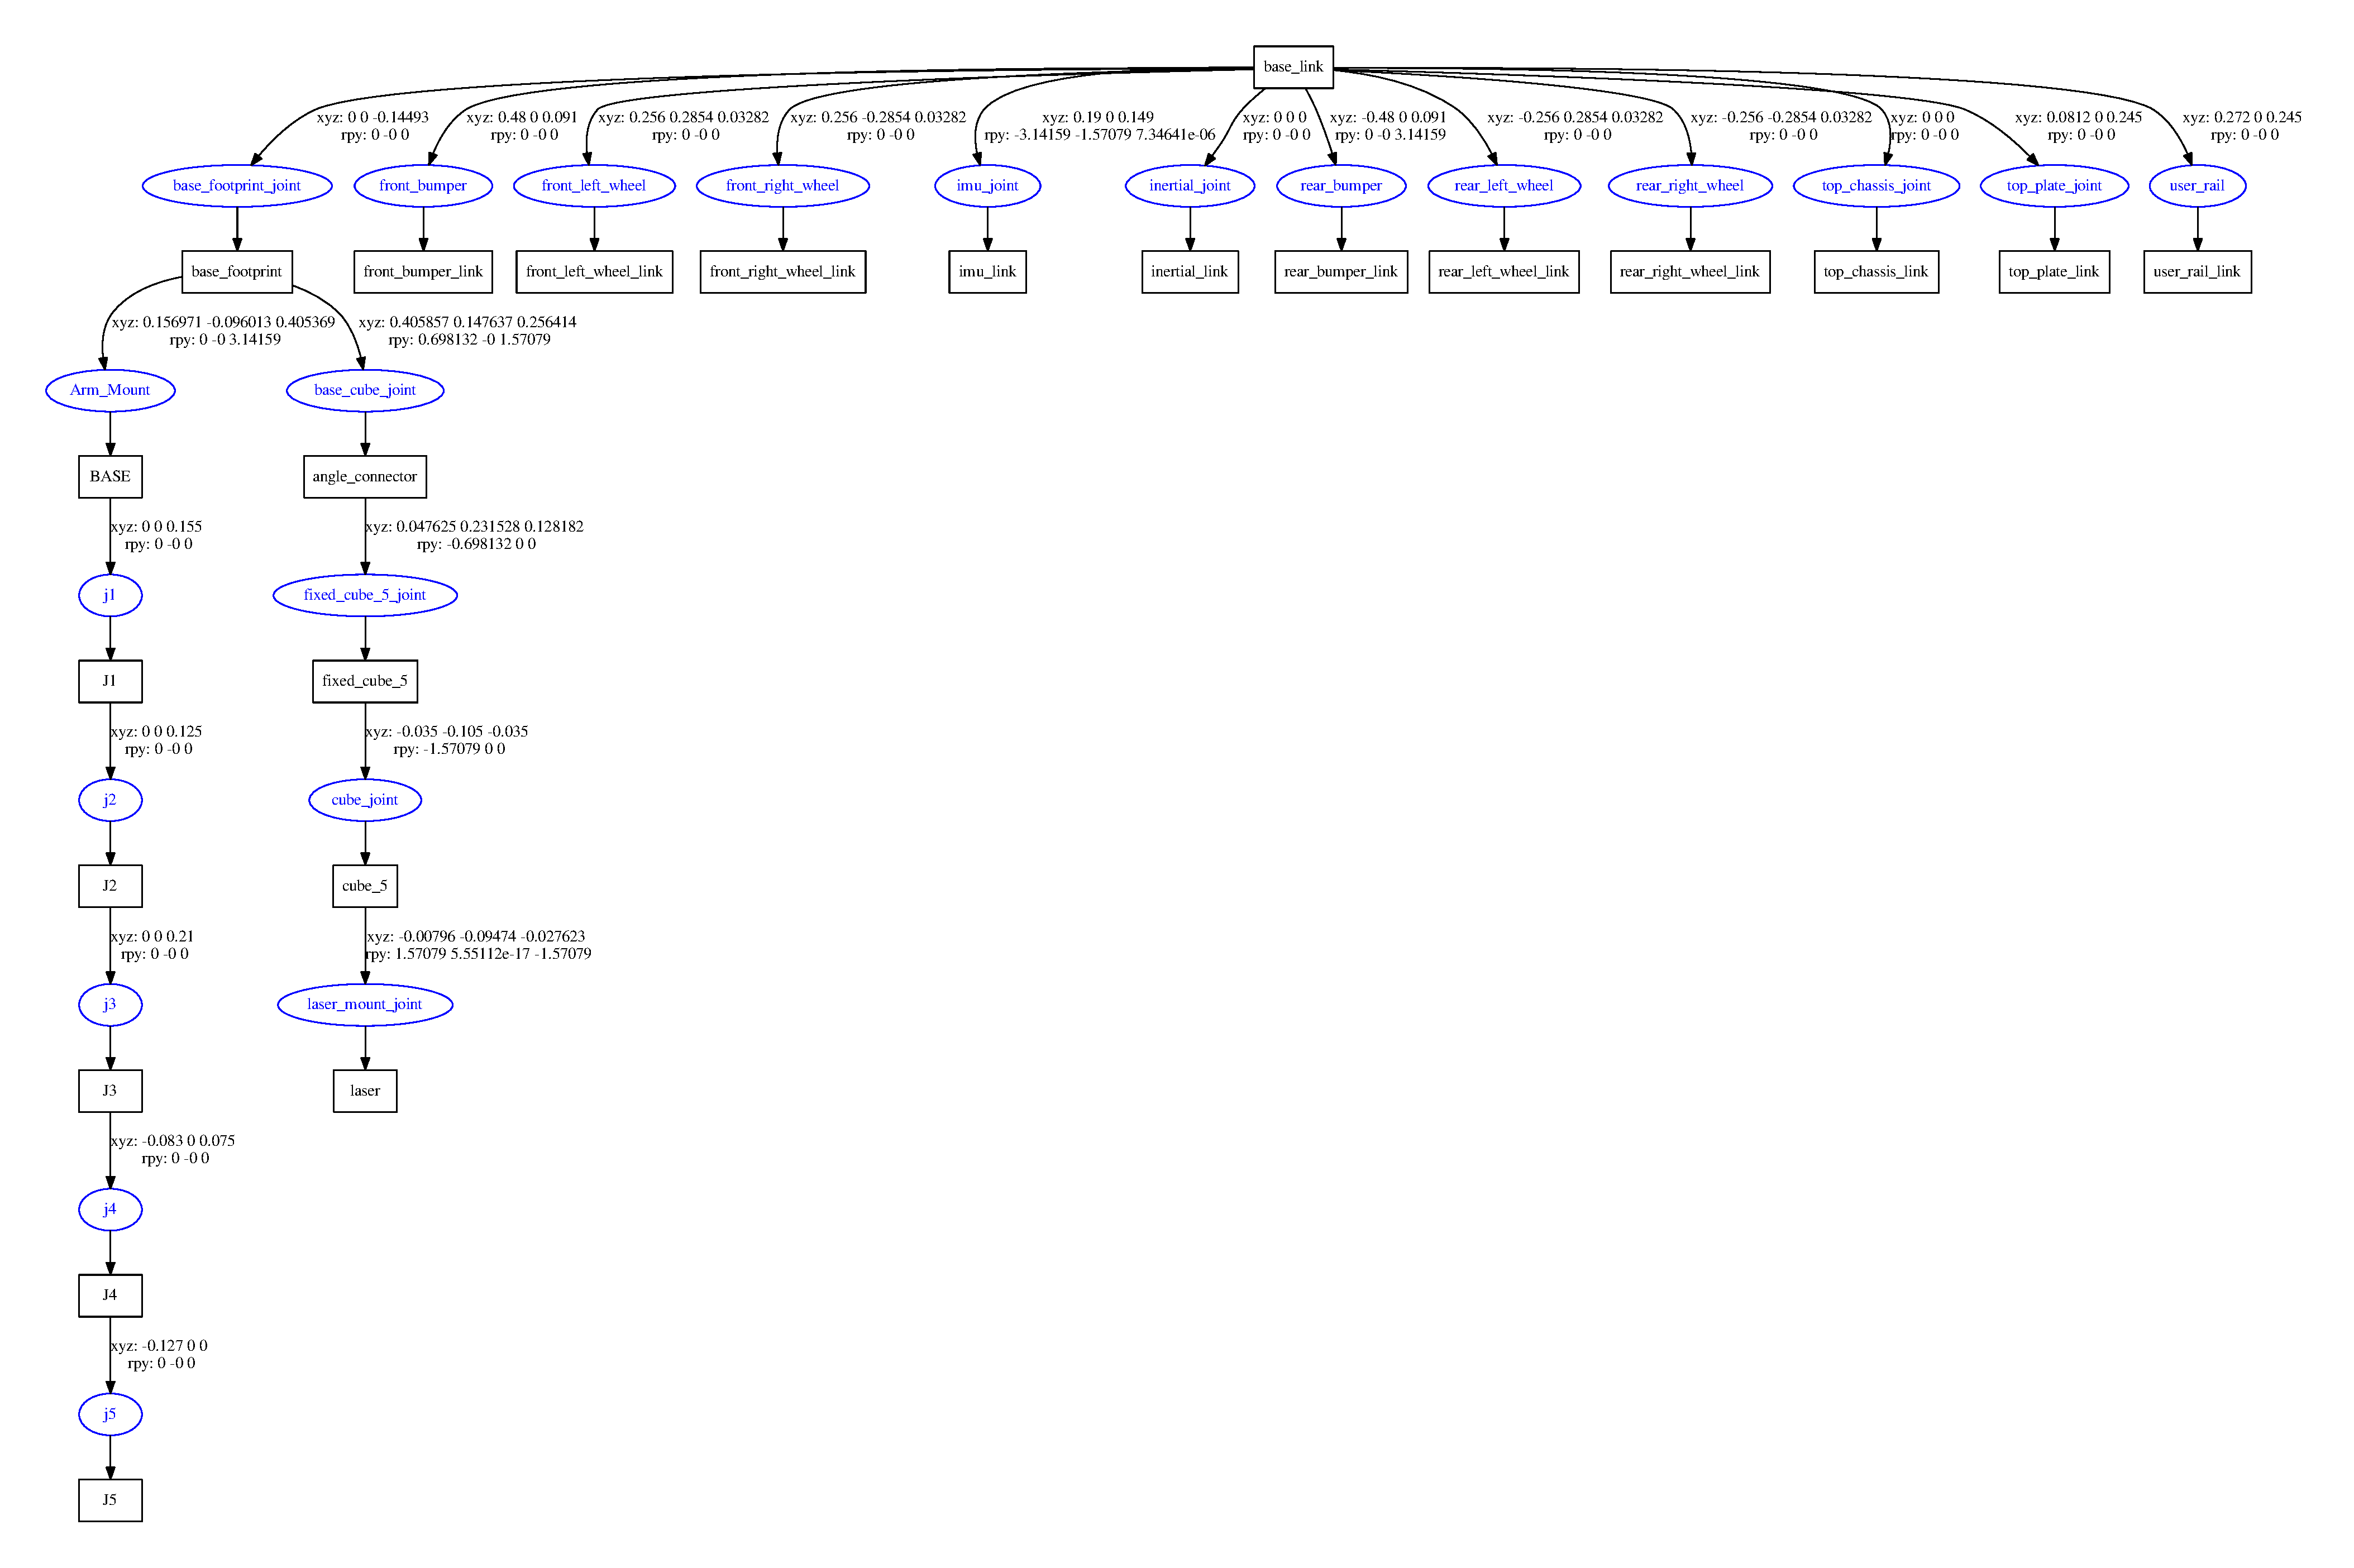
\includegraphics[width=0.8\textwidth]{Pics/husky.jpg}
    \caption{Husky UGV \cite{huskypage}}
    \label{fig:husky}
\end{figure}
\subsection{Husky Peripherals}

\begin{figure}[htb]
    \centering
    \includegraphics[width=\textwidth]{Pics/DSC0433.JPG}
    \caption{Husky with Peripherals Attached}
    \label{fig:peripherals}
\end{figure}
The Husky required a few modifications to support the additional hardware used. A top plate was machined to mount the manipulator as well as a mounting bracket for the nodding head servo. A trailer hitch was installed and a trailer was built to allow the Husky to tow additional batteries, a generator, and the controller for the manipulator.\\
\subsection{DENSO VP6242}
\begin{figure}[H]
    \centering
    \includegraphics[width=0.6\textwidth]{Pics/denso.png}
    \caption{DENSO VP6242 Manipulator \cite{densopage}}
    \label{fig:densofig}
\end{figure}
%https://www.denso-wave.com/en/robot/product/five-six/vp.html
The final product will likely use hydraulics to position the shotcreting and scanning end-effector. Since the payload and forces will require a high strength and rigidity manipulator, using electric motors would be infeasible. Designing a manipulator for this task is outside the scope of this research, so a suitable analogue was chosen. The requirements of the manipulator is that it can position its end-effector with 6 degrees-of-freedom like the final version, but does not require the same workspace, strength, or rigidity the final product would in order to accurately position the end-effector and apply shotcrete. The DENSO manipulator shown in Figure \ref{fig:densofig} was chosen since it fulfils all the application requirements and was available at \acrshort{uoit} for use in this work. It has a maximum reach of 432 mm and a maximum payload of 2.5 kg.\\ 
\subsection{LMS101}

\begin{figure}[H]
    \centering
    \includegraphics[width=0.25\textwidth]{Pics/sick.png}
    \caption{SICK LMS101 \acrshort{lidar} \cite{sickpage}}
    \label{fig:sick}
\end{figure}
%https://www.sick.com/de/en/detection-and-ranging-solutions/2d-\acrshort{lidar}-sensors/lms1xx/lms101-10000/p/p346868?ff_data=JmZmX2lkPXAzNDY4NjgmZmZfbWFzdGVySWQ9cDM0Njg2OCZmZl90aXRsZT1MTVMxMDEtMTAwMDAmZmZfcXVlcnk9JmZmX3Bvcz04JmZmX29yaWdQb3M9OCZmZl9wYWdlPTEmZmZfcGFnZVNpemU9OCZmZl9vcmlnUGFnZVNpemU9OCZmZl9zaW1pPTkzLjA=
The LMS101 shown in Figure \ref{fig:sick} is a \acrshort{lidar} scanner manufactured by SICK. It has an aperture angle of 270$\degree$, angular resolution of 0.25$\degree$ at 25 Hz, and optimal range of 0.5 m - 20 m. SICK is a well know brand of \acrshort{lidar} scanners, with lots of software drivers available for the various systems it works with. The \acrshort{ros} driver for this \acrshort{lidar} does not natively support 0.25$\degree$ resolution, so it has been modified accordingly for this work. It has a systematic error of $\pm$30 mm and statistical error of 12 mm, though through testing it was found the \acrshort{lidar} performs much better in the given test conditions. With an Ingress Protection (\acrshort{ip}) rating of \acrshort{ip}65, it is suitable for indoor use but can be replaced with another model from the same family with equal performance but higher \acrshort{ip} rating (up to \acrshort{ip}67).\\
\subsection{Schunk Powercube PR70}
\begin{figure}[H]
    \centering
    \includegraphics[width=0.27\textwidth]{Pics/powercube.png}
    \caption{Schunk Powercube PR70 \cite{schunkpage}}
    \label{fig:schunk}
\end{figure}
The \acrshort{lidar} used must be mounted on a nodding head to generate 3D point clouds. The Powercube PR70 made by Schunk was chosen for this task partly since it was already an asset of the \acrshort{uoit} \acrshort{mars} Lab and can be seen in Figure \ref{fig:schunk}. The module has higher accuracy and payload than the application requires, but since it was an unused asset it was chosen for this application for practicality reasons. It has a nominal torque of 15 Nm, repeat accuracy of 0.03$\degree$, maximum angular velocity of 240$\degree$/s, and maximum acceleration of 960$\degree$/s$^2$. The Powercube PR70 can be seen mounted on the MASS with the LMS101 \acrshort{lidar} attached in Figure \ref{fig:lidarmass}.\\
\begin{figure}[H]
    \centering
    \includegraphics[width=0.67\textwidth]{Pics/zoom.jpg}
    \caption{MASS Nodding Head Assembly}
    \label{fig:lidarmass}
\end{figure}
\section{Software}
\label{sec:software}
All software integrated and developed for this research is intended for use within the \acrshort{ros} framework. Since \acrshort{ros} is an open source community with many packages available for use in research, it offers a wide selection of resources useful to this work.\\

Many of the tasks required for operation of the MASS have already been developed by the \acrshort{ros} community. Hardware drivers, motion controllers, \acrshort{lidar} scan to point cloud assemblers, navigation, and mapping packages are already available through \acrshort{ros}. The following packages are necessary for the MASS to function.\\
\subsection{RViz}
\label{sec:RViz}

Complete documentation on RViz can be found at \url{http://wiki.ros.org/RViz}\\

RViz is a powerful visualization tool developed for use with \acrshort{ros}. There is a large quantity of information that can be generated using \acrshort{ros} that is not easily interpreted without the use of an interactive graphical user interface. RViz allows users to view, interact with, interpret, and modify the data handled within \acrshort{ros}. RViz is an invaluable tool in mobile robotics: it can display a model of the robot, a map the robot has generated of its environment, the path it intends to follow, and display sensor data the robot acquires. The user can interact with RViz and send commands to the robot such as: position goals, movement commands, status changes, or selecting parts of the sensor data to be used in other software algorithms.\\

RViz is designed to be adaptable for whatever the operator needs. Custom tools and plugins are easily developed to make RViz helpful in the context it is used. In this work, a custom tool was implemented for selecting sections of the mine surface to be scanned or shotcreted. A custom plugin called the control panel was created to provide a user-friendly interface to command and control all relevant aspects of the MASS.\\

RViz configurations can be saved to a file and loaded at launch when the robot control system is brought online. The configuration file for this work sets the RViz environment in a way that is practical for the operator, but includes options to reveal information useful for debugging and research. For example, under most circumstances the point cloud representation of the mine surface should be shown but individual laser scans hidden. If the operator wanted to see the instantaneous view of the robot's environment represented as a laser scan, the topic's checkbox simply needs to be checked. When generating trajectories the surface path, surface normals, and end-effector path are shown, however, the operator may only want some or none of the information displayed so they are all easily hidden or shown. This is all accomplished through the ``Displays'' panel of RViz. The configuration file subscribes RViz to all the relevant topics and automatically hides the topics containing information that does not need to be displayed.\\

\subsection{Husky}

Complete documentation of the Husky package can be found at \url{http://wiki.ros.org/Robots/Husky}\\

The Husky package is made by Clearpath Robotics to provide \acrshort{ros} functionality to their Husky Unmanned Ground Vehicle (UGV). The package consists of the following subpackages:

\begin{itemize}
    \item \node{husky_base}
    \item \node{husky_bringup}
    \item \node{husky_gazebo}
    \item \node{husky_viz}
    \item \node{husky_control}
    \item \node{husky_description}
    \item \node{husky_msgs}
    \item \node{husky_navigation}
\end{itemize}

\paragraph{husky\_base}

The \node{husky_base} package provides the low level communication between \acrshort{ros} and the robot. It contains all the necessary drivers to allow the robot to operate under \acrshort{ros} control.\\

\paragraph{husky\_bringup}

The \node{husky_bringup} package contains a number of scripts to that launch all the necessary packages (like \node{husky_base}) for the robot to function. Many applications for the Husky robot are intended to be turnkey, so the bringup package allows the designer to set what packages to launch when the robot boots up. Using the bringup package the robot can be configured to commence its control system as soon as it is powered on.\\

\paragraph{husky\_gazebo}

Gazebo is a simulation tool used in \acrshort{ros}. With a fully defined robot model, Gazebo can simulate the robot in a user defined environment. If an operator intends to test their algorithms on a Husky robot, but does not have access to a physical robot they can test their software on a simulated version of the Husky. Similarly, if the operator wants to test their robot in a scenario that may cause damage to the robot or in an environment they are unable to create, they can use Gazebo to test their algorithms in simulation.\\

\paragraph{husky\_viz}

RViz configurations can be saved and loaded by \acrshort{ros}. The \node{husky_viz} package contains various configurations for RViz that optimize its configuration for use with the Husky.\\

\paragraph{husky\_control}

The package \node{husky_control} turns motion goals into actual robot motion. The motion goals are published using \acrshort{ros} topics and the \node{husky_control} package subscribes to these topics and moves the robot accordingly. The motion goals can be provided directly from the operator using an input device such as a joystick or generated from autonomous navigation packages acting on a goal location provided by the operator. The source of the motion commands does not affect how the package functions, so it is able to receive motion commands from a wide variety of sources as long as the commands are formatted using the appropriate \acrshort{ros} message type.\\ 

\paragraph{husky\_description}

In order to visualize the robot in the RViz environment, the robot requires a description. The robot description contains all the relevant information about the robot parts, which way they can move, what material they are, and how to visually represent them. The description also contains the relevant physical characteristics to simulate the robot in Gazebo. The \node{husky_description} package uses the Unified Robot Description Format (\acrshort{urdf}) to describe the model for the Husky UGV.\\

\paragraph{husky\_msgs}

To communicate with other packages, or within the Husky packages, custom messages for the Husky robot are used. The \node{husky_msgs} package contains these custom messages. An example of the HuskyStatus message can be found in Appendix \ref{app:huskystatus}

%\includecode[pythonstyle]{Code/HuskyStatus.msg}{HuskyStatus.msg}

\paragraph{husky\_navigation}

The \node{husky_navigation} package provides configurations and examples for using varous navigation packages with the Husky. It contains all the relevant information a navigation package requires to successfuly apply the navigation algorithm on the Husky. Parameters such as the robot's footprint size, how far away to stay from obstacles, what sort of behaviours to exhibit when encountering obstacles, and what sensor information is available are contained within the configuration files. Navigation packages configure their global and local planners with the files contained in the \node{husky_navigation} package. The configuration file for producing costmaps for use in navigation is shown in Appendix \ref{app:huskyconfig} . The package contains launch files to use various navigation packages with the Husky robot as well as demos that will launch the required accompanying packages. Launch files for \acrshort{amcl}, GMapping, Frontier Exploration, and Move Base packages are included as well as an empty map for use when the robot is being simulated in Gazebo.\\ 
\clearpage
\subsection{Move Base}

Complete documentation of the Move Base package can be found at \url{http://wiki.ros.org/move_base}\\

\begin{figure}[H]
    \centering
    \includegraphics[width=\textwidth]{Pics/overview_tf.png}
    \caption{Overview of the Move Base Package \cite{rosmovebase}}
    \label{fig:movebaseoverview}
\end{figure}

The \node{move_base} package takes high level commands such as a location goal and performs the necessary actions to drive the robot to that location. A graphical overview of the package is shown in Figure \ref{fig:movebaseoverview}. It divides the task among two planners, the global planner and the local planner. The global planner is responsible for creating the overall plan for the robot path. It uses a global costmap generated by the map server, which holds the map generated by the \acrshort{slam} algorithm or loaded from file. The global costmap includes things like the inflation layer, which acts as a safety buffer by creating a region surrounding any obstacles within the map that the robot cannot enter. The local costmap is generated based on what the robot's sensors currently detect. If a person were to walk in front of the robot they would appear in the local costmap and the local planner would generate a path around the obstacle, attempting to return to the path generated by the global planner. If a person or object is placed close enough to the robot such that the robot is now within the inflation layer of the obstacle, it is considered stuck. Once stuck, the robot must execute recovery behaviours to become unstuck. Figure \ref{fig:recovery} shows what recovery behaviours \node{move_base} uses to free itself. First the robot deletes obstacles from the map that are further away than a user specified distance. If the robot is then free to move, it will continue its navigation. If the robot is still stuck, it will rotate on the spot to get an updated view of its surroundings. If it still cannot move it will clear the map of all obstacles that are not within the area it needs to rotate in place. If it is still stuck, it will rotate once more to scan its environment for obstacles. Once the second clearing rotation is complete, if it is still unable to move, it will abort its current goal and release a message notifying the system it was unable to reach its target location.\\

\begin{figure}[H]
    \centering
    \includegraphics[width=\textwidth]{Pics/recovery_behaviors.png}
    \caption{Move Base Recovery Behaviours \cite{rosmovebase}}
    \label{fig:recovery}
\end{figure}

\subsection{Laser Assembler}


Complete documentation of the Laser Assembler package can be found at \url{http://wiki.ros.org/laser_assembler}\\

The \node{laser_assembler} package converts the stream of laser scan data to a point cloud. When the MASS creates a point cloud representation of its surroundings, it tells the \node{laser_assembler} package when to start and stop recording the laser scans generated by the LMS101 \acrshort{lidar} scanner. The assembler will store all of the laser scans, along with the coordinate frame transformation from a fixed frame to the \acrshort{lidar} frame at that moment. When the point cloud scan is complete, \node{laser_assembler} is notified and produces a point cloud in the coordinate frame requested by the user. Discussed further in Section \ref{sec:locsourceerror}, the parameter \var{ignore_laser_skew} can be set so that each point in the laser scan is transformed using the current pose of the \acrshort{lidar} rather than transforming the whole scan at once. Accuracy can be improved if the position of the nodding head is updated more than once during the time it takes to perform a single point cloud scan.\\

\subsection{Hector SLAM}

Complete documentation of the Hector \acrshort{slam} package can be found at \url{http://wiki.ros.org/hector_slam}\\

The \node{hector_slam} package contains the \node{hector_mapping} package used by the MASS to perform \acrshort{slam}. The two main \acrshort{slam} packages available for use with \acrshort{ros} are GMapping and Hector \acrshort{slam}. GMapping is a more popular algorithm, but requires odometry from the robot. Hector \acrshort{slam} can perform \acrshort{slam} without the need for odometry. While the MASS does measure its odometry, it is intended for use on uneven rocky ground and odometry may not be reliable. For that reason, Hector \acrshort{slam} was chosen as the \acrshort{slam} algorithm for use on the MASS. However, thanks to the modularity that \acrshort{ros} offers, it is a simple task to utilize other \acrshort{slam} algorithms like GMapping on the MASS.\\

\subsection{RQT Reconfigure}

Complete documentation of the RQT Reconfigure package can be found at \url{http://wiki.ros.org/rqt_reconfigure}\\

If a node has been configured with parameters that can change at runtime, \node{rqt_reconfigure} can be used to modify them. When the user launches the Graphical User Interface (\acrshort{gui}), it will poll the \acrshort{ros} parameter server to determine which nodes have dynamically reconfigurable variables and what their values and acceptable ranges are. It then presents the user with a window that shows a list of nodes on the left. When a node is selected, the configurable parameters are shown on the right, most often in the form of a slider bar. An example \node{rqt_reconfigure} \acrshort{gui} window can be seen in Figure \ref{fig:dyngui2}.

\begin{figure}[h]
    \centering
    \includegraphics[width=\textwidth]{Pics/dyngui.png}
    \caption{\texttt{rqt\_reconfigure} \acrshort{gui}}
    \label{fig:dyngui2}
\end{figure}

\subsection{The MASS ROS Package}
\label{sub:software}

A thorough discussion of the source code is provided in Chapter \ref{chap:code}, however, an overview of the MASS would be incomplete without mentioning the \acrshort{ros} package that provides its functionality. The complete code can be found in Appendix \ref{app:code}.\\ 

\begin{figure}[H]
    \centering
    \includegraphics[width=\textwidth]{Pics/sixpt9.png}
    \caption{RViz User Interface}
    \label{fig:panel}
\end{figure}

The main interface between the user and the control system occurs within an RViz window. Along with the regular features of RViz, this software adds a panel and a tool to the RViz interface. The additional features can be seen in Figure \ref{fig:panel} labeled as Control Panel (right) and Selection Tool (top). The code for the control panel is split between two files. For the system's current purpose, it would be far less functional to have a standalone \acrshort{gui} and not use RViz for visualization. Therefore, \node{control_dashboard} was designed as a plugin for RViz. As future work on this project continues, the need for RViz visualization may diminish, so the node was designed to make converting it to run without RViz a trivial task. Eventually, when this system is implemented in a mine, no graphical interface at all will be required on the machine itself. For that reason, the core functionality of the system lies in the \node{control_panel} node. The \node{control_dashboard} node simply relays the actions from the user interface to the \node{control_panel} node.\\

The \node{control_panel} node is the heart of the control system. It is responsible for calling the localization, trajectory generation, and thickness estimation services, as well as communication with the DENSO arm, Powercube servo, and Husky UGV. Other MASS-specific requirements such as cropping regions from the robots perception that are occupied by the robot itself or  modifying trajectory points to fit within the DENSO arm's workspace are performed by the \node{control_panel} node. \\

The main contribution of this work to the \acrshort{ros} community are the localization, trajectory generation, and thickness estimation services. These three services are intended to be as portable as possible so they can be useful in any robotics project, regardless of the system configuration. Should other researchers have a need for the service they provide, one simply needs to install the package and they will be able to launch the desired service from the terminal or their own launch file. Unfortunately, due to this document's confidentiality, the source code will not be made available, so the functionality of the compiled binaries are provided as-is. Any of the parameters that can be modified by the user are still accessible, but the source code cannot be viewed or modified.\\

\subsubsection{MASS GUI}
\label{sub:gui}

\begin{figure}[ht!]
    \centering
    \includegraphics[width=.7\textwidth]{Pics/guidrawing.pdf}
    \caption{MASS \acrshort{gui} Panel}
    \label{fig:thegui}
\end{figure}
%%%%%%%%%%%%%%%%%%%%%%%%%%%%%%%%%%%%%%%%%%%%%%%%%%%5
%FIX THIS FIGURE"CALCULATE THICKNESS"
%%%%%%%%%%%%%%%%%%%%%%%%%%%%%%55555

The tabs of the MASS \acrshort{gui} control panel can be seen in Figure \ref{fig:thegui}. The main tab, called ``Operation'' is for use while the robot is operating. The red Stop button is a software activated emergency stop. The operation tab has a \acrshort{lidar} scan button that commands the robot to perform a \acrshort{lidar} scan using the nodding head and displays the resulting point cloud in the RViz window. The Set Home button is pressed when the robot is in a location the operator intends to define as the origin. The home position is then used as the coordinate frame into which all other point clouds are transformed into. The Generate Trajectory button generates a trajectory based on the current selection. Clicking Apply Shotcrete performs the motions for shotcrete application. If no area is selected, the default region (modified using \node{rqt_reconfigure}) is used and the system enters autonomous shotcrete mode. While in autonomous shotcrete mode the system will apply shotcrete and advance the robot until it is halted using the Stop button. Every time a point cloud is acquired, it is saved to disk. The textbox allows the user to declare where they would like the point clouds to be saved. The interface for recording localization markers is also present and its usage is discussed in Section \ref{sub:admin}. The load button can be used to load the indicated point cloud file from disk for display or analysis purposes.\\

Though the shotcrete thickness is automatically saved and displayed after applying shotcrete, the user may want to perform additional thickness calculations with RViz data or previously saved data. Selecting an area of a point cloud, clicking Set Initial Cloud, and repeating the steps for the final point cloud allows the operator to calculate the shotcrete thickness at a specified region by pressing Calculate Thickness. If they simply want to calculate thickness from two previously saved files, the file names and locations can be entered and the calculation is performed upon pressing Estimate Thickness. The resulting data can be saved to disk using the Save button.\\

The Denso Control tab allows the user to manually command the manipulator. The user can initialize the arm, shut it down, or clear the errors. When sending a pose, the user can specify a target location and Point-to-Point motion (PTP), Continuous Path motion (CP), or use the Tool coordinate frame (T). Alternatively, the user can specify specific joint angles to move to. The user can also set the speed of the manipulator, or use the text box to send a command formatted using DENSO's WINCAPSIII communication protocol. The current robot pose is displayed as well.\\
\begin{table}[h!] 
\begin{tabular}{|L{.12\textwidth}|L{0.6\textwidth}|m{0.28\textwidth}}
\cline{1-2}
\multicolumn{1}{|c|}{\textbf{Button}} & \multicolumn{1}{c|}{\textbf{Function}} &  \\ \cline{1-2}
Arm Step & Allows user to step through manipulator trajectory one via point at a time& \\ \cline{1-2}
Reset & Reset the counter when stepping through trajectory via points& \\ \cline{1-2}
Marker Only & Display markers for via points instead of moving the manipulator& \\ \cline{1-2}
Set Home & Set home location& \\ \cline{1-2}
Generate Poses & Calculate required positions the robot must move to to apply shotcrete over selected area& \multirow{15}{*}{\begin{minipage}{.3\textwidth}
      %  \vspace{1pt}
      \begin{center}
            \includegraphics[width=\linewidth]{Pics/ttab.png}
      \captionof{figure}{MASS \acrshort{gui} Testing Tab}
    \label{fig:ttab}
		\end{center}       
    \end{minipage}} \\ \cline{1-2}
Pose Step & Move to next location& \\ \cline{1-2}
Ctr & Counter for tracking current via point& \\ \cline{1-2}
Generate Trajectory & Generates a trajectory based on the current selection or default area, then saves to location entered in the ``Trajectory Save Location'' field& \\ \cline{1-2}
Execute Trajectory & Moves manipulator to simulate shotcrete application or radiation scan& \\ \cline{1-2}
Plot Path & Show the intended path the robot will travel to reach the desired location& \\ \cline{1-2}
Execute Path & Move robot to desired location& \\ \cline{1-2}
Show Nav Goal & Show robot's desired location& \\ \cline{1-2}
Estimate Thickness & Calculate thickness from previous two point cloud scans& \\ \cline{1-2}
Nav Mode & Move \acrshort{lidar} nodding head to a position for navigation (-1.57 radians, other positions can be commanded by changing the value of the text box)& \\ \cline{1-2}
Localize & Localize the robot& \\ \cline{1-2}
Auto Crop & Automatically crop an area behind the robot that the trailer is likely to occupy from the point cloud& \\ \cline{1-2}
Load Scan & Load a point cloud from file and treat it as if it was a newly acquired scan& \\ \cline{1-2}
Load Trajectory & Load a trajectory from file (at the location specified under ``Trajectory Save Location'')& \\ \cline{1-2}
Reset Map & Reset the \acrshort{slam} map& \\ \cline{1-2}
Scan & Perform a \acrshort{lidar} scan& \\ \cline{1-2}

\end{tabular}
\caption{Testing Functions}
\label{tab:testing}
\end{table}
        

If the debug version is launched, the testing tab shown in Figure \ref{fig:ttab} is available. The testing tab has many features useful for testing and developing new algorithms. Table \ref{tab:testing} explains each button's function.\\

\clearpage
\section{Operation Overview}
\label{sec:manual}
This section is intended to serve as an overview of how the MASS performs the following tasks:
\begin{myitemize}
\item Setting the Home Coordinate Frame
\begin{myitemize}
\item Navigating the Robot to Home Position
\item Performing a Localization Scan
\end{myitemize}
\item Recording the Fiducial Marker
\begin{myitemize}
\item Selecting Marker Keypoints
\item Training Additional Markers
\end{myitemize}
\item Shotcrete Application
\begin{myitemize}
\item Applying Shotcrete to a Selected Area
\item Autonomous Shotcrete Application
\end{myitemize}
\item Shotcrete Thickness Estimation
\begin{myitemize}
\item Automatic Thickness Estimation
\item Thickness Estimation From File
\item Loading a Point Cloud From Disk
\item Estimating Shotcrete Thickness Between Two Selected Areas
\end{myitemize}
\end{myitemize}
\newpage
\begin{tabularx}{\textwidth}{p{0.4\textwidth} p{0.6\textwidth} }
    \multicolumn{2}{c}{\parbox{\textwidth}{\subsection{Setting the Home Coordinate Frame}}}\\ \toprule
    \multicolumn{2}{l}{\textbf{Navigating the Robot to the Home Position}}\\ \midrule
     \multicolumn{2}{l}{
     \begin{minipage}{\textwidth} 	
\scriptsize
     \textbf{Manual Navigation} The MASS can be driven using a standard USB joystick connected to any computer on the same network that hes been configured and running \acrshort{ros}.
     \end{minipage}
     }\\
      
      \\
\begin{minipage}{.4\textwidth} 	
\scriptsize
\raggedright
        \textbf{Autonomous Navigation} The MASS can autonomously navigate to a goal specified using the 2D Nav Goal tool located at the top of the RViz window (see Figure \ref{fig:goal2}). The MASS performs \acrshort{slam} as it is navigating and is capable of avoiding obstacles and planning paths around them. To set a goal click the RViz window where the robot should to navigate to, and drag the cursor in the direction the robot should face. A green arrow is shown representing the final position and orientation the navigation system will attempt to achieve. Though not required, it is recommended the operator perform a non-homing scan (by clicking the Scan button) so RViz can display a rendering of the environment.
      \end{minipage}%
      &
        \begin{minipage}{.6\textwidth}
        \vspace{1pt}
      \begin{center}
            \includegraphics[width=\linewidth]{Pics/Manual/afar_goal.png}
      \captionsetup[figure]{font=scriptsize}
      \captionof{figure}{Setting a Navigation Goal}
      \label{fig:goal2}
		\end{center}
    \end{minipage}
\end{tabularx}

\begin{tabularx}{\textwidth}{m{0.3\textwidth} m{0.7\textwidth} }
    \multicolumn{2}{l}{\textbf{Performing a Homing Scan}}\\ \midrule
\begin{minipage}{.3\textwidth} 	
\scriptsize
\raggedright
       Click the Set Home button on the Control Panel (see Figure \ref{fig:xx1}). All future scans will be localized to this coordinate frame.
      \end{minipage}%
      &
        \begin{minipage}{.7\textwidth}
        \vspace{1pt}
      \begin{center}
            \includegraphics[width=.5\linewidth]{Pics/Manual/sethome.png}
      \captionsetup[figure]{font=scriptsize}
      \captionof{figure}{Control Panel, Operation Tab. Set Home Button Highlighted}
      \label{fig:xx1}
		\end{center}
    \end{minipage}
\end{tabularx}
\newpage
\begin{tabularx}{\textwidth}{p{0.3\textwidth} p{0.7\textwidth} }
    \multicolumn{2}{c}{\parbox{\textwidth}{\subsection{Recording the Fiducial Marker}}}\\ \toprule
    \multicolumn{2}{l}{\textbf{Selecting Marker Keypoints}}\\ \midrule
\begin{minipage}{.3\textwidth} 	
\scriptsize
\raggedright
       Using the Selection Tool, click and drag to form a box surrounding the marker keypoint (see Figures \ref{fig:afar2} and \ref{fig:xx2}).
      \end{minipage}%
      &
        \begin{minipage}{.7\textwidth}
        \vspace{1pt}
      \begin{center}
            \includegraphics[width=\linewidth]{Pics/Manual/marker1_selecting.png}
      \captionsetup[figure]{font=scriptsize}
      \captionof{figure}{Selecting a Marker Keypoint}
      \label{fig:afar2}
		\end{center}
    \end{minipage}\\
    \multicolumn{2}{c}{\begin{minipage}{\textwidth}
        \vspace{1pt}
      \begin{center}
            \includegraphics[width=\linewidth]{Pics/Manual/marker_2view.png}
      \captionsetup[figure]{font=scriptsize}
      \captionof{figure}{Marker Keypoints are Easily Visible When Colours are Set to Indicate Intensity}
      \label{fig:xx2}
		\end{center}
    \end{minipage}}
\end{tabularx}

\begin{tabularx}{\textwidth}{m{0.3\textwidth} m{0.7\textwidth} }
 \multicolumn{2}{l}{\textbf{Selecting Marker Keypoints (Continued)}}\\ \midrule
 \begin{minipage}{.3\textwidth} 	
\scriptsize
\raggedright
       The selected points are highlighted in blue (see Figures \ref{fig:xx3} and \ref{fig:xx4}). Points with intensity below \var{intensity_min} (which can be changed using \node{rqt_reconfigure}) are automatically removed.
      \end{minipage}%
      &
        \begin{minipage}{.7\textwidth}
        \vspace{1pt}
      \begin{center}
            \includegraphics[width=\linewidth]{Pics/Manual/marker1_selected.png}
      \captionsetup[figure]{font=scriptsize}
      \captionof{figure}{Selected Points Highlighted in Blue}
      \label{fig:xx3}
		\end{center}
        \vspace{1pt}
      \begin{center}
            \includegraphics[width=\linewidth]{Pics/Manual/marker1_selected_zoom.png}
      \captionsetup[figure]{font=scriptsize}
      \captionof{figure}{A Closer View of the Selected Points}
      \label{fig:xx4}
		\end{center}
    \end{minipage}%
\end{tabularx}
\begin{tabularx}{\textwidth}{m{0.3\textwidth} m{0.7\textwidth} }
 \multicolumn{2}{l}{\textbf{Selecting Marker Keypoints (Continued)}}\\ \midrule
 \begin{minipage}{.3\textwidth} 	
\scriptsize
\raggedright
      Click the Cluster Pt. 1 button (see Figure \ref{fig:xx5}).
      \end{minipage}%
      &
        \begin{minipage}{.7\textwidth}
        \vspace{1pt}
      \begin{center}
            \includegraphics[width=.5\linewidth]{Pics/Manual/cluster1.png}
      \captionsetup[figure]{font=scriptsize}
      \captionof{figure}{Teaching the First Marker Keypoint}
      \label{fig:xx5}
		\end{center}
    \end{minipage}\\
     \begin{minipage}{.3\textwidth} 	
\scriptsize
\raggedright
      Repeat the process for the second and third marker keypoints (see Figures \ref{fig:xx7} and \ref{fig:xx8}).
      \end{minipage}%
      &
        \begin{minipage}{.7\textwidth}
        \vspace{1pt}
      \begin{center}
            \includegraphics[width=.5\linewidth]{Pics/Manual/cluster2.png}
      \captionsetup[figure]{font=scriptsize}
      \captionof{figure}{Teaching the Second Marker Keypoint}
      \label{fig:xx7}
		\end{center}
        \vspace{1pt}
      \begin{center}
            \includegraphics[width=.5\linewidth]{Pics/Manual/cluster3.png}
      \captionsetup[figure]{font=scriptsize}
      \captionof{figure}{Teaching the Third Marker Keypoint}
      \label{fig:xx8}
		\end{center}
    \end{minipage}%
\end{tabularx}
\begin{tabularx}{\textwidth}{m{0.3\textwidth} m{0.7\textwidth} }
 \multicolumn{2}{l}{\textbf{Selecting Marker Keypoints (Continued)}}\\ \midrule
         \begin{minipage}{.3\textwidth} 	
\scriptsize
\raggedright
      Once Complete, the text displays ``Marker Recorded''. The Auto Localize feature is automatically enabled, as indicated by the checkbox (see Figure \ref{fig:xx9}).
      \end{minipage}%
      &
        \begin{minipage}{.7\textwidth}
        \vspace{1pt}
      \begin{center}
            \includegraphics[width=.5\linewidth]{Pics/Manual/operation_recorded.png}
      \captionsetup[figure]{font=scriptsize}
      \captionof{figure}{Fiducial Marker Completed}
      \label{fig:xx9}
		\end{center}
    \end{minipage}
\end{tabularx}
\begin{tabularx}{\textwidth}{p{0.5\textwidth} p{0.5\textwidth} }
    \multicolumn{2}{l}{\textbf{Training Additional Markers}}\\ \midrule
\begin{minipage}{.5\textwidth} 	
\scriptsize
\raggedright
       Multiple fiducial markers can be used, the localization algorithm will select the best one to use for localization. All fiducial markers are stored in a file at the same location where point clouds are automatically saved. The point cloud and fiducial marker save location is indicated by the ``Point cloud Save Location'' text box in the operation tab of the Control Panel (see Figure \ref{fig:xx11}). Additional markers can be added using the same procedure as the first marker. New markers must be added using a localized point cloud if the operator requires all point clouds to be localized to the same coordinate frame. To localize a point cloud and teach a new marker, the robot must take a scan from a position that includes both the old marker keypoints as well as the new ones to be taught. Figure \ref{fig:afar2} shows a point cloud scan taken from a location in which two individual fiducial markers can be taught.
      \end{minipage}%
      &
        \begin{minipage}{.5\textwidth}
        \vspace{1pt}
      \begin{center}
            \includegraphics[width=.8\linewidth]{Pics/Manual/operation_save.png}
      \captionsetup[figure]{font=scriptsize}
      \captionof{figure}{Point Cloud Save Location is the Same as the Marker Save Location}
      \label{fig:xx11}
		\end{center}
    \end{minipage}
\end{tabularx}

\begin{tabularx}{\textwidth}{p{0.3\textwidth} p{0.7\textwidth} }
    \multicolumn{2}{c}{\parbox{\textwidth}{\subsection{Shotcrete Application}}}\\ \toprule
    \multicolumn{2}{l}{\textbf{Applying Shotcrete to a Selected Area}}\\ \midrule
\begin{minipage}{.3\textwidth} 	
\scriptsize
\raggedright
       To autonomously apply shotcrete to a selected area, use the Selection Tool located at the top of the RViz window and drag a box to encompass the desired area to apply shotcrete (see Figure \ref{fig:xx12}). More complex selections can be achieved by holding the keyboard's Ctrl button while selecting additional areas or points.
      \end{minipage}%
      &
        \begin{minipage}{.7\textwidth}
        \vspace{1pt}
      \begin{center}
            \includegraphics[width=\linewidth]{Pics/Manual/shotcrete_selecting.png}
      \captionsetup[figure]{font=scriptsize}
      \captionof{figure}{Manual Selection of Shotcrete Area}
      \label{fig:xx12}
		\end{center}
    \end{minipage}\\
		\begin{minipage}{.3\textwidth} 	
\scriptsize
\raggedright
       Once the desired area has been selected, press the Generate Trajectory button to generate a trajectory for the manipulator to follow (see Figures \ref{fig:xx13} and \ref{fig:xx14}).\\
       \vspace{2pt}
       \includegraphics[width=\linewidth]{Pics/Manual/operation_gen.png}
      \captionsetup[figure]{font=scriptsize}
      \captionof{figure}{Generate Trajectory Button}
    \label{fig:xx13}
      \end{minipage}%
      &
        \begin{minipage}{.7\textwidth}
        \vspace{1pt}
      \begin{center}
            \includegraphics[width=\linewidth]{Pics/Manual/shotcrete_trajectory.png}
      \captionsetup[figure]{font=scriptsize}
      \captionof{figure}{Trajectory Generated from Shotcrete Selection}
      \label{fig:xx14}
		\end{center}
    \end{minipage}
\end{tabularx}

\begin{tabularx}{\textwidth}{p{0.3\textwidth} p{0.7\textwidth} }
    \multicolumn{2}{l}{\textbf{Applying Shotcrete to a Selected Area (Continued)}}\\ \midrule
\begin{minipage}{.3\textwidth} 	
\scriptsize
\raggedright
       Inspect the trajectory to ensure a satisfactory result. Via points outside the robot's workspace are shown in red, while via points within the workspace are shown in green (see Figure \ref{fig:xx15}). The path along the surface the robot will follow is shown in red, the path the end-effector will follow is shown in green, and the surface normals are shown in blue.
      \end{minipage}%
      &
        \begin{minipage}{.7\textwidth}
        \vspace{1pt}
      \begin{center}
            \includegraphics[width=\linewidth]{Pics/Manual/goodbadpts_robot.png}
      \captionsetup[figure]{font=scriptsize}
      \captionof{figure}{Robot Workspace (White) with Via Points Highlighted in Red (Outside Workspace) or Green (Within Workspace)}
      \label{fig:xx15}
		\end{center}
    \end{minipage}\\
		\begin{minipage}{.3\textwidth} 	
\scriptsize
\raggedright
       If the trajectory is satisfactory the operator can press the Apply Shotcrete button (see Figure \ref{fig:xx16}). Once pressed, the robot will navigate to the wall if necessary and the via points outside the manipulator's workspace are moved. As the algorithm executes the trajectory, the blue lines connecting the surface path to the via points are turned white after each via point is completed.
      \end{minipage}%
      &
        \begin{minipage}{.7\textwidth}
        \vspace{1pt}
      \begin{center}
            \includegraphics[width=.5\linewidth]{Pics/Manual/operation_apply.png}
      \captionsetup[figure]{font=scriptsize}
      \captionof{figure}{Apply Shotcrete Button}
      \label{fig:xx16}
		\end{center}
    \end{minipage}
\end{tabularx}
%
\newpage
\begin{tabularx}{\textwidth}{p{\textwidth}}
    \textbf{Autonomous Shotcrete Application}\\ \midrule
\begin{minipage}{.7\textwidth} 	
\scriptsize
\raggedright
       When the robot autonomously applies shotcrete it acts similar to a wall following robot; it will follow the mine surface beside it until the operator commands it to stop using the STOP button on the Control Panel (see Figures \ref{fig:xx10} and \ref{fig:xx17}).
\end{minipage}%
\begin{minipage}{.3\textwidth}
        \vspace{1pt}
      \begin{center}
            \includegraphics[width=.8\linewidth]{Pics/Manual/operation_stop.png}
      \captionsetup[figure]{font=scriptsize}
      \captionof{figure}{STOP Button}
      \label{fig:xx10}
		\end{center}
		\end{minipage}
      \begin{center}
            \includegraphics[width=\linewidth]{Pics/Manual/3pose_frame.png}
            \captionsetup[figure]{font=scriptsize}
      \captionof{figure}{Multiple Trajectories Generated as Robot Autonomously Follows Mine Applying Shotcrete}
      \label{fig:xx17}
		\end{center}
    \begin{minipage}{.3\textwidth} 	
\scriptsize
\raggedright
       The operator should navigate the robot to a location where the automatic shotcreting can begin, using the Set Goal tool as shown in Figure \ref{fig:goal2}. Once there, the operator should ensure the automatic shotcrete selection area, as well as the automatic occlusion area is suitable. The area of the mine scan that is kept for trajectory generation is shown in blue and can be changed using the \node{rqt_reconfigure} panel (see Figure \ref{fig:xx18}).
      \end{minipage}%
        \begin{minipage}{.7\textwidth}
        \vspace{1pt}
      \begin{center}
            \includegraphics[width=\linewidth]{Pics/Manual/autokeep.png}
      \captionsetup[figure]{font=scriptsize}
      \captionof{figure}{Points to be Kept for Automatic Shotcrete Application}
      \label{fig:xx18}
		\end{center}
    \end{minipage}
\end{tabularx}

\begin{tabularx}{\textwidth}{p{0.3\textwidth} p{0.7\textwidth} }
    \multicolumn{2}{l}{\textbf{Autonomous Shotcrete Application (Continued)}}\\ \midrule
    \begin{minipage}{.3\textwidth} 	
\scriptsize
\raggedright
     To ensure the robot does not attempt to apply shotcrete to itself it is important to ensure the occlusion zone is set appropriately. Using \node{rqt_reconfigure}, the area to be cropped in which the robot's components may be detected by the \acrshort{lidar} scan is set. The volume enclosed by orange lines will be automatically removed before shotcrete trajectory generation (see Figure \ref{fig:xx19}).
      \end{minipage}%
      &
        \begin{minipage}{.7\textwidth}
        \vspace{1pt}
      \begin{center}
            \includegraphics[width=\linewidth]{Pics/Manual/auto_occlude.png}
            \captionsetup[figure]{justification=raggedright}
      \captionsetup[figure]{font=scriptsize}
      \captionof{figure}{Points to be Removed Before Trajectory Generation}
      \label{fig:xx19}
		\end{center}
    \end{minipage}\\
    \begin{minipage}{.3\textwidth} 	
\scriptsize
\raggedright
       If no area of the mine has been selected for manual shotcrete application, the operator can click the Apply Shotcrete button to begin the automatic shotcrete application (see Figure \ref{fig:xx20}).
      \end{minipage}%
      &
        \begin{minipage}{.7\textwidth}
        \vspace{1pt}
      \begin{center}
            \includegraphics[width=.5\linewidth]{Pics/Manual/operation_apply.png}
      \captionsetup[figure]{font=scriptsize}
      \captionof{figure}{Clicking Apply Shotcrete Without a Selection Begins the Autonomous Shotcreting Process}
      \label{fig:xx20}
		\end{center}
    \end{minipage}
\end{tabularx}


\begin{tabularx}{\textwidth}{p{0.3\textwidth} p{0.7\textwidth} }
    \multicolumn{2}{c}{\parbox{\textwidth}{\subsection{Shotcrete Thickness Estimation}}}\\ \toprule
    \multicolumn{2}{l}{\textbf{Automatic Thickness Estimation}}\\ \midrule
\begin{minipage}{.3\textwidth} 	
\scriptsize
\raggedright
       During normal operation, the shotcrete thickness is automatically estimated after shotcrete has been applied (see Figure \ref{fig:thickeg2}).
      \end{minipage}%
      &
        \begin{minipage}{.7\textwidth}
        \vspace{1pt}
      \begin{center}
            \includegraphics[width=\linewidth]{Pics/Manual/thickness_result.png}
      \captionsetup[figure]{font=scriptsize}
      \captionof{figure}{Automatic Thickness Estimate}\label{fig:thickeg2}
		\end{center}
    \end{minipage}
\end{tabularx}

\begin{tabularx}{\textwidth}{p{0.5\textwidth} p{0.5\textwidth} }
    \multicolumn{2}{l}{\textbf{Thickness Estimation From File}}\\ \midrule
\begin{minipage}{.5\textwidth} 	
\scriptsize
\raggedright
       To apply the shotcrete thickness estimation algorithm to point clouds saved to disk, use the Thickness tab of the Control Panel to indicate the file location of the initial and final scans, then click the Estimate Thickness button (see Figure \ref{fig:xx22}). The resulting estimate can be saved by clicking the save button.
      \end{minipage}%
      &
        \begin{minipage}{.5\textwidth}
        \vspace{1pt}
      \begin{center}
            \includegraphics[width=.7\linewidth]{Pics/Manual/thickness_estimate.png}
            \captionsetup[figure]{font=scriptsize,justification=raggedright}
      \captionof{figure}{Estimating Shotcrete Thickness From two Saved Scans}
      \label{fig:xx22}
		\end{center}
    \end{minipage}\\
    \multicolumn{2}{l}{\textbf{Loading a Point Cloud From Disk}}\\ \midrule
    \begin{minipage}{.5\textwidth} 	
\scriptsize
\raggedright
       To load a point cloud, scan, or thickness estimate from disk, click the Load button on the Operation tab of the Control Panel (see Figure \ref{fig:load2}).
      \end{minipage}%
      &
        \begin{minipage}{.5\textwidth}
        \vspace{1pt}
      \begin{center}
            \includegraphics[width=.7\linewidth]{Pics/Manual/operation_load.png}
      \captionsetup[figure]{font=scriptsize}
      \captionof{figure}{Point Cloud Files can be Loaded From Disk}
      \label{fig:load2}
		\end{center}
    \end{minipage}
\end{tabularx}

\begin{tabularx}{\textwidth}{p{0.3\textwidth} p{0.7\textwidth} }
    \multicolumn{2}{l}{\textbf{Estimating Shotcrete Thickness Between Two Selected Areas}}\\ \midrule
\begin{minipage}{.3\textwidth} 	
\scriptsize
\raggedright
       To estimate shotcrete thickness for a specific area, the first point cloud should be loaded from disk (see Figure \ref{fig:load2}). Using the Selection Tool, select an area slightly larger than the desired measurement area and click Set Initial Cloud (see Figures \ref{fig:xx24} and \ref{fig:xx25}). Load the final point cloud, and select the area in which to estimate thickness (see Figure \ref{fig:xx26}). Click the Set Final Cloud button. Once the initial and final point clouds have been set the user can click Calculate Thickness to generate a thickness estimate like the one shown in Figure \ref{fig:thickeg2}.
      \end{minipage}%
      &
        \begin{minipage}{.7\textwidth}
        \vspace{1pt}
      \begin{center}
            \includegraphics[width=.5\linewidth]{Pics/Manual/thickness_selection.png}
      \captionsetup[figure]{font=scriptsize}
      \captionof{figure}{Calculating Shotcrete Thickness for a Specific Selection}
      \label{fig:xx24}
		\end{center}
    \end{minipage}\\
        \vspace{1pt}\\
    \multicolumn{2}{c}{
    \begin{minipage}{.5\textwidth}
        \vspace{1pt}
      \begin{center}
            \includegraphics[width=\linewidth]{Pics/Manual/pre_selecting.png}
      \begin{minipage}{.8\linewidth}
      \captionsetup[figure]{font=scriptsize}
      \captionof{figure}{Selecting the Initial Point Cloud}
      \label{fig:xx25}
      \end{minipage}
		\end{center}
    \end{minipage}%
    \begin{minipage}{.5\textwidth}
        \vspace{1pt}
      \begin{center}
            \includegraphics[width=\linewidth]{Pics/Manual/post_selecting.png}
      \begin{minipage}{.8\linewidth}
      \captionsetup[figure]{font=scriptsize}
      \captionof{figure}{Selecting the Final Point Cloud}
      \label{fig:xx26}
      \end{minipage}
		\end{center}
    \end{minipage}
    }
\end{tabularx}\\
\clearpage
\section{Chapter Summary}

The hardware and software components of the MASS were discussed. The Husky UGV, DENSO manipulator, SICK \acrshort{lidar}, are Powercube servo are the main hardware systems used. The software packages for RViz, Husky, and \acrshort{slam} along with their dependent packages are available through \acrshort{ros} and were configured to operate with the MASS. A brief overview of the MASS software package was presented, and a pseudo manual describing the typical operation of the MASS features was provided.\\

%  \chapter{Software}
\label{chap:code}
\section{Chapter Summary}
This chapter discusses the complete ROS package built and presents the algorithms used in the MASS source code. Much of the code simply facilitates the handling and communication of data across the various nodes as well as inputting and parsing commands from the user. Since the system was primarily designed to be a research platform many of the testing, debugging, and experimentation portions of the code have been included in the final version for future work. The ROS package contains typical elements such as \node{CMakeLists.txt}, \node{package.xml}, messages, services, configuration and launch files, URDF descriptions, source code, and headers. The following sections discuss the package framework and core functionality using pseudo code algorithms. The complete code can be found in Appendix \ref{app:code}. Beginning with a discussion of the ROS framework this chapter presents the novel algorithms developed for this work.\\
\section{Package Files}

A package is the most atomic structure in ROS, meaning it is the root of all projects created for ROS. At its minimum, a package is simply a directory containing \node{package.xml}. As the package grows to contain its own software nodes, a \node{CMakeLists.txt} file is used to define which software files need to be compiled. Other components of a ROS package can include messages, services, dependencies, header files, and source code. Packages big and small are all self contained so they can be easily shared and implemented on other systems.\\

\subsection{package.xml}
The file \node{package.xml} contains the package name, version number, description, maintainer, and license. As well, it contains a list of all the other packages necessary to build and run the package. It contains a reference to \node{plugin_description.xml} so the compiler is aware there are custom plugins for this package and what file they are located in.\\

The \node{package.xml} for the MASS can be found in Appendix \ref{app:pack}.
\subsection{plugin\_description.xml}
This package uses a custom plugin and tool for RViz. The plugin, called ``Control Panel'' is a ``ControlPanel'' object in the ``control\_panel'' namespace and extends the ``RViz::Panel'' class. The ``Selection Tool'' tool is a fork of the ``SelectionTool'' class called ``selection\_tool'' and extends the ``RViz::Tool'' class. It has been modified to function more effectively when used with the MASS GUI.\\

The \node{plugin_description.xml} for the MASS can be found in Appendix \ref{app:plug}.
\subsection{CMakeLists.txt}
The \node{CMakeLists.txt} file is the first file ROS uses when compiling the package. Within this file all the nodes, messages, services, configuration files, and dependencies are declared. They can be found listed in Table \ref{tab:cmakelists}. The file can be found in Appendix \ref{app:cmake}.\\
\begin{table}[h!]
\begin{adjustwidth}{-.5in}{-.5in}  
\begin{tabular}{|c|c|c|c|}
\hline
Nodes & Messages & Services & Configuration Files \\ \hline
\parbox[t]{4cm}{
\tabitem cube\_node \\
\tabitem denso\_node \\
\tabitem joint\_fusion\_node \\
\tabitem cloud\_localizer \\
\tabitem thickness\_server \\
\tabitem trajectory\_server \\} & \parbox[t]{4cm}{
\tabitem cube\_msg \\
\tabitem arm\_msg \\
\tabitem trajectory\_point \\
\tabitem trajectory\_msg \\
\tabitem trajectory\_array \\
\tabitem empty \\} & \parbox[t]{4cm}{
\tabitem localize\_cloud \\
\tabitem thickness\_service \\
\tabitem trajectory\_service \\} & \parbox[t]{4cm}{
\tabitem param\_config \\
\tabitem localize\_config \\
\tabitem trajectory\_config \\}\\ \hline
\end{tabular}
\caption[]{Contents of the \node{CMakeLists.txt} file}
\label{tab:cmakelists}
\end{adjustwidth}
\end{table}
\section{Launch Files}
Two launch files are provided: \node{main.launch} and \node{simulation.launch}. The launch files appear in their entirety in Appendix \ref{app:launch} and are explained as follows: 

\subsection{main.launch}

The \node{main.launch} file performs the following actions (using the syntax \node{package_name} : \node{node_name}):
\begin{itemize}

\item Include other launch files

\begin{itemize}

\item \node{MASS_husky_description} : \node{description.launch}
\item \node{husky_control} : \node{control.launch}
\item \node{husky_control} : \node{teleop.launch}

\end{itemize}

\item Launch nodes
\begin{itemize}

\item \node{MASS} : \node{cube_node}
\item \node{MASS} : \node{denso_node}
\item \node{MASS} : \node{joint_fusion}
\item \node{um6} : \node{um6_driver}
\item \node{move_base} : \node{move_base}
\item \node{lms1xx} : \node{LMS1xx_node}
\item \node{laser_filters} : \node{scan_to_scan_filter_chain}
\item \node{laser_assembler} : \node{laser_scan_assembler}
\item \node{hector_mapping} : \node{hector_mapping}
\item \node{RViz} : \node{RViz}
\item \node{rqt_reconfigure} : \node{rqt_reconfigure}
\item \node{tf} : \node{static_transform_publisher}

\end{itemize}

\item Launch services

\begin{itemize}

\item \node{MASS} : \node{cloud_localizer}
\item \node{MASS} : \node{trajectory_server}
\item \node{MASS} : \node{thickness_server}

\end{itemize}

\item Load configuration files

\begin{itemize}

\item \node{MASS} : \node{RViz_main.RViz}
\item \node{MASS} : \node{my_laser_config.yaml}
\item \node{husky_navigation} : \node{planner.yaml}
\item \node{husky_navigation} : \node{costmap_common.yaml}
\item \node{husky_navigation} : \node{costmap_local.yaml}
\item \node{husky_navigation} : \node{costmap_global_laser.yaml}
\end{itemize}

\end{itemize}

Since the MASS is a modified Husky UGV, the URDF description has been modified accordingly. A separate package for the modified URDF description called \node{MASS_husky_description} was made and the launch file containing the URDF description is included. Including a launch file within another launch file effectively copies all the code from the included launch file into the main launch file, but keeping them separate allows the user to keep the package modular and makes the launch file more compact and readable.\\

Following the inclusion of the URDF launch file, the Husky specific nodes are launched. The node responsible for communication between ROS and the Husky is called \node{husky_node}. When launched the parameters indicating which USB port it is connected to, the controller and diagnostic frequencies, wheel diameter, and speed and acceleration limits are set. Launch files from the \node{husky_control} package are included to instruct the controller how to properly handle \node{move_base} velocity and joystick commands, perform EKF localization, and display the Husky's movements in RViz. As well, the driver for the IMU on board the Husky is launched.\\

When the \node{move_base} node is launched the local and global planner configurations are loaded from a file or stated explicitly. Parameters like the Husky footprint size and recovery behaviours are not intended to be modified frequently, so they are stored in a file. The user may want to change other parameters like maximum velocity and the safety buffer from obstacles, or have multiple launch files with different settings. They are able to set or overwrite parameters from a configuration file explicitly in the launch file. Whether the parameters are set using a configuration file or from the launch file the effect is the same, however, the launch file takes priority so if the same parameter is set using both methods, the values in the launch file will be used.\\

When the \node{scan_to_scan_filter} node is launched it loads the configuration file that sets the LiDAR distance, intensity, and angular range to be used. As well, the LiDAR driver and \node{laser_scan_assembler} node is launched.\\

To publish the joint states of the robot, \node{cube_node}, \node{denso_node}, and \node{joint_fusion} are launched. The \node{joint_fusion} node combines the individual joint states from the other two nodes and publishes them as a single joint state message. The node \node{robot_state_publisher} uses the joint state message and the URDF file to publish the tf tree of the robot. The tf tree, as its name implies, is a tree structure of coordinate frame transformations. It is used by ROS to calculate the transformation between any two frames present and is used by RViz along with the URDF to display the current pose of the MASS and its manipulator.\\

The node \node{hector_mapping} performs SLAM while the robot is operating. When launched, the parameter for \var{base_frame} is set so it has a point of reference for its local coordinate frame.\\

When RViz is launched, ``RViz\_MASS.RViz'' is loaded to configure the RViz environment optimally for use with the MASS. Different `.RViz' files can be loaded for different scenarios, for example the ``RViz\_debug.RViz'' configuration is loaded when debugging because it displays many of the point clouds and visualizations that are helpful in debugging but unnecessary during normal operation.\\

The final section of the launch file launches the trajectory generation, localization, and thickness estimation services, the \node{rqt_reconfigure} GUI, and a \node{static_transform_publisher} that aligns the map to the world coordinate frame.\\

\subsection{simulation.launch}

For demonstration, experimentation, or debugging purposes, the user may want to launch an environment where they can use the MASS control panel in RViz with the localization, trajectory generation, and thickness estimation services without connecting to the physical robot. The \node{simulation.launch} file allows the user to do so by launching the following nodes and files:

\begin{itemize}

\item \node{MASS_husky_description} : \node{description.launch}
\item \node{MASS} : \node{joint_fusion}
\item \node{MASS} : \node{cloud_localizer}
\item \node{MASS} : \node{trajectory_server}
\item \node{MASS} : \node{thickness_server}
\item \node{RViz} : \node{RViz}
\item \node{MASS} : \node{RViz_debug.RViz}
\item \node{rqt_reconfigure} : \node{rqt_reconfigure}
\item \node{tf} : \node{static_transform_publisher}
\end{itemize}

\section{Messages}

Messages are a convenient way of grouping together variables into a single object. In this work, messages are used to send commands from \node{control_panel} to \node{denso_node} and \node{cube_node}. As well, custom messages were generated for use in determining the fiducial marker location and transmitting arm trajectories between nodes.\\

\subsection{trajectory\_point.msg}
\includecode{CleanedCode/msg/trajectory_point.msg}{trajectory\_point.msg}
Each point in the trajectory requires the position and surface normal at that position. The \var{trajectory_point} message contains that information as well as a \var{d} parameter. The \var{d} parameter is used when sorting lines of points to keep track of the approximate total distance along the surface (see Section \ref{sec:sortlines}).\\
\subsection{trajectory\_msg.msg}
\label{sec:trajmsg}
\includecode{CleanedCode/msg/trajectory_msg.msg}{trajectory\_msg.msg}
Messages in ROS can contain a limited variety of datatypes, but among them is the ability to include other messages or arrays of messages (see \url{http://wiki.ros.org/msg}). For the manipulator trajectories in this work, an array of \var{trajectory_point} messages is used.\\

\subsection{arm\_msg.msg}
\includecode{CleanedCode/msg/arm_msg.msg}{arm\_msg.msg}
The \var{arm_msg} message was designed to make it easy to send commands to the DENSO manipulator. The message contains 32-bit floats that can hold joint positions, XYZ positions (and the rotation around each axis), velocity, and acceleration. The \var{fig} integer allows the user to command the desired shoulder, elbow, and wrist configuration (\var{fig} table can be found in Appendix \ref{sec:fig}). The \var{pose} boolean is used to tell \node{denso_node} whether the XYZ values are positions or velocities. Since the DENSO manipulator can perform continuous path motion as well as point-to-point, the \var{motion_type} variable holds the desired motion behaviour. For testing and debugging purposes it may become necessary to manually generate a command string to send to the DENSO controller, so the string \var{user_string} was added to incorporate that functionality.\\

\subsection{cube\_msg.msg}
\includecode{CleanedCode/msg/cube_msg.msg}{cube\_msg.msg}
Originally the \node{cube_node} was designed to handle multiple Powercubes at once, but as research continued, the Powercube manipulator was replaced with the DENSO manipulator. Additional joint variables can easily be added should a user want to control multiple Powercubes, however, control of a single Powercube is all that is required within this work. The variables in the \var{cube_msg} message contain the desired position or velocity (depending on the value of \var{pose}), the maximum velocity (used only in position commands), and maximum acceleration allowed to reach the position (or velocity) goal.\\

\subsection{marker\_val.msg}
\includecode{CleanedCode/msg/marker_val.msg}{marker\_val.msg}
When the localization algorithm attempts to detect the markers, it is possible there may be many potential keypoints to choose from, meaning multiple marker candidates exist. The \var{marker_val} message is used to hold them so a sorting algorithm can find the closest match in the marker file. The i, j, and k variables hold the position of the first, second, and third keypoint within the array of keypoint candidates. The \var{val} variable holds a value representing how accurately the keypoints match the recorded keypoints in the marker file. The value for \var{val} is calculated using a weighted sum of the the distances between $P_1-P_2$, $P_2-P_3$, and the angle between $\mathbf{P_1P_2}$ and $\mathbf{P_2P_3}$. \\

\section{Services}
In ROS services are able to receive and return variables and messages. In order for ROS to determine what messages or variables to expect and what to return, a `.srv' file is used to explicitly declare the messages a service is expecting and what message it will return. The division between incoming and outgoing data is marked by a line containing ``\texttt{----}''. The three services built for this work are the ``Cloud Localization Service'', ``Trajectory Generation Service'', and ``Thickness Estimation Service'' discussed below, their source code can be found in Appendix \ref{app:sourcesrv}.\\
\subsection{Cloud Localization Service}
\includecode{CleanedCode/srv/localize_cloud.srv}{localize\_cloud.srv}
This localization service expects a point cloud to localize, a string to indicate the location of the marker file, and a boolean used to instruct the service if the point cloud scan is to set the world coordinate frame or localize within it. The service returns the localized cloud and a transformation matrix from the robot's frame of reference to the marker's frame.\\
%
%\lstinputlisting[
%style=C++style,
%caption={[pointcloud\_localization\_service.cpp (lines 86, 91, and 100)] pointcloud\_localization\_service.cpp (lines 86, 91, and 100)},
%linerange={86-86,91-91,100-100},]{CleanedCode/src/pointcloud_localization_service.cpp}
  
Three helper functions were used to simplify the main portions of the code. They perform dot products, cross products, and normalized cross products. The main function initializes the node, advertises its service on the \node{\localize_pcd} topic, and configures a visualization to show the possible marker keypoint locations on topic \node{\visualization_marker}. The \node{rqt_reconfigure} callbacks are set and the visualization marker style is set. The node then ``spins'', meaning it will wait until a message is received and execute the appropriate callback. A callback function ROS was written for each topic the service subscribes to.\\

The callback function to localize the cloud is explained in Algorithm \ref{alg:localize}.
\begin{algorithm}[H]
\caption{Localization Algorithm}
\label{alg:localize}
\begin{algorithmic}[1]
\begin{raggedright}
\Function{localize}{Input cloud, Marker filename, Homing boolean}
\State Filter incoming point cloud based on user-defined maximum and minimum intensity values
\If {User requests homing scan}
\State Change input point cloud coordinate frame from \node{base_footprint} to \node{world}
\Else
\State Open marker.bag file to retrieve markers
\State Cluster point cloud points to generate list of keypoint candidates
\State Determine which keypoint candidates correspond to marker keypoints
\State Select best marker (based on correspondence)
\State Transform input point cloud to world coordinate frame \EndIf
\EndFunction\\
\Return Localized point cloud
\end{raggedright}
\end{algorithmic}
\end{algorithm}

\subsubsection{Clustering Points}
Since the LiDAR scanner's resolution is smaller than the size of the marker keypoint, it will typically detect multiple data points per marker keypoint. The keypoint candidates are determined by taking the mean location of all data points within a certain radius and with sufficiently high reflected intensity. The algorithm to cluster data points into keypoint candidates is Algorithm \ref{alg:cluster} (note, the data has already been filtered for intensity so all data points remaining are possible marker keypoints).

\begin{algorithm}[H]
\caption{Clustering Algorithm}
\label{alg:cluster}
\begin{algorithmic}[1]
\algnotext{EndFor}
\begin{raggedright}
\Function{cluster}{Intensity filtered input cloud}
\ForAll{Points in input cloud}
\If{Intensity $>0$}
\State Add point to clustering array
\ForAll{Remaining points in input cloud}
\If{Distance between points is less than CLUSTER\_DISTANCE \textbf{AND} Intensity $>0$}\\
\Comment{CLUSTER\_DISTANCE set by user using rqt\_reconfigure}
\State Add point to clustering array
\State Set point intensity to 0 (so it doesn't get added to another cluster)
\EndIf
\EndFor
\State Average all points in clustering array
\State Add averaged point to array of keypoint candidates
\State Clear clustering array
\EndIf
\EndFor
\EndFunction\\
\Return Array of keypoint candidates
\end{raggedright}
\end{algorithmic}
\end{algorithm}
\subsubsection{Determining Marker Keypoints}
After the clustering algorithm, an array of keypoint candidates is produced. If there are less than three points, the marker has not been detected and the service reports a failure. If there are three or more keypoint candidates, they must be checked to ensure they fit the marker model. If there are multiple groups of keypoint candidates that fit the marker model, the best fit is chosen. If none of the keypoints fit the marker model, the service reports it could not detect the marker. Once the marker is located, a $3\times3$ matrix holding the XYZ positions of the marker keypoints and a $4\times4$ transformation matrix of its position relative to the scanner is stored in the matrices indicated by the pointers passed to the function. The algorithm for fitting keypoint candidates and selecting the best three is Algorithm \ref{alg:keypoint}.
\begin{spacing}{0.8}
\begin{algorithm}[H]
\caption{Keypoint Selection Algorithm}
\label{alg:keypoint}
\begin{algorithmic}[1]
\algnotext{EndFor}
\begin{raggedright}
\Function{locate\_marker}{Array of keypoint candidates, Marker file location, Pointer to return transformation martix}
\State Clear marker\_found boolean
\For{$ i:=1 $ \textbf{to} Size of candidate array}
\For{$ j:=1 $ \textbf{to} Size of candidate array}
\For{$ k:=1 $ \textbf{to} Size of candidate array}
\If{$i\neq j\neq k$}
\State Calculate distances between $i$, $j$, and $k$
\State Calculate dot product between vector $\mathbf{ji}$ and $\mathbf{jk}$
\For{Each marker in the marker file}
\State Calculate accuracy by comparing distances and dot product to marker file
\EndFor
\State Store $i$, $j$, $k$, accuracy, and marker index in array of marker candidates
\If{Marker candidate is within user defined accuracy limits}
\State Set marker candidate as valid
\If{Valid marker candidate already exists}
\State Set optimization flag
\EndIf
\EndIf
\EndIf
\EndFor
\EndFor
\EndFor
\If{One or more marker candidates are found}
\State Set marker\_found boolean
\If{Optimization flag is set}
\State Select most accurate candidate
\EndIf
\State Calculate and return transformation matrix using the indicated pointer \
\EndIf
\EndFunction\\
\Return Boolean indicating if marker was located
\end{raggedright}
\end{algorithmic}
\end{algorithm}
\end{spacing}
The code for calculating the transformation matrix (where P1, P2, and P3 correspond to $i$, $j$, and $k$ from algorithm \ref{alg:keypoint}) can be found in Appendix \ref{app:tmat}.\\

\subsection{Trajectory Generation  Service}
\includecode{CleanedCode/srv/trajectory_service.srv}{trajectory\_service.srv}
The trajectory generation service expects two point clouds and returns a \var{trajectory_msg} formatted trajectory (see Section \ref{sec:trajmsg}). The first point cloud, called \var{cloud_in}, is the area to generate a trajectory for. The second point cloud, \var{cloud_surface}, is the entire scan. The full surface scan is required for calculating surface normals at the edge of the selected area, since without it only a portion of the surrounding data points would be used to calculate the surface normal.\\

When the service launches it advertises itself on the \node{/trajectory_gen} topic. It then configures the publishers responsible for displaying the markers that show the end-effector path, surface path, surface normals, via points within the workspace, and via points outside the workspace. Finally it configures the callback for \node{rqt_reconfigure}. Once initialized, the service waits to be called upon.\\

When the service is called, it executes the \func{generate} function. The trajectory is generated in two stages, the first is for vertical sections and the second is for horizontal (overhead) sections as per Algorithms \ref{alg:trajv} and \ref{alg:trajh}.
\begin{algorithm}[H]
\caption{Trajectory Generation Algorithm (Vertical Sections)}
\label{alg:trajv}
\begin{algorithmic}[1]
\algnotext{EndFor}
\begin{raggedright}
\Function{generate}{Point cloud selection, Full point cloud}
\State Extract intersection between horizontal plane (at \var{mid_height}) and point cloud selection
\State Sort extracted line (at \var{chunk_radius} downsampling)
\For{$ ctr:=1 $ \textbf{to} Size of sorted line}
\State Extract intersection between vertical plane (passing through robot centre and point of sorted line at index \var{ctr}) and point cloud selection
\State Sort extracted line (at \var{downsample_radius} downsampling)
\State Add extracted line to \var{rib_array}
\EndFor
\State Set \var{height} = 0
\While{\var{height} < (\var{wall_height} \textbf{and} max height of point cloud selection)}
\For{$ ctr:=1 $ \textbf{to} Size of \var{rib_array}}
\State Select point at \var{height} in rib at index \var{ctr} of \var{rib_array}
\State Calculate point normal (using full point cloud), apply offset, and add point to \var{arm_trajectory}
\EndFor
\State Increment \var{height} by \var{height_step}
\For{$ ctr:=$ Size of \var{rib_array} \textbf{to} $1$}
\State Select point at \var{height} in rib \var{ctr} of \var{rib_array}
\State Calculate point normal, apply offset, and add point to \var{arm_trajectory}
\EndFor
\If{\var{height} > (\var{wall_height} \textbf{or} max height of point cloud selection)}
\State Break while loop
\EndIf
\State Increment \var{height} by \var{height_step}
\EndWhile
\EndFunction\\
\Return Arm Trajectory
\end{raggedright}
\end{algorithmic}
\end{algorithm}
\begin{spacing}{0.8}
\begin{algorithm}[H]
\caption{Trajectory Generation Algorithm (Horizontal Sections)}
\label{alg:trajh}
\begin{algorithmic}[1]
\algnotext{EndFor}
\begin{raggedright}
\Function{generate}{Point cloud selection, Full point cloud}
\State Extract intersection between vertical plane (through robot's X-axis) and point cloud selection
\If{No intersection exists}
\State Extract intersection between vertical plane (through robot's Y-axis) and point cloud selection
\EndIf
\If{No intersection exists}
\State Extract intersection between vertical plane (parallel with robot's X-axis, but intersecting nearest point in point cloud selection
\EndIf 
\State Sort extracted line (at \var{chunk_radius} downsampling)
\For{$ ctr:=1 $ \textbf{to} Size of sorted line}
\State Rotate a horizontal plane around robot's Y-axis (or X-axis) to intersect with point \var{ctr} of sorted line
\State Extract intersection between rotated plane and point cloud selection
\State Sort extracted line (at \var{downsample_radius} downsampling)
\State Add extracted line to \var{rib_array}
\EndFor
\State \var{height} = \var{wall_height}
\While{\var{height} < max height of point cloud selection (measured along the surface)}
\For{$ ctr:=1 $ \textbf{to} Size of \var{rib_array}}
\State Select point at \var{height} in rib \var{ctr} of \var{rib_array}
\State Calculate point normal, apply offset, and add point to \var{arm_trajectory}
\EndFor
\State Increment \var{height} by \var{height_step}
\For{$ ctr:=$ Size of \var{rib_array} \textbf{to} $1$}
\State Select point at \var{height} in rib \var{ctr} of \var{rib_array}
\State Calculate point normal, apply offset, and add point to \var{arm_trajectory}
\EndFor
\If{\var{height} > max height of point cloud selection (measured along the surface)}
\State Break while loop
\EndIf
\State Increment \var{height} by \var{height_step}
\EndWhile
\EndFunction\\
\Return Arm Trajectory
\end{raggedright}
\end{algorithmic}
\end{algorithm}
\end{spacing}
\subsection{Thickness Estimation Service}

The thickness estimation service is fairly simple and straightforward. For each point in the source cloud the nearest neighbour is found in the target cloud. The intensity value of that data point is replaced with the value of the distance to the nearest neighbour. The service automatically saves the calculated point cloud to a file. For the most accurate results, it is best to choose the point cloud with the highest point density as the target cloud.\\

The algorithm for calculating shotcrete thickness is Algorithm \ref{alg:thick}.

\begin{algorithm}[H]
\caption{Thickness Estimation Algorithm}
\label{alg:thick}
\begin{algorithmic}[1]
\algnotext{EndFor}
\begin{raggedright}
\Function{calculate}{Source point cloud, Target point cloud}
\ForAll{Points in source}
\State Find nearest point in target
\State Calculate distance between points
\State Replace point's intensity value with absolute distance measured
\EndFor
\State Save point cloud to disk
\EndFunction\\
\Return Point cloud with thickness values
\end{raggedright}
\end{algorithmic}
\end{algorithm}

\subsection{Map Reset Service}
The Hector SLAM package does not have the functionality to halt the mapping process. It also does not support 3D mapping so it will not take in to account the rotation of the LiDAR's nodding head. This means that when the nodding head moves to generate a point cloud, the SLAM algorithm will attempt to interpret the new laser scan data as robot motion, most often ending up distorting the map and losing its position. For this reason, the map must be reset after every point cloud scan. The Hector SLAM package can reset the map upon receiving an empty service call on the \node{move_base/clear_costmaps} topic, so the message ``empty.srv'' was generated to perform such actions. Before each reset the map is saved to disk so SLAM can resume after the scan is taken.\\

\section{Configuration Files}
Configuration files used by the \node{rqt_reconfigure} node make the parameters within them available for modification through the \node{rqt_reconfigure} GUI. A configuration file contains the variables' name, data type, priority level, and text description as well as the default, maximum, and minimum value. The configuration files for this work can be found in Appendix \ref{app:cfgs}.\\

The control panel configuration file (ROS File \ref{code:cpcfg} in Appendix \ref{app:cfgs}) generates an interface in the \node{rqt_reconfigure} GUI which can be seen in Figure \ref{fig:cpgui}. The variable names are seen on the left of the slider bars, with the maximum and minimum values on the right and left side of the slider respectively. To the right of the slider bars, the user can manually enter in a number instead of using the slider. When the user hovers the mouse over a variable, the text description appears in a black box (as shown for the ``init\_clear'' parameter in Figure \ref{fig:cpgui}).

\begin{figure}[h]
    \centering
    \includegraphics[width=\textwidth]{Pics/control_panel.png}
    \caption{\texttt{rqt\_reconfigure} GUI for Control Panel Parameters}
    \label{fig:cpgui}
\end{figure}

\subsection{YAML Files}
Files with the `.yaml' extension are used for parameters that should be easily changed, but do not require modification during runtime. For example, the data from the laser scanner is filtered before being used to create point clouds. Due to the range of motion of the nodding head and the angular bounds of the laser scanner, it is capable of detecting portions of the robot to which it is mounted. This data can be cropped out at a later time, but it is more efficient to limit the distance, angle, and intensity values of the LiDAR data so that the \node{laser_scan_assembler} node does not have to handle as much data. The ROS File \ref{code:yaml} in Appendix \ref{app:cfgs} shows the `.yaml' configuration file for the \node{scan_filter_chain} node that sets the minimum distance, maximum angle, and maximum intensity values to keep.\\

\section{URDF}
The Unified Robot Description Format (URDF) is an XML format for representing a robot model. A URDF file representing the system in this work can be found in Appendix \ref{app:urdf}. The Graphviz diagram for visualizing the URDF model can be seen in Figure \ref{fig:urdf}. In the URDF file each link within the robot is given a name. The links are shown in Figure \ref{fig:urdf} as black boxes. The links are then connected with joints (either revolute or prismatic), shown as blue ellipses in Figure \ref{fig:urdf}. The position and orientation of each link is specified in the URDF, as well as the 3D mesh for visualizing the links. With a complete URDF, ROS only requires the angle (or extension) of each joint in order to display a 3D rendered model of the robot within RViz. The \node{robot_state_publisher} node listens for the joint angles and broadcasts the tf tree containing the coordinate frame transformations for each link.\\

\begin{figure}[h]
    \centering
    \includegraphics[width=\textwidth]{Pics/urdf.png}
    \caption{Graphviz Diagram of URDF File}
    \label{fig:urdf}
\end{figure}

\section{Header Files}
Header files are often used to define various global functions and variables to be made available to the corresponding source files that include it. These globals can be made public or private, restricting or allowing them to be accessed by other programs. The two source files requiring custom headers are \node{control_panel.cpp} and \node{control_dashboard.cpp}. As well, the \node{marker_selector} plugin has a custom header file for its internal functionality. The header files can be found in Appendix \ref{app:headers}.\\

\section{Source Files}
The main component of the source code for this work is the control panel. The \node{control_dashboard} is embedded as a panel in RViz and creates the QNode object \node{control_panel}. The reason for this configuration is modularity; if the control panel is to be moved out of the RViz environment, \node{control_panel} is left unchanged and \node{control_dashboard} is replaced with a standalone container for the GUI. The complete code for all source files can be found in Appendix \ref{app:source}.
\subsection{Control Dashboard}
The \node{control_dashboard} node was designed as an RViz panel with the intention to make it replaceable should the designer decide to develop a standalone application instead of using RViz as the environment for the GUI. To mimimize the amount of work required to convert the panel to a standalone application, as little code as possible was implemented in the node.\\

The dashboard performs the actions that an operator would during manual control. When the robot is finished taking a scan, the dashboard instructs \node{control_panel} to generate a trajectory. Upon completion of the shotcrete application or radiation scan the dashboard instructs \node{control_panel} to advance the robot to complete its task if required. After arriving at its new location the dashboard instructs the robot to begin a scan and generate a trajectory. The GUI layout uses \node{control_dashboard} to call the appropriate \node{control_panel} functions when the GUI buttons are pressed, meaning all commands are passed through \node{control_dashboard}.\\
\subsection{Control Panel}
The \node{control_panel} node is the central controller of the system. It is responsible for executing the commands that are passed to it through \node{control_dashboard}. This node performs the following tasks:
\begin{itemize}
\item Visualization
\begin{itemize}
\item Default Shotcrete Region
\item Auto-crop Region
\item Move\_base Goal
\item Laser Scanned Point Clouds
\item Manipulator Workspace
\item Trajectory Display
\begin{itemize}
\item Surface Path
\item End-effector Path
\item Surface Normal
\item Via Points Within Manipulator Workspace
\item Via Points Outside Manipulator Workspace
\end{itemize}
\end{itemize}
\item Calling Services
\begin{itemize}
\item Laser Assembler
\item Localization
\item Trajectory Generation
\item Thickness Estimation
\item Map Reset
\end{itemize}
\item Publishing Motion Commands
\begin{itemize}
\item Powercube (Nodding Head)
\item DENSO (Manipulator)
\item Husky (Base)
\end{itemize}
\item Administrative Functions
\begin{itemize}
\item Set World Coordinate Frame
\item Save Point Cloud Selection
\item Load Trajectory From File
\item Step Through Via Points
\item Software Emergency Stop
\item Set Manipulator Speed
\item Manually Initiate Laser Scan
\item Record Marker Location
\item Load Point Cloud From File
\end{itemize}
\item Internally Used Functions
\begin{itemize}
\item Delete Point From Point Cloud
\item Find and Delete Nearest Neighbour
\item Delete Points Within Area
\item Calculate Vector Length
\item Calculate Dot Product
\item Calculate Manipulator Roll, Pitch, and Yaw for a Given Surface Normal
\item Move Via Point to Workspace
\item Find and Publish New Base Goal Location
\end{itemize}
\end{itemize}
\subsubsection{Visualization}
Figures \ref{fig:cropb} to \ref{fig:cands} show the visualizations that \node{control_panel} generates. The default area the robot will apply shotcrete to is shown in teal in Figure \ref{fig:cropb}. Since the scanner can capture some of the robot body when generating point clouds, it is useful to automatically crop a region that is likely to contain the robot but unlikely to contain sections of the mine surface. The auto-crop region is shown in orange in Figure \ref{fig:cropb}. For debugging purposes, the user may want to be aware of the keypoint candidates the localization algorithm is using, so they are published as translucent red boxes as seen in Figure \ref{fig:cands}. When a trajectory is generated many of the via points must be moved to within the manipulator's workspace due to its small size. The points that must be moved are shown as red points in Figure \ref{fig:trajviz} and the points that lie within the workspace are shown in green.\\
\begin{figure}[h]
    \centering
    \includegraphics[width=\textwidth]{Pics/cropboxespng.png}
    \caption{Auto-crop (Orange) and Auto-shotcrete (Teal) Area Visualizations}
    \label{fig:cropb}
\end{figure}
\begin{figure}[h]
    \centering
    \includegraphics[width=\textwidth]{Pics/workspace.png}
    \caption{Visualization of DENSO Workspace}
    \label{fig:worksp}
\end{figure}
\begin{figure}[h]
    \centering
    \includegraphics[width=\textwidth]{Pics/traj_viz.png}
    \caption{Trajectory Vizualization: Surface Path (Red), End-Effector Path (Green), Surface Normal (Blue), Via Points Within Manipulator Workspace (Green), and Via Points Outside Manipulator Workspace (Red)}
    \label{fig:trajviz}
\end{figure}
\begin{figure}[h]
    \centering
    \includegraphics[width=\textwidth]{Pics/candidates.png}
    \caption{Potential Keypoint Candidates Highlighted (Red)}
    \label{fig:cands}
\end{figure}
\subsubsection{Administrative Functions}
\label{sub:admin}
Most of the administrative functions are functions that are used internally during autonomous mode. When manually controlling the robot, they can be controlled directly. Through the use of administrative functions, the operator can manually drive the robot to a location of their choosing, perform a scan (and either set the location as the world coordinate frame or localize the cloud within it), generate a trajectory, load a trajectory or point cloud from file, step through the via points one at a time, set the manipulator speed, or initiate a software E-Stop (emergency stop) command. \\

The \node{control_panel} is also responsible for recording the marker location. The process of recording a marker is presented in Section \ref{sec:manual}. Internally, \node{control_panel} will calculate the marker parameters and store them in a file for use during localization.\\
\subsubsection{Internal Functions}
In order to perform the required tasks, several internally used functions were created. The ``Delete Point From Point Cloud'', ``Find and Delete Nearest Neighbour'', and ``Delete Points Within Area'' are used together to remove sections of a point cloud or line of points. These functions essentially downsample the point cloud but remove the downsampled points as they are used.\\

Since the manipulator workspace is small, it is difficult to test if the trajectory execution is successful. For this reason a function that moves via points outside the workspace to within the workspace is used. This function will move points too far for the manipulator to reach without losing degrees-of-freedom to the edge of the dextrous workspace. At that point, rather than using the surface normal, the end-effector aims in the direction defined by the vector from the workspace centre to the new via point location. As well, there is a wedge shaped region directly behind the manipulator base which it cannot reach, so points located within that region are moved inside the workspace as well. These actions are performed with the help of the vector length function.\\

The manipulator requires Roll-Pitch-Yaw (RPY) angles to define the end-effector orientation, so \node{control_panel} calculates the corresponding RPY at each via point based on the surface normal. To calculate the RPY, a dot product function is used. While there are dot product functions available through the Eigen software library, they require different data types, so a modified dot product function was used instead of performing data type conversions on the input and output values of the Eigen dot product function.\\

Once the MASS has completed scanning or shotcreting the area within its workspace, it may be required to advance the base to a new location to complete the scanning or shotcreting process. It does so using Algorithm \ref{alg:findandmove}.

\begin{algorithm}[H]
\caption{Base Advance Algorithm}
\label{alg:findandmove}
\begin{algorithmic}[1]
\State Acquire point cloud of surroundings
\State Extract a horizontal line from the point cloud at \var{mid_height}
\State Crop any points that are within the area that was already scanned or shotcreted
\State Crop an area the size of the workspace, centred at the nearest remaining point
\State Determine surface normal at nearest remaining point, using original point cloud for normal calculation
\State Define \node{move_base} goal using desired offset from wall
\State Define \node{move_base} orientation using cross product between Z-axis and surface normal
\State Publish \node{move_base} goal and visualization marker
\end{algorithmic}
\end{algorithm}

\subsection{DENSO and Powercube Nodes}
The \node{denso_node} is the software interface between the DENSO controller and the ROS package. The node communicates with the DENSO controller via ethernet using the bCAP communication protocol and WINCAPSIII formatted messages. Once a connection has been established the node activates the remote operation task loaded on the controller and begins sending commands. After initialization, the node waits for an \var{arm_msg} message and sends the appropriate commands to the controller to achieve the desired manipulator motion. When not sending commands to the manipulator, it is reading the manipulator's current pose so it can broadcast the data for other nodes to receive such as the \node{robot_state_publisher} responsible for displaying the 3D model of the robot in RViz\\

The \node{cube_node} sends commands to the Powercube through a virtual serial port created by the USB-Serial adapter connected to the system. Similar to the DENSO node, it initializes the device and waits for \var{cube_msg} messages to instruct it to move the Powercube to the desired position. Like the DENSO node, it also continually broadcasts the position of the Powercube.\\
 
\subsection{Additional Nodes}
To follow the data flow structure of this package a modified version of RViz's Selection Tool was used. The modifications allow the tool to broadcast a point cloud message containing the selected points. This point cloud message is used by the various services and nodes that require user input (such as marker selection or area to shotcrete).\\

The \node{robot_state_publisher} node that provides the tf tree of the system was designed to have a single source broadcasting the joint states over the \node{/joint_states} topic. However, in this work there are three separate sources for joint states: the Husky, the DENSO manipulator, and the Powercube module. To fuse the three separate joint state messages the \node{joint_state_fusion} node subscribes to all three sources and broadcasts a single message containing the pose of all the links in the system.\\
\section{External Packages and Libraries}
\label{sec:extpkg}
Some of the nodes in this work use messages or functions created for other packages. In order for the nodes to use them, they must be added as a dependency to the package. The dependencies in this work are:

\begin{itemize}
\item roscpp
\item rospy
\item RViz
\item sensor\_msgs
\item std\_msgs
\item tf
\item urdf 
\item diagnostic\_updater
\item schunk\_libm5api
\item diagnostic\_msgs
\item control\_msgs
\item message\_generation
\item message\_filters
\item actionlib\_msgs
\item laser\_assembler
\item pcl\_conversions 
\item pcl\_ros 
\item MASS\_husky\_description
\item qt\_build
\item dynamic\_reconfigure
\end{itemize}
%  \chapter{Testing and Results}
\label{chap:testing}

\section{Mock Mine}
\label{sec:mine}
\begin{figure}
    \centering
    \includegraphics[width=\textwidth]{Pics/20170901_153356.jpg}
    \caption{MARS Lab Mock Mine (Picture to be replaced)}
    \label{fig:mockmine}
\end{figure}
Testing of the MASS occurred in the Mechatronic and Robotic Systems (MARS) Laboratory mock mine at UOIT. Figure \ref{fig:mockmine} shows a picture of the mock mine used for testing. The mine is 6 m long, 3 m wide, 1.5 m tall, and the roof overhang is 1 m. Since Cameco's MacArthur River mine corridors are approximately 6 m tall and 5-8 m wide, the mock mine is considered a quarter scale representation. It is constructed from wood framing with foam surfaces and features. Figure \ref{fig:surfacefeature} shows an image of some of the surface features installed on the mine. The uneven surfaces and features are similar to what can be found in the MacArthur River mine. Due to practicality, the surface roughness is much smoother than the actual mine. The main difference with the lack of surface roughness is the normal estimation will be more accurate over smaller regions, but using a larger radius to calculate the surface normals will yield similar results. Through testing it was determined the measurement error of the LiDAR produced results similar to what would be obtained under ideal conditions with realistic surface roughness. Currently the mock mine floor is plywood material, but it has been designed to support a gravel surface. The gravel adds an additional source or error when using wheel odometry for dead-reckoning estimates, as does the skid-steer drive of the robot. For these reasons the wheel odometry was regarded as highly unreliable. The MASS relies on a number of alternate sensors and algorithms to estimate its pose since the software designed for the MASS treats dead-reckoning as an unacceptable source for localization.\\
\begin{figure}
    \centering
    \includegraphics[width=\textwidth]{Pics/20180305_154842.jpg}
    \caption{Mock Mine Surface Features (Picture to be replaced)}
    \label{fig:surfacefeature}
\end{figure}
\section{Test Plan}
\label{sec:scenario}
\subsection{Localization}
\label{see:loctestscenario}
The MASS has a number of options for verifying its fiducial based location estimation algorithm. In order of increasing accuracy, they are:
\begin{itemize}
    \item Odometry
    \item Inertial Measurement
    \item Laser Scan Matching
    \item Simultaneous Localization and Mapping
    \item Adaptive Monte Carlo Localization
    \item OptiTrack Motion Capture
\end{itemize}

Odometry is measured using encoders mounted along the drive-train of the wheels. The main source of error in odometry readings is from wheel slippage, but there is no way to detect if the wheels are slipping from the encoder readings alone. Inertial measurement units (IMU) use accelerometers, gyroscopes, and sometimes magnetometers to estimate relative motions of the unit. Accelerometers can estimate position by integrating the acceleration data twice to produce position data, but the effect of noise in the signal is amplified with each integration. Gyroscopes can measure angular acceleration, but the data and its accompanying noise must also be integrated twice to estimate orientation. A magnetometer can provide an absolute reference using the Earth's magnetic field, but must be calibrated for its environment and performs poorly in the presence of electronic interference or ferrous materials. Odometry and inertial measurement can be combined using data processing algorithms like the Kalman filter to produce dead-reckoning position estimates but the biggest problem when using dead-reckoning is the error can grow unbounded. Since there is no absolute reference, all position estimates are made relative to the previous readings. This means any error introduced in an estimate is added to all the errors of the previous estimates. Dead-reckoning is generally regarded as a low accuracy form of localization. Since the MASS is a skid-steered vehicle, the odometry estimates are particularly unreliable due to the slippage that occurs when turning. Dead-reckoning estimation is most accurate when odometry and inertial measurement data are fused using a Kalman filter, however, without an absolute measurement of the system, it is impossible to provide a sufficiently accurate position estimate to use as a ground truth for comparison to the fiducial based location estimation algorithm.\\

Using the LiDAR scanner on the robot, odometry can be estimated by matching laser scans and calculating the transformation between them. Laser scan matching does not lose accuracy due to wheel slippage since it is measuring distances to fixed surfaces in its environment, but it still only produces relative position estimates and as such its error can grow unbounded.\\

Simultaneous Localization and Mapping (SLAM) uses the LiDAR scanner to build a map of the environment and localize itself within the map. Since it uses fixed points of reference, the error remains bounded. While some SLAM algorithms employ Adaptive Monte Carlo Localization (AMCL) to localize within the generated map, it is possible to generate a highly accurate map prior to testing and only use AMCL for localization. Since a previously generated map can be post-processed to optimize accuracy, AMCL alone has been placed higher than SLAM for localization estimation accuracy.\\

The most accurate localization system available for this research is the OptiTrack motion capture system. The manufacturer states the system regularly achieves a positional error less than 0.3 mm and rotational error below 0.05\degree. Since the motion capture system is an absolute measurement system, any errors in previous measurements have no effect on the current position estimate. The OptiTrack system uses an array of cameras optimized for detecting infrared (IR) light. Each camera has IR LEDs to increase the amount of infrared light available for reflection. To use the tracking system, IR markers are placed on the robot to be tracked. The IR markers can be active or passive. Passive markers are coated with a material that is highly reflective to infrared light and can be easily seen by the cameras. Active markers contain high powered IR LEDs that emit IR light. Each active marker blinks at a specific frequency so that it can be uniquely identified by the tracking system. A single marker can only provide position information, so three markers are combined to form a trackable object whose pose can be determined. The trackable object is taught to the system using the Motive tracking tools software. Three or more markers are selected and the distance between each of the markers form the parameters of the trackable object. Figure \ref{fig:trackable} shows one of OptiTrack's rigid body trackable objects formed using one of OptiTrack's rigid bodies and three reflective markers. Figure \ref{fig:motivetrackable} shows the three reflective markers selected within the Motive software to form the trackable object. IR reflective markers are placed on three or more of the six arms of the rigid body. Using between three and six markers on the six arms of the rigid body, 28 unique configurations can be assembled. If more than 28 objects need to be tracked at a time, alternate rigid body shapes or active markers are required.\\

\begin{figure}
    \centering
    \includegraphics[width=\textwidth]{Pics/rgidi.jpg}
    \caption{Rigid Body Trackable Object With Three IR Markers Installed (pic to be replaced)}
    \label{fig:trackable}
\end{figure}
\begin{figure}
    \centering
    \includegraphics[width=\textwidth]{Pics/20180303_182327.jpg}
    \caption{OptiTrack Interface, Trackable Object (pic to be replaced)}
    \label{fig:motivetrackable}
\end{figure}

The OptiTrack cameras are placed in the robot environment such that the field of view of the cameras cover as much of the workspace as possible, with as much overlap between the cameras' field of view as possible. Once the cameras are placed in their fixed locations, the system can be calibrated. Calibration is achieved using the calibration wand shown in Figure \ref{fig:wand}. Having specific spacing between the collinear markers allows the tracking software to recognize the calibration wand when in view of a cameras. The operator moves the wand through as much of each camera's field of view as possible. The software records the wand trajectory seen by each camera until the wanding process is complete. Once finished, the software computes each camera's location and image distortion in an iterative process. The longer this process runs for, the more accurate the results are. Once the system determines each camera's location and image distortion, the system is calibrated and ready for use. The origin and ground plane is set using the ground plane tool shown in Figure \ref{fig:groundplane}. It is placed level with the ground at a point the operator wishes to define as the origin for OptiTrack's coordinate system.\\

\begin{figure}
    \centering
    \includegraphics[width=\textwidth]{Pics/20180303_164637.jpg}
    \caption{OptiTrack Ground Plane Tool (pic to be replaced)}
    \label{fig:groundplane}
\end{figure}

Since the OptiTrack motion capture system is the most accurate localization system available to track the location of the MASS, it was chosen as the ground truth for the system. Ground truth is the positional data that is considered the most accurate value available. The accuracy of the MASS localization system is determined by comparing the location estimates generated by the system to the ground truth values. The origin of the world coordinate frame generated by the MASS is set by the user when they perform the initial localization scan so it may not be coincident with the coordinate frame of the OptiTrack system. To test the accuracy of the localization system, the offset between the MASS coordinate frame origin and the OptiTrack coordinate frame origin was determined by recording the OptiTrack location at the time a homing scan was performed.\\

\subsubsection{Localization Test}

The localization test was intended to verify the accuracy of the localization algorithm. The localization algorithm must detect the fiducial marker and determine its location. To do so, it uses the LiDAR and nodding head to create a point cloud of the environment, detect the position and orientation of the fiducial marker, and transform the point cloud in to a common coordinate frame. The inverse of the transformation indicates where the scan was taken from. The aim of this test is to confirm the algorithm is capable of providing localization estimates within 5 cm of the ground truth location.\\

\begin{figure}
    \centering
    \includegraphics[width=\textwidth]{Pics/20180303_174007.jpg}
    \caption{MASS Trackable Rigid Body Marker}
    \label{fig:rigidbody}
\end{figure}

The OptiTrack motion capture system was used as ground truth for the robot. The rigid body marker shown in Figure \ref{fig:rigidbody} mounted on the robot was taught to the OptiTrack software as a trackabale object.\\

When the system performs a localization scan, it detects and reports the location of the fiducial marker. The transformation matrix from the robot base (B) to the fiducial marker centre (M) is defined as $^B_M\mathbf{T}$. To verify the accuracy of the localization system the matrix $^B_{M}\mathbf{T}$ is computed and the location of the marker, $^B_{M}\mathbf{p}$, is determined using the following properties of a transformation matrix:\\

\begin{equation*}
\mathbf{T} = \begin{bmatrix}
    r_{11} & r_{12} & r_{13} & p_{x} \\
    r_{21} & r_{22} & r_{23} & p_{y} \\
    r_{31} & r_{32} & r_{33} & p_{z} \\
    0 & 0 & 0 & 1
\end{bmatrix}
\end{equation*}

The location of the robot with respect to the origin of the world coordinate frame defined during the homing scan is determined using the following equation:

\begin{equation*}
^O_B\mathbf{p} = ^O_M\mathbf{p} - ^B_M\mathbf{p}
\end{equation*}

with $O$ representing the world coordinate frame origin, $M$ the marker location (with respect to the robot base), and $B$ the position of the robot base.\\

\begin{figure}
    \centering
    \includegraphics[width=.8\textwidth]{Pics/scanlocations.png}
    \caption{Localization Testing Scan Locations}
    \label{fig:scanlocations}
\end{figure}

The test was performed 50 times at different locations, as indicated in Figure \ref{fig:scanlocations}. The locations were chosen by driving the robot around the mock mine area and taking scans at regular intervals. Seven marker keypoints were placed on the mine and their positions saved to a marker file as five individual markers, allowing the localization algorithm to select the marker which it can most accurately locate when performing localization.\\


\subsubsection{Localization Test Results}
\label{sec:locresults}
\begin{center}
\begin{table}[ht!]
\small
\resizebox{\textwidth}{!} {
\begin{tabular}{|c|c|c|c|c||c|c|c|c|c|}
\hline
\multicolumn{2}{|c|}{Localized Position} & \multicolumn{2}{c|}{Ground Truth} & Error & \multicolumn{2}{c|}{Localized Position} & \multicolumn{2}{c|}{Ground Truth} & Error\\ \hline
X(m) & Y(m) & X(m) & Y(m) & (m) & X(m) & Y(m) & X(m) & Y(m) & (m) \\ \hline \hline
0.7384 & -1.3880 & 0.7244 & -1.3846 & 0.0072 & 0.5060 & 1.0610 & 0.4608 & 1.0915 & 0.0380 \\ \hline
-0.4010 & -1.5420 & -0.4216 & -1.5353 & 0.0086 & -0.0154 & -1.4604 & -0.0078 & -1.4172 & 0.0386 \\ \hline
-0.9384 & -1.3487 & -0.9471 & -1.3284 & 0.0106 & 0.3848 & 1.2865 & 0.3340 & 1.2860 & 0.0395 \\ \hline
-0.6185 & 0.0380 & -0.6352 & 0.0372 & 0.0119 & -1.4465 & -1.3406 & -1.4982 & -1.3213 & 0.0398 \\ \hline
-1.4818 & -1.3196 & -1.4975 & -1.3211 & 0.0124 & 0.0224 & -1.4635 & -0.0074 & -1.4162 & 0.0404 \\ \hline
-0.3920 & -1.5397 & -0.4196 & -1.5343 & 0.0156 & 0.5774 & 0.9583 & 0.5228 & 0.9667 & 0.0418 \\ \hline
0.4421 & 0.0111 & 0.4196 & 0.0352 & 0.0166 & -0.2736 & 1.0389 & -0.3271 & 1.0646 & 0.0434 \\ \hline
0.4386 & 0.0065 & 0.4197 & 0.0360 & 0.0198 & -0.8033 & 0.8371 & -0.8401 & 0.8845 & 0.0439 \\ \hline
-0.9400 & -1.3573 & -0.9468 & -1.3275 & 0.0202 & 0.5704 & 0.9631 & 0.5251 & 0.9438 & 0.0440 \\ \hline
1.4172 & 1.5971 & 1.4185 & 1.5930 & 0.0204 & 0.3845 & 1.2982 & 0.3344 & 1.2850 & 0.0441 \\ \hline
0.7192 & -1.3828 & 0.7249 & -1.3843 & 0.0222 & -1.3545 & 1.2250 & -1.3406 & 1.2709 & 0.0444 \\ \hline
0.8888 & 0.0411 & 0.8669 & 0.0751 & 0.0251 & 0.2809 & 1.6782 & 0.2236 & 1.6918 & 0.0445 \\ \hline
0.8869 & 0.0414 & 0.8648 & 0.0755 & 0.0252 & -0.1324 & -0.0390 & -0.1698 & 0.0088 & 0.0446 \\ \hline
1.0642 & 1.1003 & 1.0299 & 1.0968 & 0.0256 & 1.5628 & -0.0435 & 1.5458 & 0.0144 & 0.0476 \\ \hline
1.4259 & 0.4453 & 1.4324 & 0.4366 & 0.0273 & -0.1226 & -0.0363 & -0.1715 & 0.0071 & 0.0488 \\ \hline
-0.8060 & 0.8516 & -0.8400 & 0.8806 & 0.0280 & -0.0921 & -0.0222 & -0.1275 & 0.0319 & 0.0491 \\ \hline
1.4119 & 1.5968 & 1.4204 & 1.5878 & 0.0289 & -0.6706 & 0.0491 & -0.6382 & 0.0396 & 0.0495 \\ \hline
1.3574 & -0.2296 & 1.3584 & -0.2450 & 0.0295 & 0.5087 & 1.0540 & 0.4562 & 1.1042 & 0.0561 \\ \hline
-0.1549 & 1.1922 & -0.1911 & 1.2217 & 0.0300 & -0.0785 & -0.0263 & -0.1264 & 0.0296 & 0.0573 \\ \hline
-1.3592 & 1.2650 & -1.3407 & 1.2715 & 0.0316 & -0.6441 & 0.9206 & -0.6273 & 0.8752 & 0.0633 \\ \hline
0.8002 & 1.0567 & 0.7600 & 1.0864 & 0.0334 & -1.1577 & 0.2472 & -1.1730 & 0.3260 & 0.0684 \\ \hline
-0.2748 & 1.0372 & -0.3208 & 1.0525 & 0.0335 & 0.7214 & 1.6581 & 0.6426 & 1.6960 & 0.0713 \\ \hline
1.5598 & -0.0415 & 1.5453 & 0.0052 & 0.0362 & -0.6479 & 0.9212 & -0.6223 & 0.8689 & 0.0736 \\ \hline
1.0792 & 1.0974 & 1.0301 & 1.1037 & 0.0364 & 1.5845 & 1.0444 & 1.5201 & 1.1090 & 0.0747 \\ \hline
0.8028 & 1.0619 & 0.7575 & 1.0908 & 0.0372 & 1.5807 & 1.0336 & 1.5210 & 1.1200 & 0.0892 \\
\hline
\end{tabular}
}
\caption{Localization Testing Results}
\label{tab:optiresults}
\hfill{}
\end{table}
\end{center}

Defining the error as the absolute distance between the localization system's position estimate and ground truth, the mean error was 37.8 mm with a standard deviation of 18.3 mm. Shown visually, the distribution of error across the testing data can be seen in Figure \ref{fig:locerrordist}. Table \ref{tab:optiresults} shows each localization scan and its respective accuracy. \\

\begin{figure}
    \centering
    \includegraphics[width=0.5\textwidth]{Pics/LocHistogram.png}
    \caption{Histogram of Localization Errors}
    \label{fig:locerrordist}
\end{figure}

\subsubsection{Localization Sources of Error}
\label{sec:locsourceerror}

The ground truth determined by the OptiTrack system is the first significant source of error. Though the manufacturer states a typical accuracy of 0.3 mm, and the calibration at the time of testing reported such accuracy, the trackable marker mounted on the MASS was not tracked to that level of accuracy. When multiple scans were taken at a single location it was found the OptiTrack position estimate would vary an average of 9.2 mm. This error is most likely due to the tracking marker mounted on the MASS. Since the  tracking marker is the passive type, the marker may appear distorted relative to the way it appears in other areas of the system's field of view. This distortion is increased when the trackable marker is located near the perimeter of the tracking area or when a portion of the marker is partially occluded. The use of active markers will yield more accurate ground truth measurements.\\

\begin{figure}
    \centering
    \includegraphics[width=0.5\textwidth]{Pics/RepeatabilityHistogram.png}
    \caption{Histogram of Repeatability Errors}
    \label{fig:repeathist}
\end{figure}

Another limiting factor in the accuracy of the localization estimate is the accuracy of the LiDAR scanner. The manufacturer states a systematic error of $\pm$30 mm and statistical error of 12 mm, however, the accuracy decreases with larger distances and less reflected light. Boehler and Marbs provide a comprehensive analysis of the sources of error in laser measurement devices \cite{checkthebookmarsbar}. To determine the experimental accuracy of the LiDAR device, repeatability testing was performed in the MARS lab mock mine. Accuracy testing is difficult to achieve, but can be performed by physically verifying distance measurements using a measuring tape or placing markers detectable by both the LiDAR and OptiTrack system and comparing the measured distances. Since these techniques introduce either human or measurement error, and algorithms for thickness estimation and localization require repeatability more than accuracy, the focus was to determine the repeatability of the LiDAR scanner more so than the accuracy. By performing 12 scans at the same location, and comparing the distance from each scan's point to a mesh generated by the combined point clouds it was found the LiDAR's repeatability had a standard deviation of 6.7 mm as shown in Figure \ref{fig:repeathist}.\\

\begin{figure}
    \centering
    \includegraphics[width=\textwidth]{Pics/bumpsinset.png}
    \caption{High Reflectivity Areas Creating False Contours (Top Image Shows Reflected Intensity)}
    \label{fig:bumps}
\end{figure}

For determining the accuracy of the point to mesh (P2M) thickness estimation technique (in which the distance is calculated normal to the mesh surface), infrared (IR) reflective stickers were placed on the simulated shotcrete and mine surface such that they are collinear along a normal to the simulated shotcrete surface. When the LiDAR scans were analyzed, it became apparent how the reflectivity of the surface affects the distance measurement error as shown in Figure \ref{fig:bumps}. It was found the false contours protruded from the surface approximately 20 mm.\\

\begin{figure}
    \centering
    \includegraphics[width=\textwidth]{Pics/screenshot-1528748143.png}
    \caption{Point Cloud Data With Visible Gaps Due To Latency}
    \label{fig:headlag}
\end{figure}
The LiDAR scanner is mounted on a servo motor acting as a nodding head. The servo is a SCHUNK PR70 rotary module having a 0.08\degree\hspace{0pt} repeatability. Since the encoder is relative, there is no absolute accuracy specifications provided by the manufacturer. It uses end stops and a homing routine to determine its position when brought online. When the nodding head moves the LiDAR scanner, each individual laser scan is combined to form a point cloud. If the nodding head reports an incorrect position, the laser scan will be positioned incorrectly in the point cloud. Nodding head position error can come from the servo itself, or occur due to software latency. Since the operating system is not designed as a real-time operating system, the servo position data may get delayed when being sent to the laser scan assembler. Figure \ref{fig:headlag} shows a point cloud where the laser scan data had significant latency. Though all non-essential processes are halted during the scanning process, due to the hardware limitations of the on-board computer many scans had latency errors.\\

The mounting bracket for the laser scanner was designed to flex as little as possible. If the mounting bracket flexes or vibrates, the calculated position of the LiDAR will differ from the true position. Since the laser scan assembler uses the forward displacement solution to calculate the nodding head position and cannot detect mechanical vibration or deformation, these sources of error can cause inaccuracy in the assembled point clouds. With this potential for error in mind, the mounting bracket was designed to allow as little vibration and deformation as possible.\\

The LiDAR scanner measures a single point at a time and uses an internal rotating mirror to sweep the laser in a horizontal line at a frequency of 25 Hz. If the nodding head moves fast enough the position of the first point in the scan will be on a different plane than the last point in the scan. If the nodding head transmits the servo position at a higher frequency than the LiDAR scans, the laser scan assembler can transform each individual point measurement into the fixed coordinate frame rather than the whole scan at once. This is a fairly CPU intensive process and it was determined that a sufficiently slow slew rate could achieve accurate results. The maximum skew is defined as:

\begin{align}
    S_{max} = tan\left(\frac{\omega_H}{f_L}\right)
\end{align}

where $S_{max}$ is the maximum skew angle from the first point in the scan to the last, $\omega_H$ is the nodding head angular velocity, and $f_L$ is the scanning frequency of the LiDAR.\\

\begin{figure}
    \centering
    \includegraphics[width=\textwidth]{Pics/edgeveiling.png}
    \caption{Edge Veiling Effect}
    \label{fig:veiling}
\end{figure}

One of the most visible sources of error to the human eye is the edge veiling effect and can be seen in Figure \ref{fig:veiling}. Since the laser beam is not a single point but a ray that spreads over distance, when it lands on an edge, it is possible that the area of measurement may only partially lie on a surface. The remainder of the measurement area may lie on a further object or beyond the measurement range of the scanner. The area that lands on the object's edge could be anywhere from a tiny fraction to a large majority of the measurement area. Depending on how much of the measurement area lies on the edge, how far the remaining measurement area is from the edge, and what the reflectivity of the surfaces are, the measured point will be reported as somewhere between the edge and the surface beyond. The edge effect can be minimized using the Intensity Recovery Algorithm presented in \cite{bookbaredge} and \cite{theotherone}. The \node{laser_filters} package for ROS provides a \func{ScanShadowsFilter} function that attempts to minimize the edge effect using the angle between the laser origin and two points. Given $P_1$ and $P_2$ with an origin $O$, the user can specify if $\angle OP_1P_2$ is beyond an acceptable range to remove the specified number of neighbouring data points. Since the fiducial marker keypoints used in this research are mounted such that they stand offset from the surface, it is possible the edge effect may affect the measured location of the keypoint.\\

\begin{figure}
    \centering
    \includegraphics[width=\textwidth]{Pics/eddt.png}
    \caption{Two Sections of a Point Cloud Containing Keypoints. Left: Keypoint Near the Scanner. Right: Keypoint Far From Scanner}
    \label{fig:keypointresolution}
\end{figure}

Though the edge effect can lower the accuracy of the measured location of the fiducial marker keypoint, the resolution of the point cloud has a far greater impact. Figure \ref{fig:keypointresolution} shows two sections of a point cloud containing marker keypoints. Since the resolution and reflected intensity decreases over distance, the marker keypoints further away from the scanner will have less data points and a lower intensity. As well, the edge effect occurs not just to discontinuous surfaces, but also to discontinuities in the reflectivity of the surface. At further distances from the scanner, the laser point measurement area is larger and a significant enough portion may overlap the highly reflective surface of the marker keypoint to return a measured point with high enough intensity to be considered a portion of the marker keypoint. Figure \ref{fig:keypointinaccuracy} shows a portion of a point cloud containing a keypoint and indicates the possible locations the keypoint may be found. Since it is impossible to determine exactly where the keypoint is from that data, an averaging algorithm takes the mean location to be the assumed location of the keypoint.\\
\begin{figure}
    \centering
    \includegraphics[width=\textwidth]{Pics/keypointerror.png}
    \caption{Two Potential Keypoint Locations (Shown in Black and White) With Error Highlighted in Red}
    \label{fig:keypointinaccuracy}
\end{figure}
The software algorithm for localization has a minimal loss of accuracy. Occasionally the operating system must perform mathematical operations using values with more digits than a variable can hold. For example, $\pi$ is infinite and non-repeating so it is impossible to perform any calculations with a truly accurate value of $\pi$. However, the computer can perform operations with sufficient accuracy that rounding errors are likely not a significant source of error.\\

\subsection{Trajectory Generation}

The testing of the trajectory generation algorithm is difficult to quantify. Throughout development, visual confirmation was the main criteria for verifying successful trajectory generation. Simply said, if it was unsuccessful it would be immediately apparent. As the development process continued, the algorithm improved to the point where it consistently generated suitable trajectories. The criteria for failure are:

\begin{itemize}
    \item No trajectory generated
    \item Trajectory point outside robot workspace
    \item Trajectory does not maintain optimal distance from surface
    \item Trajectory does not cover the entire selected surface
    \item Trajectory path has undesirable overlap
\end{itemize}

As long as none of the failure criteria are met, the trajectory generation was considered successful. The testing strategy consists of generating trajectories from a variety of positions and orientations relative to the mine surface, as well as selecting different sections of the mine. Trajectories are generated at positions near and far from the walls, with the robot positioned parallel or perpendicular to the surface, as well as on wall sections, roof sections, and combined sections. Straight sections of the mine as well as curved sections were selected for trajectory generation. Figures \ref{fig:traj1}, \ref{fig:traj2}, and \ref{fig:traj3} show trajectories generated for various sections of the mine. For debugging purposes, the surface path the manipulator is to follow is shown in red, the actual path the end-effector follows is in green, and the normal vector of length equal to the desired offset is shown at each via point in blue. The lines that are used to calculate distance measured along the surface is shown with points ranging in colour from red to pink, with colour representing distance measured along the mine surface (or in the case of wall sections, simply the Z-height from the ground).\\

\begin{figure}
    \centering
    \includegraphics[width=\textwidth]{Pics/front_combo.png}
    \caption{Trajectory Generation for a Wall Section}
    \label{fig:traj1}
\end{figure}
\begin{figure}
    \centering
    \includegraphics[width=\textwidth]{Pics/roof_combo.png}
    \caption{Trajectory Generation for a Wall and Roof Section}
    \label{fig:traj2}
\end{figure}
\begin{figure}
    \centering
    \includegraphics[width=\textwidth]{Pics/corner_combo.png}
    \caption{Trajectory Generation for a Flat, Curved, and Overhung Section}
    \label{fig:traj3}
\end{figure}


In the following sections, the causes of the failure criteria are discussed.

\subsubsection{No Trajectory Generated}

If the user commands the robot to spray an empty area, an empty point cloud is sent to the trajectory generation service and no trajectory is generated. Similarly, if the robot is not close enough to the mine surface and there exists no surfaces in the automatic shotcrete zone, or the automatic shotcrete zone is positioned such that it does not intersect with the mine surface, the trajectory service will not return a trajectory. In any of these scenarios, it is entirely operator error that caused the failure. To avoid such failures properly trained operators or autonomous functions and default values can be used.\\

There is a verification in the \node{control_panel} node to ensure it does not execute an empty trajectory. The result of this type of failure would be no action on the robot, a desired behaviour.

\subsubsection{Trajectory Point Outside Robot Workspace}

The trajectory generation service was designed to be as modular as possible. None of the restrictions specific to the MASS manipulator have been applied to the algorithm. The intention is that the service can be used in future work and on alternately configured systems. It is up to the user to ensure trajectory points are within the manipulator's workspace when using the trajectory generation algorithm as-is. In the MASS, when executing a trajectory, each point is verified to be within the robot workspace. If a trajectory point lies outside the robot workspace, the \node{control_panel} node will move the trajectory point to the nearest location within the manipulator's workspace. This decision was made to allow the MASS to demonstrate its trajectory generation and execution capabilities without workspace limitations. Since the MASS will move trajectory points that are not within the robot's workspace, a trajectory point outside the workspace does not result in an error in trajectory execution.\\

Additional causes of trajectory points lying outside the robot workspace is erroneous point cloud data. If the laser scanner detects a portion of the MASS such as the manipulator when generating point clouds, the trajectory generation algorithm will attempt to generate a trajectory that includes those points as part of the surface. To avoid false readings of the environment, the manipulator is moved outside the field of view of the LiDAR when it is performing a surface scan. As well, the resulting data is cropped to remove any points that may result from the robot detecting potions of itself.\\

Without relocating the trajectory points, the manipulator will halt operation if commanded to move to a position outside its workspace. Since the \node{control_panel} node should automatically move trajectory points if necessary, halting operation is the desired behaviour if a trajectory point still exists outside the manipulator's workspace.\\

In future work, additional verification can be done by setting a minimum number of neighbouring points that must be found within a given distance of a via point, or the via point is ignored. Since this type of failure rarely occurred, the additional computation was deemed unnecessary.\\

\subsubsection{Trajectory Does Not Maintain Optimal Distance From Surface}

Though normally this would result in a failure of the manipulator to reach the desired via point, due to the workspace limitations of the MASS this scenario happens often due to moving the via point to fit within the manipulator's workspace. The only way to avoid this scenario with the MASS is to navigate very close to the mine surface and apply shotcrete to small sections at a time. A robot designed to operate in an actual mine will require a manipulator with a sufficiently large workspace. Since the algorithms developed in this work was tested using the current workspace limitations, and this configuration of the MASS is not designed to apply actual shotcrete, moving the trajectory points such that they are not properly offset from the mine surface is not considered a failure of the trajectory generation algorithm. When generating and displaying shotcrete trajectories, optimal distance was consistently achieved. It is only when executing the trajectory on the MASS that non-optimal distances from the mine surface may occur.\\

Due to the robust algorithm developed, the trajectory points will only be created at optimal distances from the mine surface. The only possibility of generating a misplaced trajectory point is if the Point Cloud Library (PCL) normal estimation function fails unexpectedly. This has never occurred during testing or development and verifying the reliability of PCL algorithms is outside the scope of this work. During execution, the trajectory points may be moved from outside the manipulator's workspace to within, which would result in sub-optimal distance from the mine surface. Being the intended action of the system, this scenario of sub-optimal spray distance is not considered a failure.\\

\subsubsection{Trajectory Does Not Cover The Entire Selected Surface}

The trajectory algorithm uses a subtractive approach to generating a shotcrete application trajectory. As it generates trajectory points it removes the original points from the point cloud passed to it. Using this approach the entire surface will be covered by the generated trajectory.\\

If a section of the surface does not receive shotcrete, the thickness estimation will detect the area has insufficient shotcrete and the system can autonomously navigate to that area and reapply shotcrete. Without the additional verification of shotcrete application done by the MASS, not covering the intended surface with shotcrete could be a significant failure resulting in risk to humans present. It is therefore recommended that the thickness estimation always be used to verify shotcrete application.\\

\subsubsection{Trajectory Path Has Undesirable Overlap}

A certain amount of overlap may be desirable when applying shotcrete. This can be configured using the \node{dynamic_reconfigure} node, ROS parameter server (through command line utilities), or changing the configuration file for the MASS. An undesirable overlap occurs if the trajectory passes over a previously shotcreted area. Since the trajectory generation algorithm removes the points it has generated a spray trajectory for, it is unlikely the system can produce a trajectory that overlaps itself. During testing and development, the trajectory generation algorithm never produced overlapping shotcrete spray paths.\\

Should the algorithm be modified in a way that results in undesirable overlapping spray patterns, additional shotcrete will be wasted. As well, applying too thick of a shotcrete layer before allowing it to dry may cause shagging (Scott: this term was discussed in the introduction, should I restate its meaning again here?). Overlapping dry layers of shotcrete does not reduce the safety provided by the shotcrete layer and the material wastage is minimal. In the absence of shagging this failure is not critical to human safety or mine operation, but should the shotcrete material not remain where it was applied the thickness estimation algorithm is capable of detecting it and reapplying as necessary.\\

\subsection{Thickness Estimation}

\begin{figure}
    \centering
    \includegraphics[width=\textwidth]{Pics/controlpts.jpg}
    \caption{Control Points Marked on Mine and Simulated Shotcrete}
    \label{fig:controlpts}
\end{figure}

To estimate the thickness of the applied shotcrete, an artificial shotcrete is applied to the surface of the mine. Magnets are used to ensure consistent placement of the artificial shotcrete. Control points were placed on the surface of the mine as well as the surface of the artificial shotcrete as shown in Figure \ref{fig:controlpts}. The control points are highly reflective of infrared light, so they are easy to distinguish from the surrounding area when examining Optitrack or LiDAR point cloud data. The control points were placed normal to the artificial shotcrete surface. Using the control points, the point to mesh (P2M) thickness estimation can be verified, however the point to point (P2P) approach would require different placement to verify. As discussed in Section \ref{sec:locsourceerror} and shown in Figure \ref{fig:bumps}, the control points ended up a source of error rather than a verification tool.\\

Accuracy is verified through the use of control measurements. By taking scans before and after the artificial shotcrete is applied without moving the MASS, thickness estimates can be generated without introducing the localization algorithm as a source of error. Though the thickness estimates using the P2P approach cannot be physically verified, the high repeatability of the LiDAR scans can be used to produce a reasonably accurate control measurement. To generate an accurate estimate of the thickness of the artificial shotcrete layer 12 scans were taken from a single location of the bare surface, and another 12 were taken from the same location after applying the artificial shotcrete. The 12 bare surface scans were combined to a single point cloud, then processed to remove outliers and reduce the density using the CloudCompare software. The downsampled point cloud was then converted to a mesh representation using Poisson surface reconstruction to form a continuous surface. The initial mesh had much more surface roughness than the true surface due to sensor noise, so surface smoothing was performed to improve the quality of the mesh representation. The 12 post-shotcrete scans were also combined but not downsampled. The combined post-shotcrete point cloud was compared to the pre-shotcrete surface mesh using CloudCompare's P2M tool to produce a high density point cloud of thickness measurements to which other thickness estimation point clouds can be compared to, herein referred to as the control cloud.\\

Thickness estimation was performed on the same section of artificial shotcrete from a variety of locations. Since the accuracy of the localization was tested separately, the most accurate fiducial marker configuration was chosen. If using a similar configuration for the marker is not possible, the accuracy confidence can be lowered accordingly for the shotcrete thickness estimation. The robot was positioned at multiple locations, both near and far from the region of interest. The locations of the scans can be seen in Figure \ref{fig:thickscans}.\\

\begin{figure}
    \centering
    \includegraphics[width=.8\textwidth]{Pics/postprescanlocations.png}
    \caption{Thickness Estimation Scan Locations (Pre-Shotcrete in Green, Post-Shotcrete in Red)}
    \label{fig:thickscans}
\end{figure}

There were 19 locations chosen as pre-shotcrete scans, and 12 locations chosen as post-shotcrete scans. Comparing each post-shotcrete scan to every pre-shotcrete scan yielded 228 thickness estimation point clouds. The point clouds were compared to the control cloud and the measurement error was computed at each point. The mean error of each cloud was computed to give each cloud a single error measurement. The mean error of all the clouds was 23.3 mm with a standard deviation of 13.7 mm and a histogram of the data can be seen in Figure \ref{fig:thist}. Table \ref{tab:thickres} shows the mean error of each point cloud along with the number of data points per cloud. Figure \ref{fig:thickeg} shows a typical thickness estimate point cloud.\\

\begin{figure}
    \centering
    \includegraphics[width=0.4\textwidth]{Pics/thickeg.png}
    \caption{Thickness Estimates Presented as Point Cloud}
    \label{fig:thickeg}
\end{figure}

\begin{figure}
    \centering
    \includegraphics[width=0.5\textwidth]{Pics/THistogram.png}
    \caption{Histogram Thickness Estimation Errors (m)}
    \label{fig:thist}
\end{figure}

\begin{table}[]
\begin{tabular}{cc|c|c|c|c|c|c|c|c|c|c|c|c|}
\cline{3-14}
\multicolumn{1}{l}{}                         &        & \multicolumn{12}{c|}{Post}                        \\ \cline{3-14} 
\multicolumn{1}{l}{}                         &        & 1 & 2 & 3 & 4 & 5 & 6 & 7 & 8 & 9 & 10 & 11 & 12 \\ \cline{3-14} 
\multicolumn{2}{c|}{\# Pts} &1063&2021&1222&67968&1368&3448&2817&9719&521&1052&552&1303 \\ \hline
\multicolumn{1}{|c|}{\multirow{20}{*}{\begin{tabular}{@{}c@{}}\rotatebox[origin=c]{90}{Pre}\end{tabular}}} & 1      &27.6&29.9&50.3&61.0&39.1&44.6&43.3&54.8&38.6&16.7&40.6&34.0    \\ \cline{2-14} 
\multicolumn{1}{|c|}{}  & 1&27.6&29.9&50.3&61.0&39.1&44.6&43.3&54.8&38.6&16.7&40.6&34.0\\ \cline{2-14}
\multicolumn{1}{ |c| }{}&2&20.7&22.9&42.8&48.6&31.9&36.2&35.8&46.4&31.7&11.1&33.3&26.8\\ \cline{2-14}
\multicolumn{1}{ |c| }{}&3&15.5&16.5&30.6&38.6&21.3&26.3&24.5&35.1&19.7&15.6&21.9&19.0\\ \cline{2-14}
\multicolumn{1}{ |c| }{}&4&12.4&13.9&33.5&40.5&22.2&27.8&26.3&37.1&22.4&12.2&23.8&17.4\\ \cline{2-14}
\multicolumn{1}{ |c| }{}&5&13.5&12.9&13.0&22.3&8.7&13.3&9.7&17.2&7.2&26.1&7.5&11.7\\ \cline{2-14}
\multicolumn{1}{ |c| }{}&6&12.0&13.2&30.0&37.3&19.4&25.0&23.4&33.8&18.9&13.7&20.6&16.0\\ \cline{2-14}
\multicolumn{1}{ |c| }{}&7&12.7&12.7&18.7&25.5&11.8&17.0&14.4&22.4&9.7&21.5&11.2&13.4\\ \cline{2-14}
\multicolumn{1}{ |c| }{}&8&11.9&11.8&16.0&24.6&9.8&14.8&11.6&20.2&7.9&23.4&8.9&11.4\\ \cline{2-14}
\multicolumn{1}{ |c| }{}&9&10.4&10.2&17.9&25.7&9.8&14.7&12.1&22.0&10.1&21.2&9.9&10.1\\ \cline{2-14}
\multicolumn{1}{ |c| }{}&10&11.3&11.1&21.0&28.2&11.8&17.7&15.1&24.4&12.0&19.7&12.9&11.8\\ \cline{2-14}
\multicolumn{1}{ |c| }{}&11&12.0&12.2&22.2&31.7&13.3&19.0&16.8&26.0&11.8&18.9&13.7&13.7\\ \cline{2-14}
\multicolumn{1}{ |c| }{}&12&9.6&9.4&17.2&24.6&9.2&13.9&11.4&21.2&10.2&21.7&9.4&8.8\\ \cline{2-14}
\multicolumn{1}{ |c| }{}&13&15.4&13.8&9.5&17.1&7.6&9.7&7.2&12.9&8.4&28.9&7.0&10.8\\ \cline{2-14}
\multicolumn{1}{ |c| }{}&14&20.3&18.7&7.0&11.3&10.9&10.0&8.7&9.5&11.2&33.9&9.7&15.0\\ \cline{2-14}
\multicolumn{1}{ |c| }{}&15&29.9&32.1&52.6&61.8&41.4&46.0&45.4&57.0&40.7&17.5&42.9&36.3\\ \cline{2-14}
\multicolumn{1}{ |c| }{}&16&33.8&36.3&57.4&62.3&45.8&51.5&50.4&60.7&46.0&19.8&47.6&40.5\\ \cline{2-14}
\multicolumn{1}{ |c| }{}&17&14.5&16.0&33.9&43.3&23.2&28.6&27.1&38.0&22.2&12.8&24.3&19.3\\ \cline{2-14}
\multicolumn{1}{ |c| }{}&18&18.0&19.9&39.2&44.8&28.3&33.0&32.2&42.7&28.2&10.8&29.6&23.7\\ \cline{2-14}
\multicolumn{1}{ |c| }{}&19&32.9&31.2&13.1&10.8&23.0&18.4&19.7&10.4&22.6&44.8&21.7&27.6\\ \hline

\end{tabular}
\caption[Thickness Estimation Results]{Mean Thickness Estimation Error (in mm)}
\label{tab:thickres}
\end{table}

\subsubsection{Thickness Estimation Sources of Error}

Taking multiple scans at a single location for use as a control measurement removes the potential source of error from the localization algorithm, but factors like systematic measurement error, robot vibration or deformation, edge veiling, and other environmental conditions are still present. Any sources of error discussed in Section \ref{sec:locsourceerror} not dependant on the software algorithm is also a source of error in thickness estimation.\\

While the edge effect can be identified and corrected when the edge is far from the background surface, in the case of small rock outcroppings creating many small edges, the edge effect will appear to slightly smooth out the surface. The edge effect over small uneven surfaces will not have a large effect on the accuracy of thickness estimation. Since the edge effect effectively interpolates between the edge and the background, and proper application of shotcrete should yield a smooth surface, the main occurrence of this error would lie in the pre-shotcrete scans. However, since the edge effect would return a point further away from the surface toward the scanner's viewpoint than the true value, the error lands on the side of underestimating the thickness. As long as the thickness estimates are underestimated, safety assurances are maintained. Shotcrete usage and rebound calculations will be affected, but since they are not within the main scope of this work, the current level of accuracy has been deemed sufficient.\\

Though the control measurements are not subject to errors introduced by localization, the actual thickness measurements are. If the robot moves during shotcrete application, it must use its localization algorithm to register the two point clouds to a common coordinate frame. Therefore, the thickness estimates cannot achieve higher accuracy than the localization system. If the accuracy of the localization is not sufficient, the system can be configured to take scans before each time it has to move, allowing it to achieve equal accuracy to the control measurements.\\

The control measurements as well as the thickness estimates are subject to errors caused by the thickness estimation algorithm. As discussed in Sections \ref{sec:p2p} and \ref{sec:p2m}, the P2P and P2M methods of estimating thickness each have their own unique sources of error.\\

\section{Chapter Summary}

The results from testing the localization, trajectory generation, and thickness estimation algorithms were presented. The localization testing yielded satisfactory results, despite the significant amount of error sources as well as verification error. Recommendations for future work will present strategies to greatly improve the results. Sample shotcrete application or radiation scan trajectories were shown for multiple sections of the mock mine. By moving the end-effector via points and aiming at the surface via point, the MASS was able to execute the generated trajectories without moving the base. Trajectories that require repositioning of the robot are done using multiple single pose shotcrete spray trajectories. The thickness estimation results were also presented. Given the thickness estimation accuracy is dependent on the accuracy of the localization, the results were quite promising. Many additional steps can be taken during post-processing of the data if necessary, but the goals of being robust and easy to use lead the author to present the data as-is. If greater accuracy at the cost of increased expertise and post-processing is desired, the recommendations for future work describe how to do so.\\
%  \chapter{Conclusions and Recommendations for Future Work}
\label{chap:conclusions}
\section{Conclusions}
\enlargethispage{\baselineskip}
The mining industry is slow to adopt new technologies, but the testing results provided by the MASS shows the algorithms used hold great promise in automating aspects of the mining process. Not only can the MASS achieve greater consistency in the tasks it automates, but offers much better verification for the work it does. As well, it offers the benefit of removing the operator from a hazardous environment, allowing them to work remotely. Between 2012 and 2017, there were 17 deaths and 169 critical injuries in the Ontario mining industry as reported by the Ministry of Labour \cite{seebelow}. If this work could save a single life, the economic benefits would pale in comparison. Though worker safety is of utmost importance, a secondary goal of this work was to reduce the financial cost of mining, through efficiency, reduced training time, and/or increased operational availability. A conclusive answer to whether these goals have been achieved cannot be given until the system has been deployed in a mine, but the research indicates that both worker safety and mine efficiency will increase with the use of the MASS or its algorithms.\\
%https://www.ontario.ca/document/mining-sector-plan-2017-2018/mining-enforcement-statistics

The fiducial marker localization algorithm was developed for use in underground mining where \acrshort{gps} is not available. Localization can be achieved without the use of fiducial markers, but installing them in the mine yields far greater accuracy than alternative methods. The fiducial marker keypoints were chosen for their highly reflective properties, allowing them to be reliably and consistently detected.\\

The localization algorithm can be used by much more than just the MASS. Any autonomous vehicle in the mine can use the fiducial markers for localization. The markers can be used for loop closure, a common problem in \acrshort{slam} algorithms. When a robot navigates using \acrshort{slam} and drives in a loop, the algorithm often has errors in the map when it completes the loop. Upon completion of the loop, the algorithm must reconcile the difference between the environment it currently sees versus the map it previously built in a process called loop closure. Since \acrshort{slam} generates position estimates based on previous information, errors can build over time but do not grow unbounded since the landmarks used are absolute references. Having a highly accurate absolute reference point allows for much more accurate loop closure.\\

The whole purpose of mining is to extract material from the earth. To do so, a large volume of material must be transported and often requires processing. Transporting material from the removal site to the processing site is another task well suited for automation. To automate the transport of material, localization is necessary. Vehicles that autonomously transport material, equipment, or workers can benefit from the use of this localization algorithm.\\

The marker keypoints can be used for more than localization as well. Since every scan is localized to a common coordinate frame, the point clouds can simply be combined to produce a 3D model of the mine. This information is useful for visualization, planning, backfilling, and monitoring of the mine. Over time the weight of the earth compresses the mine in a process called rockmass convergence. By comparing initial parameters of the marker with scans taken at a later date, the relative motion of the keypoints can be used to measure uneven rockmass convergence. If the keypoints are fixed such that they do not move as the rockmass converges, they can be used to generate a second 3D model of the mine at a later date. Using the thickness estimation algorithm and the two 3D models of the mine the amount of change can be displayed. Alternatively, keypoints can be placed in areas where rockmass convergence is not likely to occur, such as the floor or the entrance to the mine. The system can determine how the keypoints have moved relative to the fixed keypoint locations.\\

Trajectory generation for shotcrete application and radiation scanning yielded consistent and satisfactory results. Some of the initial concepts seemed more elegant and robust, but in practice the simpler approach was more reliable and effective. The parameters of the spray pattern are easily changed, allowing users to apply the algorithm to many other applications. Alternate sensors or mobile-manipulator systems can be used with the algorithms to perform tasks like temperature mapping of a surface, acoustic sampling, or measuring the penetration of electromagnetic signals through a surface. The shotcrete and scanning tool changer developed at the \acrshort{mars} Laboratory can be replaced or modified allowing the trajectory generation algorithm to be applied to tasks like painting, coating, or washing a surface.\\

The thickness estimation algorithm implemented in \acrshort{ros} allows users a seamless experience when applying shotcrete and measuring its thickness. The framework built in this research allows for the possibility of implementing existing or novel point cloud comparison algorithms within the \acrshort{ros} environment. Though alternate point cloud comparison software is available, as of the time of publication none have been implemented in \acrshort{ros} other than those discussed herein. With the ability to compare previously saved point clouds or selected portions of them, the point cloud comparison algorithm can be used as-is for applications other than shotcrete thickness estimation, such as rockmass convergence, erosion calculations, or forest canopy growth. As long as two point clouds can be generated, they can be compared using the MASS thickness estimation algorithm.\\

When the MASS is deployed in an underground uranium mine, the robot or its algorithms will perform a number of tasks. Initially, as the robot enters the mine it will begin performing \acrshort{slam} to build a map as it travels through the mine to the work area. As the robot builds the \acrshort{slam} map, it can periodically perform a \acrshort{lidar} scan to build a 3D map of the mine as well as the 2D map generated through \acrshort{slam}. For greater accuracy, localization of other robots, and drift shape monitoring fiducial markers can be installed. Once the robot reaches the drift face it can make use of its tool changer's shielded radiation detector and the trajectory generation algorithm to scan the surface. Recording the location of the sensor and the measured radiation intensity, the information is later analyzed by geologists for use in mine planning. After installing and recording the fiducial markers the MASS is ready to apply shotcrete to the drift. The operator will select an area to apply shotcrete to using the \acrshort{gui} or initiates autonomous shotcrete mode if the area is larger than can be shown in a single scan. The MASS will perform an initial point cloud scan to determine the contours of the mine before applying shotcrete. Using the trajectory generation algorithm the shotcrete is applied in a consistent and reliable manner. Once the robot completes the shotcreting task, navigating along the wall as required, it performs another point cloud scan of the mine. The thickness estimation algorithm calculates and displays the achieved shotcrete thickness and, if necessary, performs additional shotcreting to guarantee a minimum shotcrete thickness. The \acrshort{slam} map, 3D mine model, and fiducial markers can be used by other robotic systems for localization and navigation as automation in the mine increases.\\

The MASS or a similar robot using the MASS software cannot function without the algorithms developed in this work. Localization is crucial for a robot to navigate the mine, but is even more important when performing shotcrete thickness estimation using localization for point cloud registration. Using the localization and navigation systems developed for the MASS it is capable of approaching the drift face and positioning or re-positioning itself in locations necessary to perform its instructed task. The localization system is also integral in the process of building a 3D model of the mine.\\

The two tasks the MASS is able to perform while removing workers from the hazardous environment are accomplished using the trajectory generation algorithm. Radiation scanning and shotcrete application is typically done by one worker at a time and, though replacing the worker with a robot removes them from the hazardous environment, the system still requires a human in the loop. It is not the intention to replace workers with robots, but simply to relocate the worker from a hazardous environment to a safer one. The skill and experience of a shotcrete worker is no longer necessary since the MASS performs reliably and consistently, and perhaps more importantly the work performed by the MASS can be easily verified unlike work performed by a human operator. Training time to operate the MASS is significantly less than the time it requires to master shotcrete application. The ability to operate the MASS remotely allows the operators to work from not only a safe but a convenient location and the task of operating the robot can be performed by multiple workers on rotation while the MASS operates continuously.\\

The most important impact the MASS will have on the mining industry will be with respect to worker safety. The life and health of the workers that mine the ore used in all aspects of the modern world are far more important than any robotic system that can be built. Mines may collapse, robots may be crushed, or environmental hazards may render the robot inoperable but the algorithms developed for these robots will further be developed as long as they continue to improve mine safety and working conditions in an economical way. The ability to perform more accurately and reliably makes using the MASS or its algorithms not only ethical but economical as well. Canadian engineers are constantly reminded of their obligation to society by wearing an ``Iron Ring'', an obligation that was not overlooked in the development of the MASS. Whether the algorithms developed for the MASS are used, or the MASS is used to develop and test new algorithms, it offers the potential to benefit society by reducing the risk workers must take to extract valuable materials from the earth.\\

\section{Recommendations for Future Work}
\subsection{The Future of the MASS}

It is the author's opinion that the future of the MASS can follow two diverging paths, one academic and one industrial. In its current form, the MASS is an excellent research tool for implementing and testing algorithms for use in mobile robotics. Its hardware is capable of generating \acrshort{imu} position estimates, \acrshort{lidar} scans, and point cloud scans as well as interacting with the environment through the use of its 6-\acrshort{dof} manipulator. The software can autonomously navigate, generate maps, localize, scan surfaces, simulate shotcrete application, and measure distances between point clouds. It is configured to run \acrshort{ros} and can be controlled remotely, making it a suitable research tool for developing and testing novel mobile robotic algorithms. The MASS is not limited to mining research and can be used to develop novel solutions for many other applications or simply used as a research tool to develop algorithms purely for the sake of research.\\

To follow an industrial path, the algorithms can be implemented on a new robot. The MASS is suitable for further testing and development that can take place in a real mine, but design changes must be made before it is ready to be deployed for regular use. Firstly, the MASS is built at one third scale so a larger robot is required for an industrial setting. The skid steered wheels are suitable for the mine environment, but a tracked or articulated vehicle similar to a Load-Haul-Dump machine would likely perform better. The manipulator would also have to be replaced, either with a hydraulically actuated mechanism or a much larger and stronger version that has a higher ingress protection rating. The \acrshort{lidar} and its nodding head mechanism would also have to be replaced with hardware more tolerant to the mine environment. The software was built in a modular way such that applying the algorithms on an entirely new robot would be simple. Alternate hardware drivers would be required, but the MASS software package will function as intended regardless of the hardware it uses.\\

Figure \ref{fig:masslay} illustrates the MASS software package. To implement the MASS algorithms on a different vehicle, the Husky UGV package must be replaced with a suitable package for the alternate vehicle chosen. If the system's hardware is not the same as the MASS, the peripheral and corresponding nodes will need to be modified as well. Alternate point cloud measurement devices, such as time of flight cameras, may be used in place of \acrshort{lidar}, but in order to navigate and perform \acrshort{slam}, additional data processing of the point cloud or alternate \acrshort{slam} methods would be required. To modify an existing shotcrete machine to perform autonomous shotcrete application the system would require a method of obtaining point clouds of its surroundings. Since current shotcrete machines require the operator to manually aim the spray nozzle, there is no need for closed loop control of its pose. Autonomous operation would require the system to be able to position the shotcrete spray nozzle at a desired position and orientation, which requires closed loop control to avoid a significant loss of accuracy. Closed loop control can be achieved using any sensor capable of measuring the extension or rotation of the actuated components, such as linear or rotary encoders.\\

\begin{figure}[h]
    \centering
\includegraphics[width=\textwidth]{Pics/mass_layout.pdf} 
    \caption{Visual Layout of MASS and Accompanying Packages}
    \label{fig:masslay}
\end{figure}

\subsection{Localization}

The localization algorithm requires modification to the environment, but the mine environment is frequently modified for other purposes. Existing markers like rock bolts, survey markers, or spray paint can be used instead of placing markers manually. When testing begins in an actual mine, the feasibility and accuracy of using alternate keypoints to form fiducial markers can be investigated. If the mine has enough non-uniformity that surface features can be identified, no modification is necessary to generate keypoints for the fiducial markers. The localization algorithm uses the locations of the keypoints to determine the markers' locations. The keypoints themselves can be anything as long as they can be reliably detected. Alternate keypoint detection algorithms can be used without the need to modify the localization algorithm.\\

For this work, a fiducial marker consists of three keypoints, however, that is simply the minimum number of keypoints necessary. The algorithm can easily be modified to use more keypoints per marker, but since multiple markers can be used it is not necessary as the additional keypoints can be used to create additional markers. An early approach to localization used established registration techniques to align point clouds that have been filtered for intensity. Using the registration approach unique shapes can be spray painted and used as markers instead of three keypoints. Initial testing of the registration approach yielded poor results, so the keypoint based markers were used instead. Since localization was not the sole purpose of this research, a simpler yet more accurate method was chosen. If the mine operators truly desire to use existing markings for localization, the registration approach should be revisited.\\

\subsection{Trajectory Generation}

For the purposes of this application it is entirely reasonable to assume the operator would know the approximate height of the mine drift. To reduce the algorithms complexity the operator will enter this information in the configuration file of the trajectory generation algorithm. This parameter can be obtained using an algorithm that examines the surface curvature and normal to determine whether to treat the surface section as a wall or a roof. This feature was left out of the current design since the drift dimensions will be readily available and autonomously determining it would reduce the reliability of the algorithm. With further research, novel techniques in determining where to sample the surface for generating via points can be developed. If alternate applications for the trajectory generation algorithm are desired, there is much research that can be done to address the specific requirements of that application. Though not required for this research, it is possible to develop the trajectory generation algorithm further to allow it to perform in any environment on any surface with any curvature. To do so, one must develop algorithms for segmenting the surface based on its orientation relative to the robot and choosing the appropriate portion of the trajectory generation algorithm to apply.\\

\subsection{Thickness Estimation}

Novel thickness estimation techniques would be an entire research project well beyond the scope of this work. The point cloud comparison algorithm used was chosen from a well developed field of study, with many alternatives available for implementation if the use case changes. If the user intends to perform additional processing of the point clouds, the CloudCompare software is an open-source project capable of executing many of the point cloud analysis algorithms presented in this research. Alternatively, the Point Cloud Library (\acrshort{pcl}) can be used to develop custom applications. The MASS already uses the Point Cloud Library so implementing functions from \acrshort{pcl} is simple and straightforward.\\

  %\bibliographystyle{IEEEtran}
  %\bibliography{references}
  \printbibliography[
heading=bibintoc,
title={References}
]
  
 
\end{document}
